% https://tex.stackexchange.com/questions/83101/option-clash-for-package-xcolor
\documentclass[22pt,table]{beamer}

% https://tex.stackexchange.com/questions/50349/color-only-a-cell-of-a-table
\usepackage{xcolor}

\mode<presentation>
{
  \usetheme{rwthsimple}
  \setbeamercovered{transparent = 0}
}

\setbeamertemplate{section in toc shaded}[default][30]
\setbeamertemplate{subsection in toc shaded}[default][30]

% https://tex.stackexchange.com/questions/377777/why-do-my-beamer-blocks-without-title-still-have-a-background


% https://tex.stackexchange.com/questions/56768/how-to-set-a-small-default-font-size-with-beamer
\usepackage{scrextend}
\changefontsizes{15pt}

% https://en.wikibooks.org/wiki/LaTeX/Floats,_Figures_and_Captions
\usepackage[compatibility=false]{caption}
\usepackage{subcaption}
\usepackage{tabularx}

% https://tex.stackexchange.com/questions/46535/change-the-fontsizes-of-an-existing-documentclass
\makeatletter
\newcommand{\Scriptsize}{\@setfontsize\Scriptsize{9}{12.5}}
\makeatother

% https://tex.stackexchange.com/questions/240243/getting-gif-and-or-moving-images-into-a-latex-presentation
\usepackage{animate}

% https://tex.stackexchange.com/questions/429/animation-in-pdf-presentations-without-adobe-reader
%\usepackage{multimedia}

\usepackage{mdframed}
\usepackage{graphicx}
\usepackage{pgfplots}
\usepackage{pgfplotstable}
\usepackage{tikz}
\usetikzlibrary{matrix}
\usetikzlibrary{calc}
\usetikzlibrary{fadings}
\usetikzlibrary{intersections}
\usetikzlibrary{arrows.new}
\usetikzlibrary{backgrounds}
\tikzset{arrow/.style={-latex new,arrow head=0.25cm}}

\tikzset{fc/.style={black,draw=black,fill=RWTHblue,rectangle,minimum height=1cm}}
\tikzset{conv/.style={black,draw=black,fill=RWTHorange,rectangle,minimum height=1cm}}
\tikzset{pool/.style={black,draw=black,fill=RWTHred,rectangle,minimum height=1cm}}
\tikzset{up/.style={black,draw=black,fill=RWTHred,rectangle,minimum height=1cm}}
\tikzset{view/.style={black,draw=black,fill=RWTHwhite,rectangle,minimum height=1cm}}

\pgfplotsset{
  label style={font=\scriptsize},
  tick label style={font=\scriptsize},
  legend style={font=\scriptsize},
}

\usepackage{mathabx}
\usepackage{thmtools}
\newtheorem{question}{Question}
\newtheorem{hypothesis}{Hypothesis}

\usepackage{xspace}
\newcommand*{\eg}{\emph{e.g.}\@\xspace}
\newcommand*{\ie}{\emph{i.e.}\@\xspace}
\newcommand*{\etc}{\emph{etc.}\@\xspace}
\newcommand*{\etal}{\emph{et al.}\@\xspace}
\newcommand*{\cf}{\emph{cf.}\@\xspace}
\newcommand*{\vs}{\emph{vs.}\@\xspace}
\newcommand*{\uk}{\ensuremath{\bot}}

\DeclareMathOperator*{\argmin}{argmin}
\DeclareMathOperator*{\argmax}{argmax}

% https://tex.stackexchange.com/questions/35767/in-beamer-how-to-strike-through-an-item-after-displaying
% https://tex.stackexchange.com/questions/23711/strikethrough-text
\usepackage{soul}

\RequirePackage{snapshot}
\begin{document}
  {
  \usebackgroundtemplate{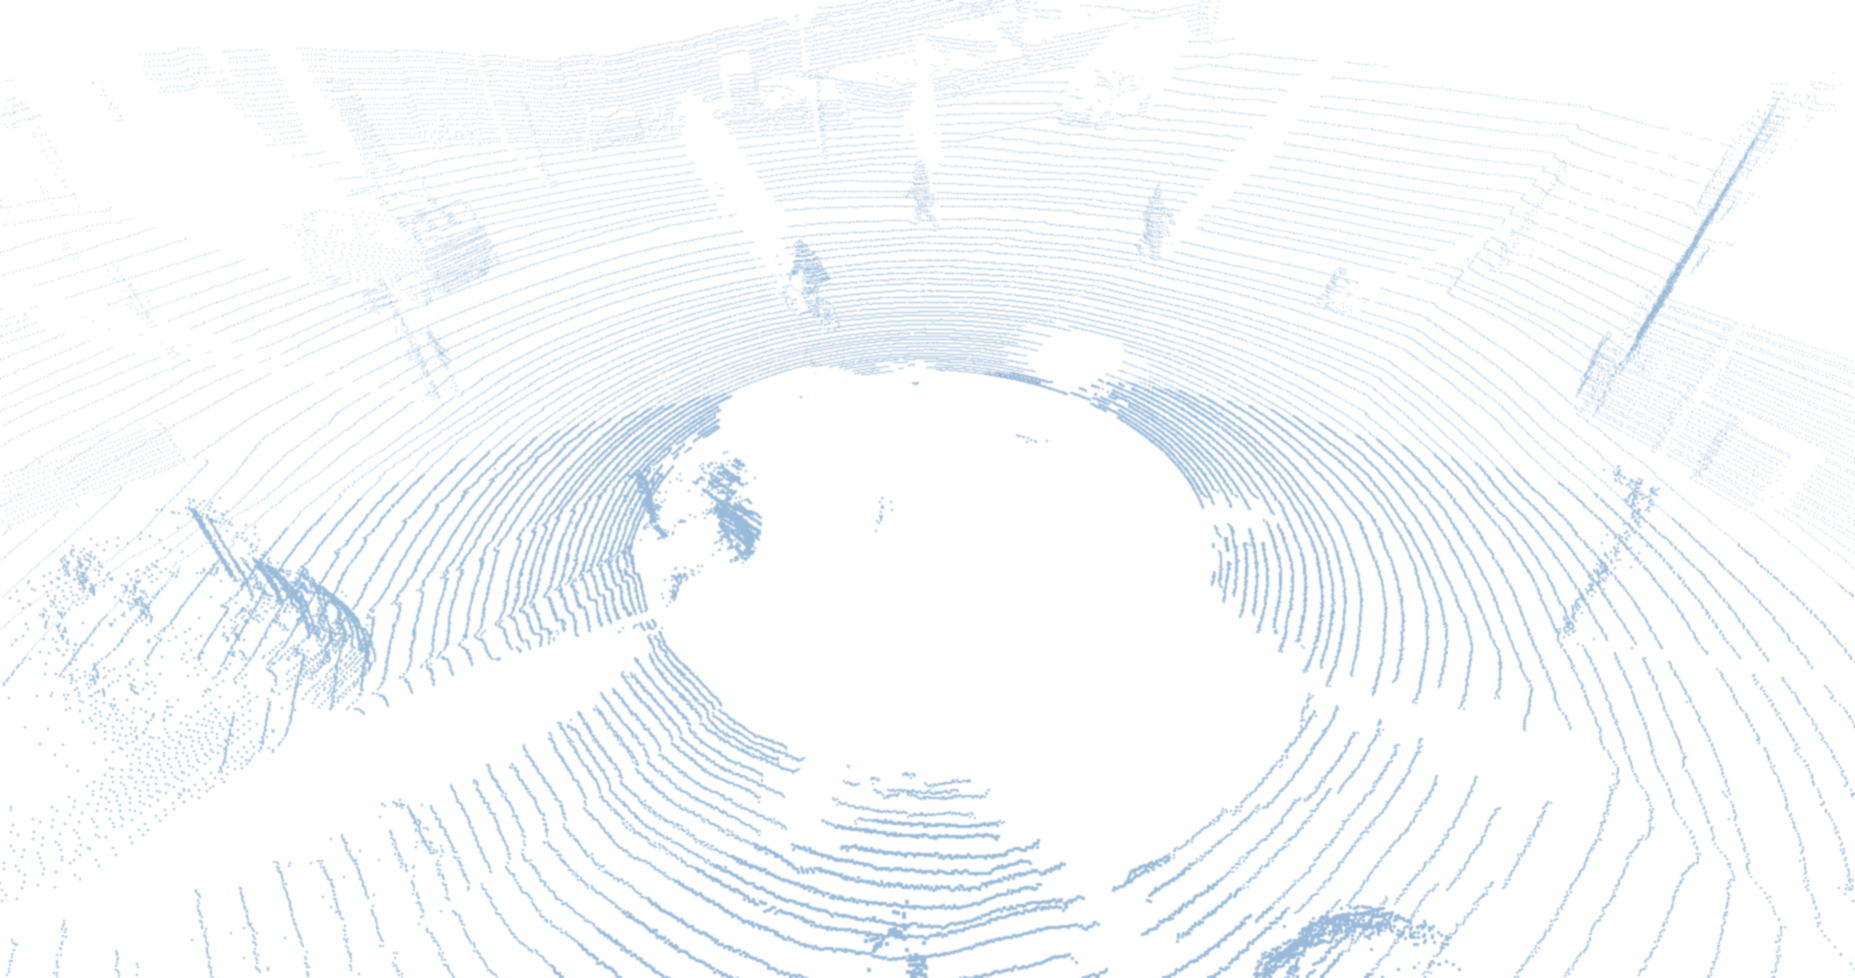
\includegraphics[width=1.425\paperwidth]{images/snapshot01_light}}
  % https://tex.stackexchange.com/questions/30461/beamer-nonumber-equivalent-for-slides
  % https://tex.stackexchange.com/questions/272311/beamers-slide-without-footer
  \begin{frame}[plain,noframenumbering]
    \begin{center}
      \Large{Learning Shape Completion from Bounding Boxes with CAD Shape Priors}\par
      \vskip 6px
      
      \normalsize{David Stutz}\par
      \vskip 6px
      \small{Master Thesis}\par
      \small{September 15th 2017}
    \end{center}
  \end{frame}
  }
  
  % Style the frame footer
  \setbeamertemplate{footline}{
    % Use the predefined command
    \RWTHfooter{\hfill \insertframenumber}
  }
  
  \begin{frame}
    {\large Outline}
    
    \begin{itemize}
      \item Problem
      \item Related Work
      \item Proposed Approach
      \begin{itemize}
        \item Shape Prior
        \item Shape Inference
      \end{itemize}
      \item Experiments
      \item Conclusion
    \end{itemize}
  \end{frame}
  
  \begin{frame}[plain,noframenumbering]
    \begin{center}
      {\Large Problem}
    \end{center}
  \end{frame}
  
  \begin{frame}
    {\large Problem Overview}
    \begin{center}
      Shape completion from point clouds.
    \end{center}
    
    \vspace{-0.5cm}
    \begin{tikzpicture}
      \begin{scope}[on background layer]
        \node at (0,0.5) {
          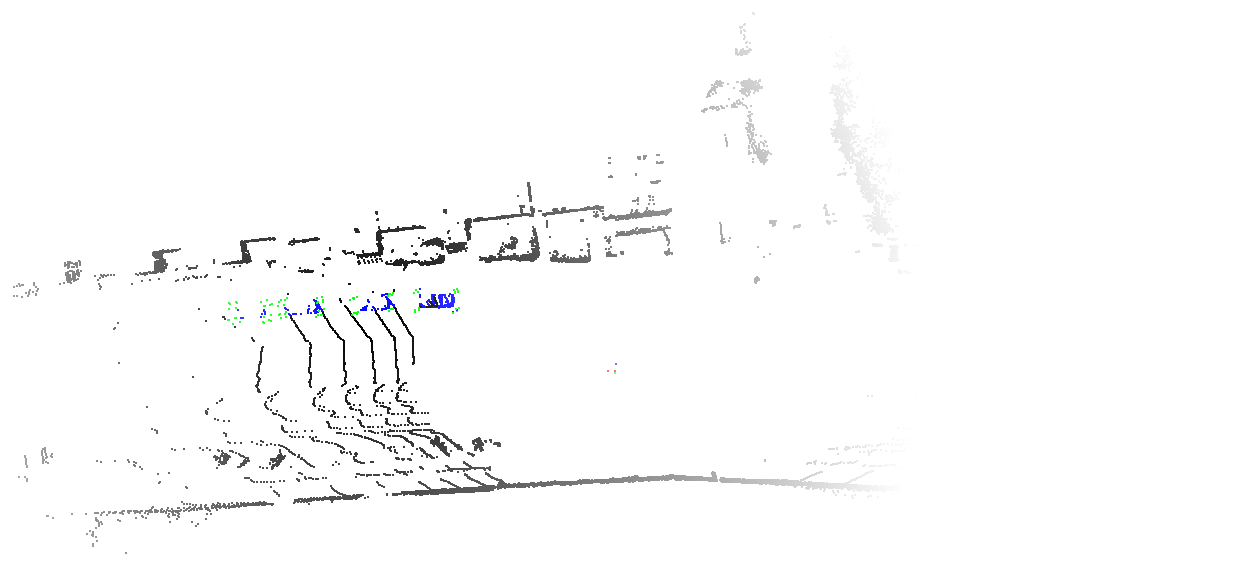
\includegraphics[width=8cm]{images/snapshot00_rect_fade}
        };
      \end{scope}
      
      \node[rectangle,draw=black,fill=white] at (-1.65, -2) {
        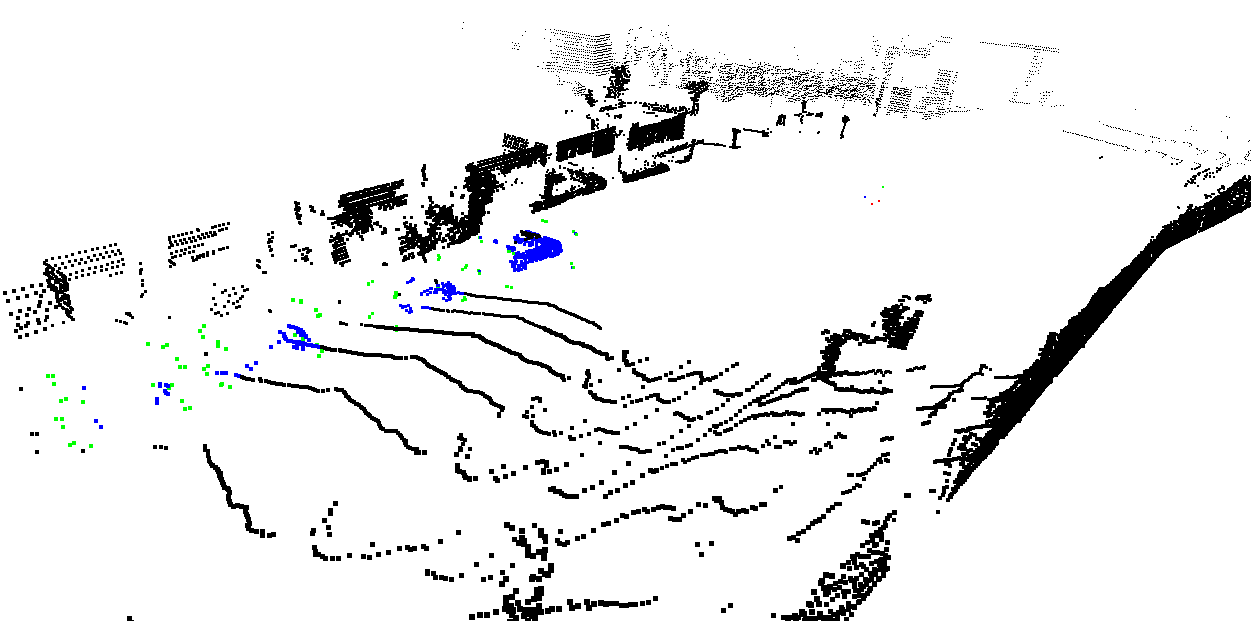
\includegraphics[height=2.25cm]{images/snapshot03_rect}
      };

      \node[rectangle,draw=black,fill=white] at (2.6, -2) {
        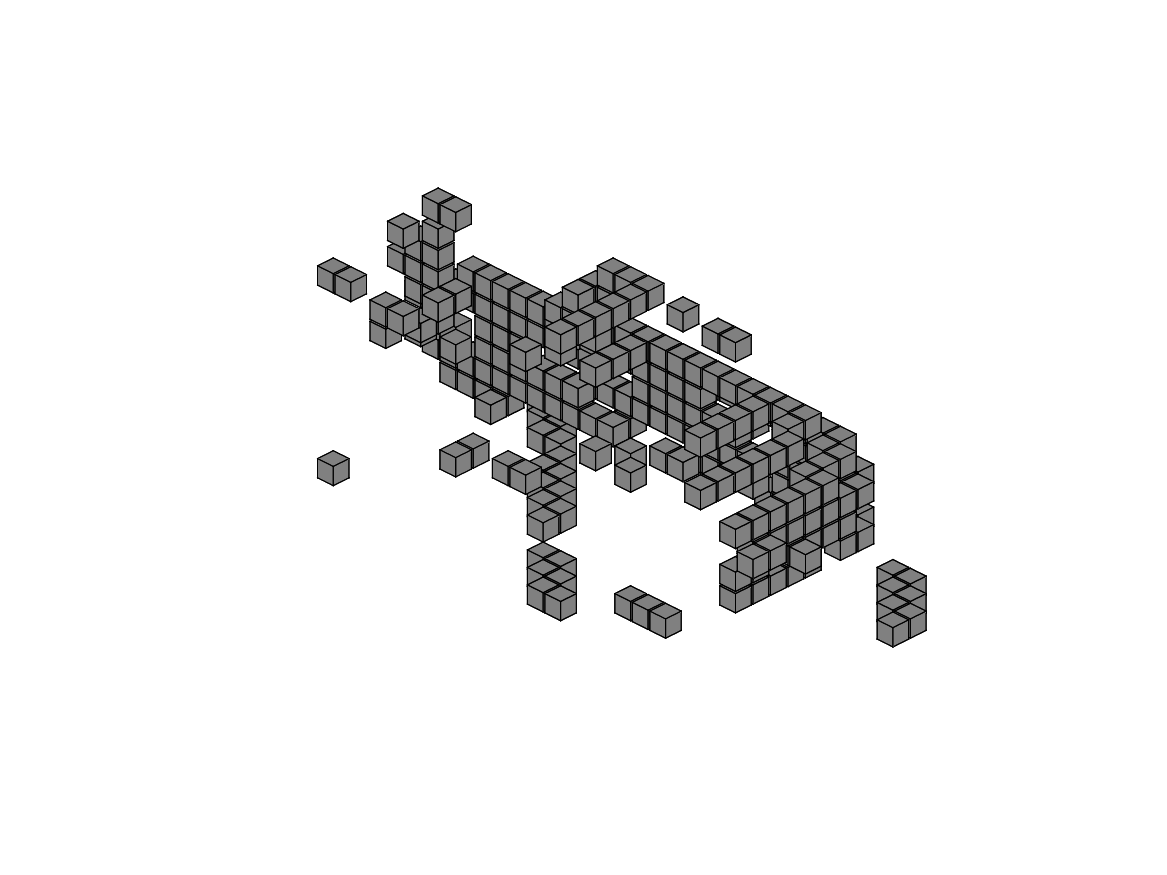
\includegraphics[height=2.25cm,trim={3cm 2cm 3cm 2cm},clip]{images/0_input_45}
      };
      \node at (2.6, -3.65) {\Scriptsize Voxelized Observation};
      
      \node[rectangle,draw=black,fill=white] at (6, -2) {
        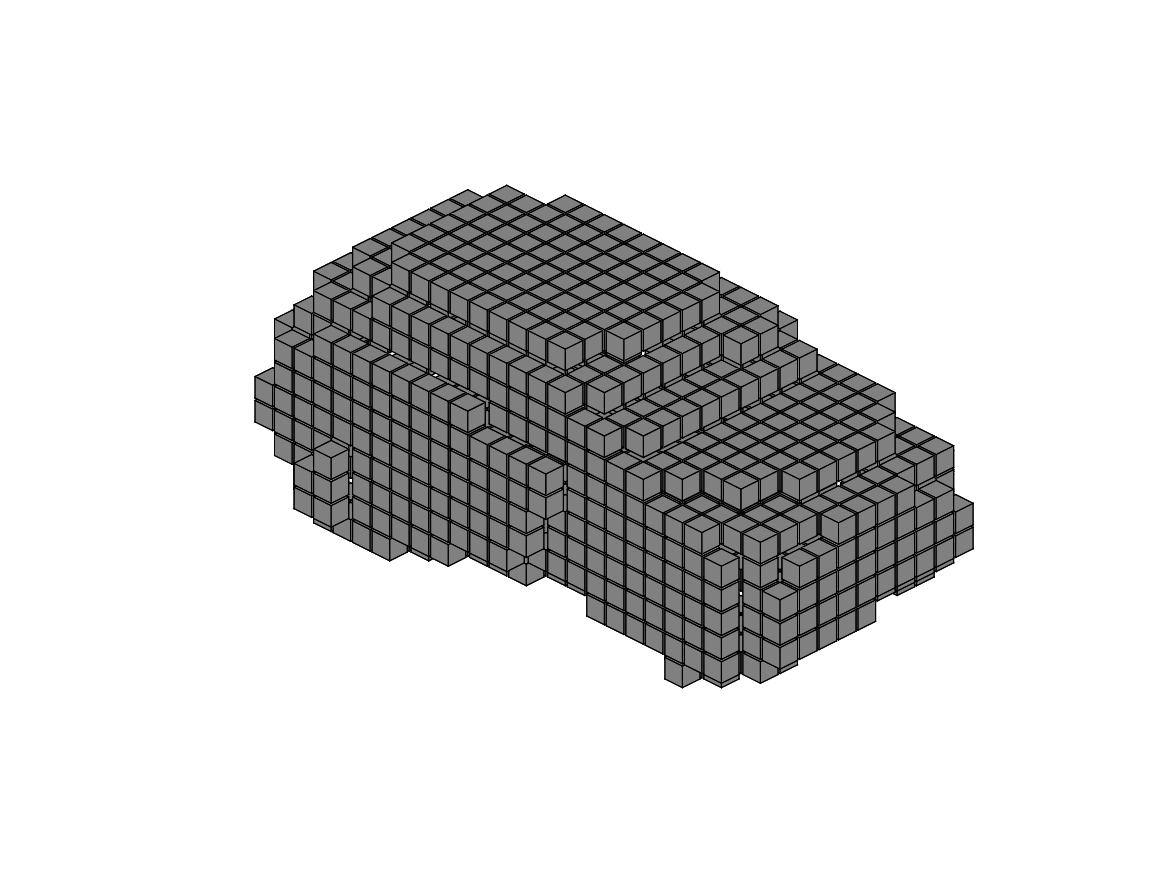
\includegraphics[height=2.25cm,trim={3cm 2cm 3cm 2cm},clip]{images/0_baseline_prediction_45}
      };
      \node at (6, -3.675) {\Scriptsize Voxelized Shape};
    \end{tikzpicture}
    \vspace{1cm}
  \end{frame}
  
  \begin{frame}[t]
    {\large Problem Definition}
    
    \begin{problem}
      \small
      Given
      observations $\mathcal{X} = \{x_1, \ldots, x_N\}$
      and
      reference shapes $\mathcal{Y} = \{y_1, \ldots, y_M\}$,
      learn a mapping $x_n \mapsto y(x_n)$
      such that $y(x_n)$ fits the 
      unknown target shape $y_n^*$.
    \end{problem}
    
    \begin{center}
      %\vspace{0.5cm}
      \begin{tikzpicture}
        \node[transparent,rectangle,draw=black,fill=white] at (-3, 0.7) {
          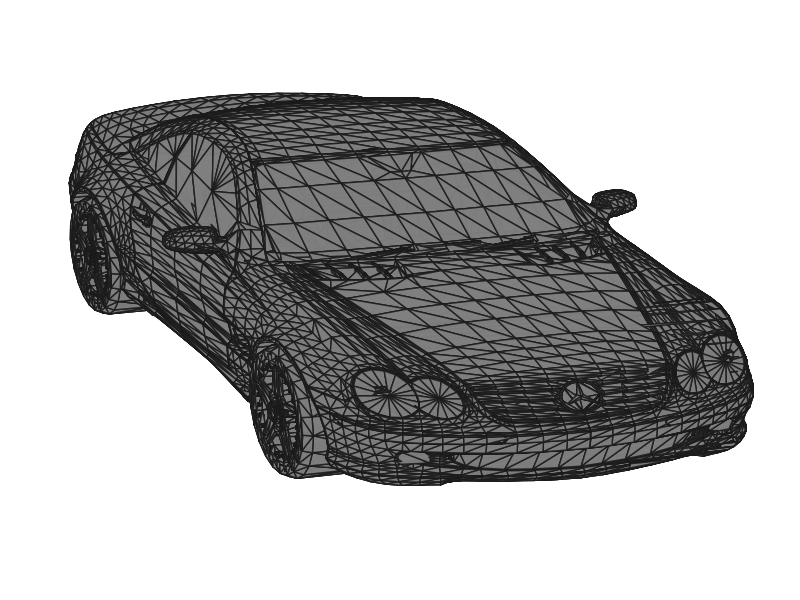
\includegraphics[height=1cm]{images/119033fe083145e22f31600ac759c763}
        };
        \node[transparent,rectangle,draw=black,fill=white] at (-3, -0.7) {
          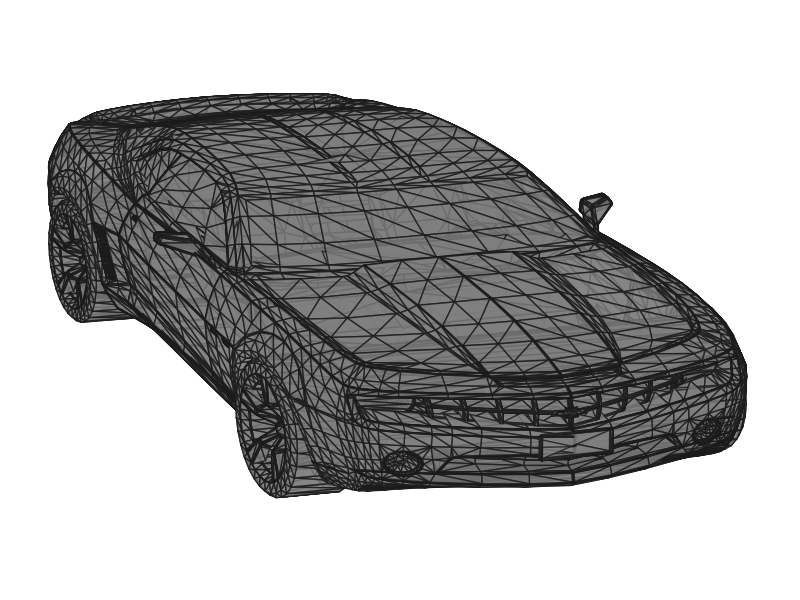
\includegraphics[height=1cm]{images/1137cd58d6a45c6659a47b1880958de9}
        };
        \node[transparent,rectangle,draw=black,fill=white] at (-1.25, 0.7) {
          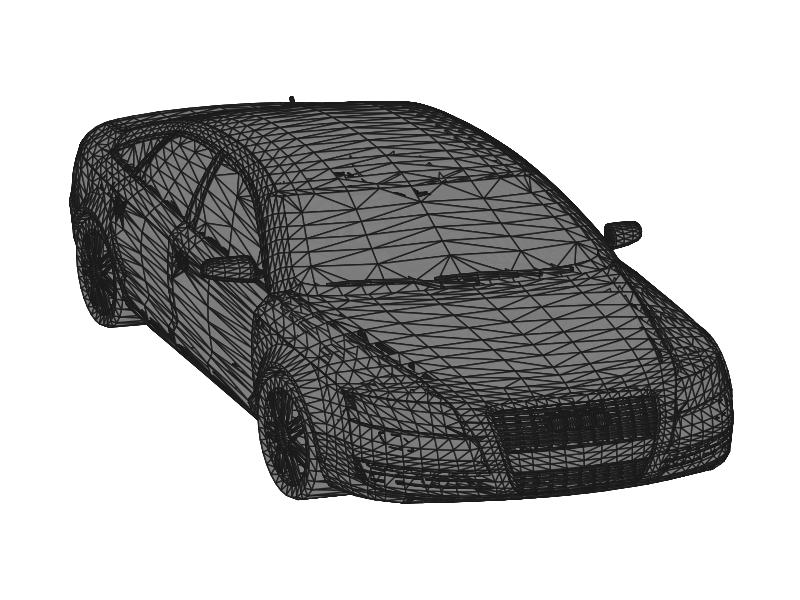
\includegraphics[height=1cm]{images/1104f0924e03f2b6fc5886e868449015}
        };
        \node[transparent,rectangle,draw=black,fill=white] at (-1.25, -0.7) {
          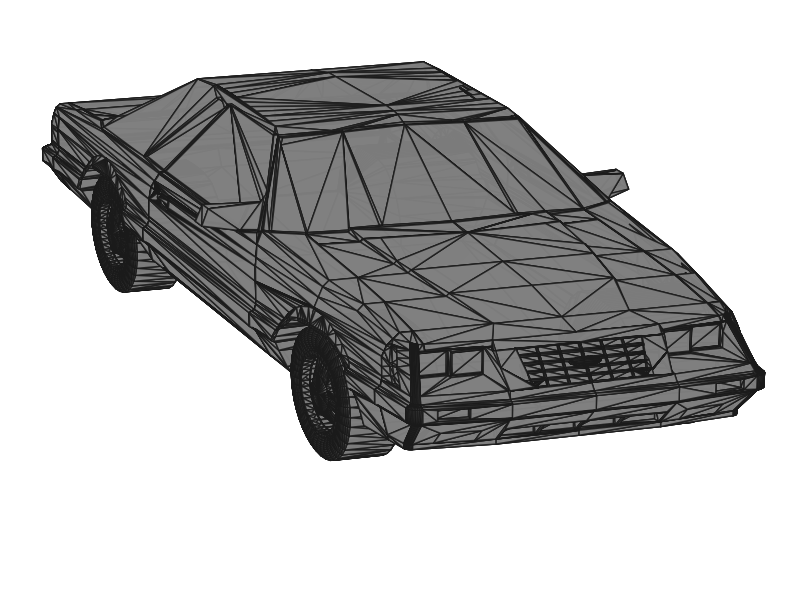
\includegraphics[height=1cm]{images/1089cbe82dc0e72133d7c9e122eec9b6}
        };
        \node[transparent] at (-2.125, -1.75) {\Scriptsize Reference Shapes $y_m$};
        
        \node[rectangle,draw=black,fill=white] at (1.4, 0) {
          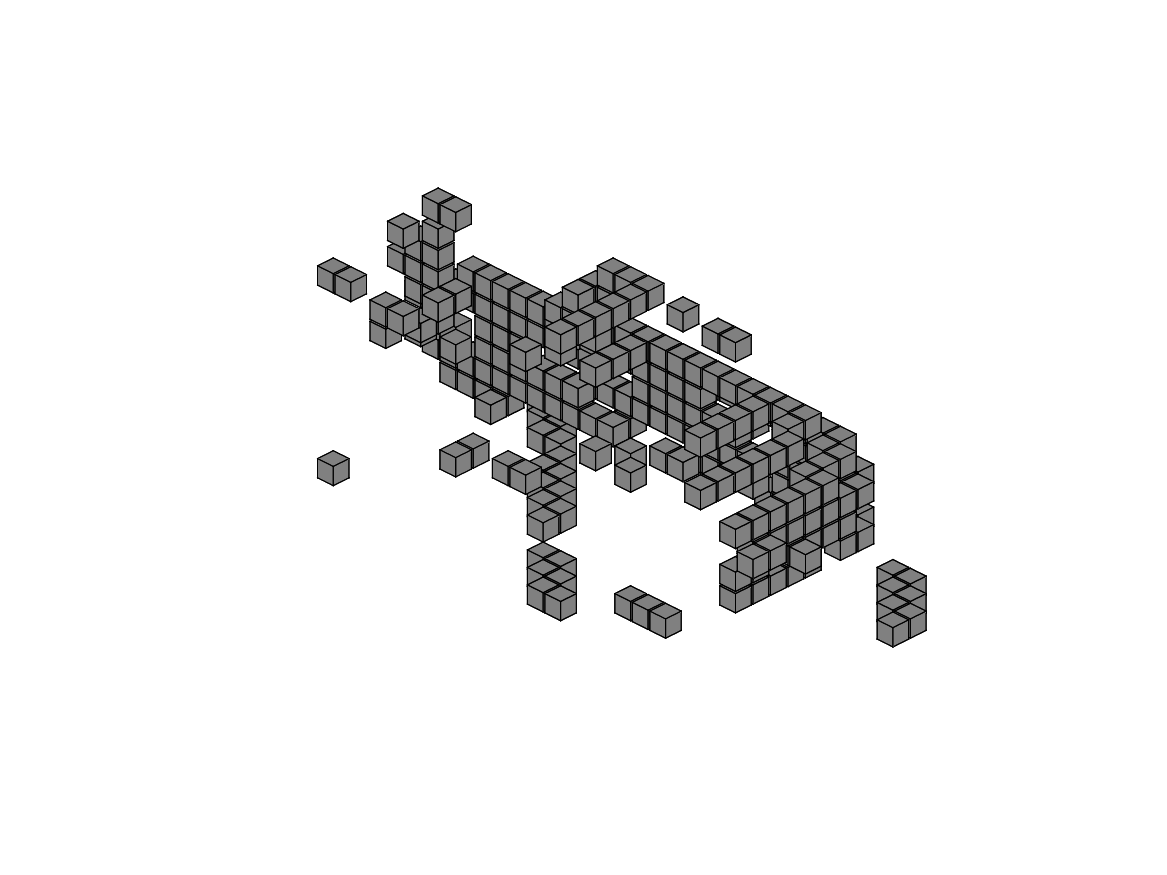
\includegraphics[height=2.4cm,trim={3cm 2cm 3cm 2cm},clip]{images/0_input_45}
        };
        \node at (1.4, -1.75) {\Scriptsize Observation $x_n$};
        
        \node[transparent,rectangle,draw=black,fill=white] at (4.9, 0) {
          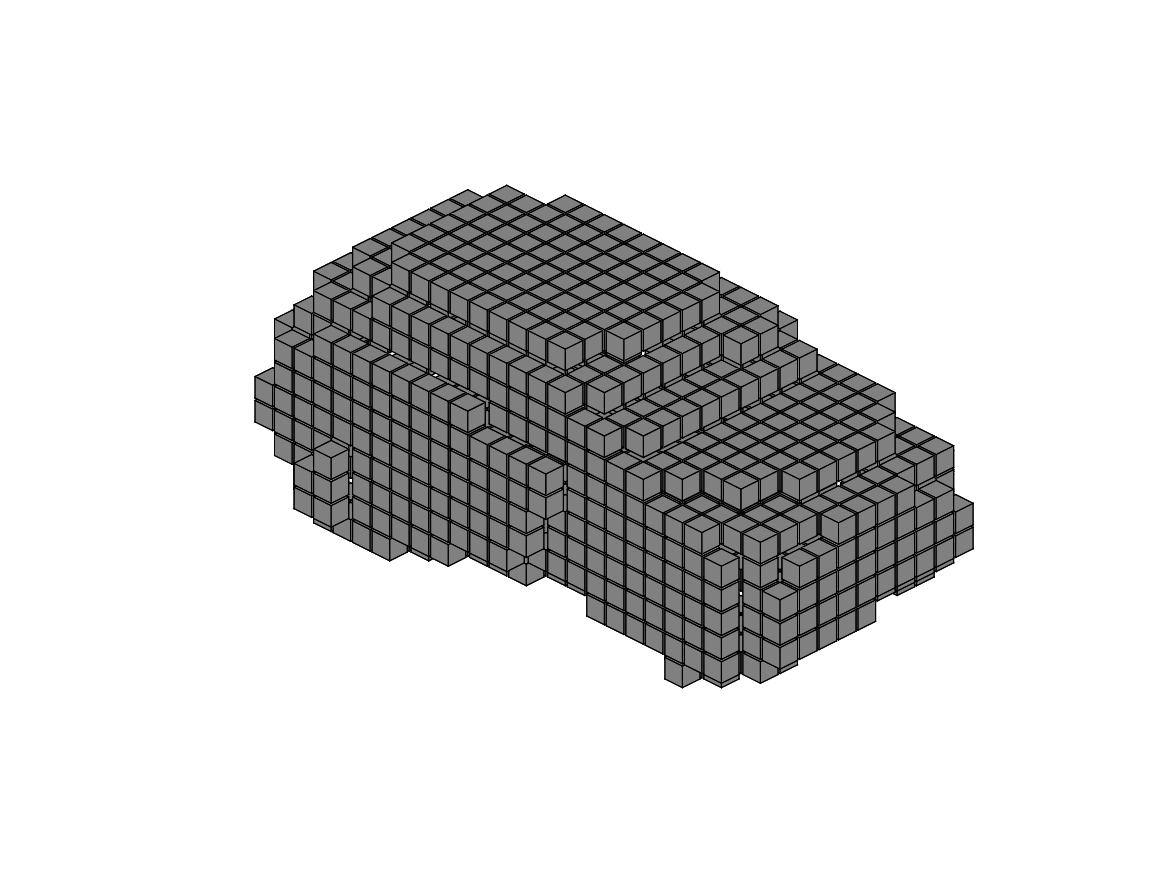
\includegraphics[height=2.4cm,trim={3cm 2cm 3cm 2cm},clip]{images/0_baseline_prediction_45}
        };
        \node[transparent] at (4.9, -1.75) {\Scriptsize Unknown Shape $y_n^*$};
      \end{tikzpicture}
    \end{center}
  \end{frame}
  
  \begin{frame}[t]
    {\large Problem Definition}
    
    \begin{problem}
      \small
      Given
      observations $\mathcal{X} = \{x_1, \ldots, x_N\}$
      and
      reference shapes $\mathcal{Y} = \{y_1, \ldots, y_M\}$,
      learn a mapping $x_n \mapsto y(x_n)$
      such that $y(x_n)$ fits the 
      unknown target shape $y_n^*$.
    \end{problem}
    
    \begin{center}
      %\vspace{0.5cm}
      \begin{tikzpicture}
        \node[rectangle,draw=black,fill=white] at (-3, 0.7) {
          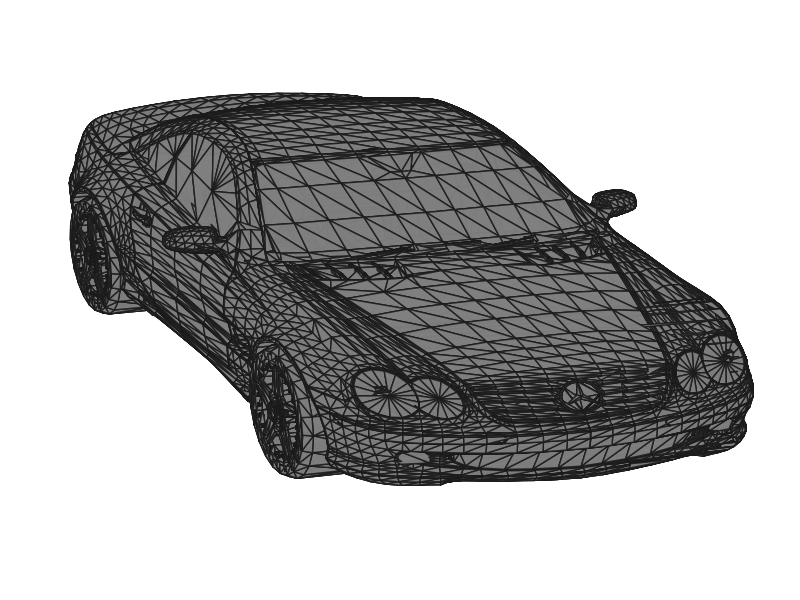
\includegraphics[height=1cm]{images/119033fe083145e22f31600ac759c763}
        };
        \node[rectangle,draw=black,fill=white] at (-3, -0.7) {
          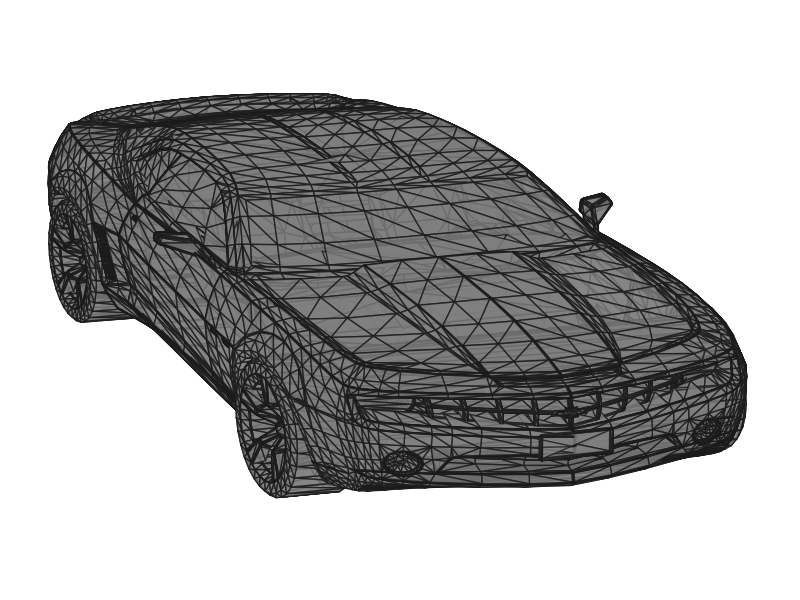
\includegraphics[height=1cm]{images/1137cd58d6a45c6659a47b1880958de9}
        };
        \node[rectangle,draw=black,fill=white] at (-1.25, 0.7) {
          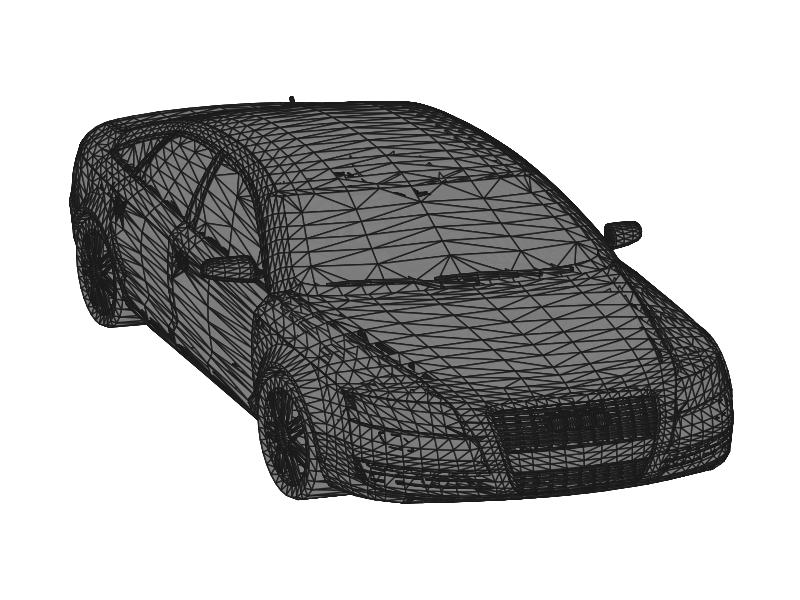
\includegraphics[height=1cm]{images/1104f0924e03f2b6fc5886e868449015}
        };
        \node[rectangle,draw=black,fill=white] at (-1.25, -0.7) {
          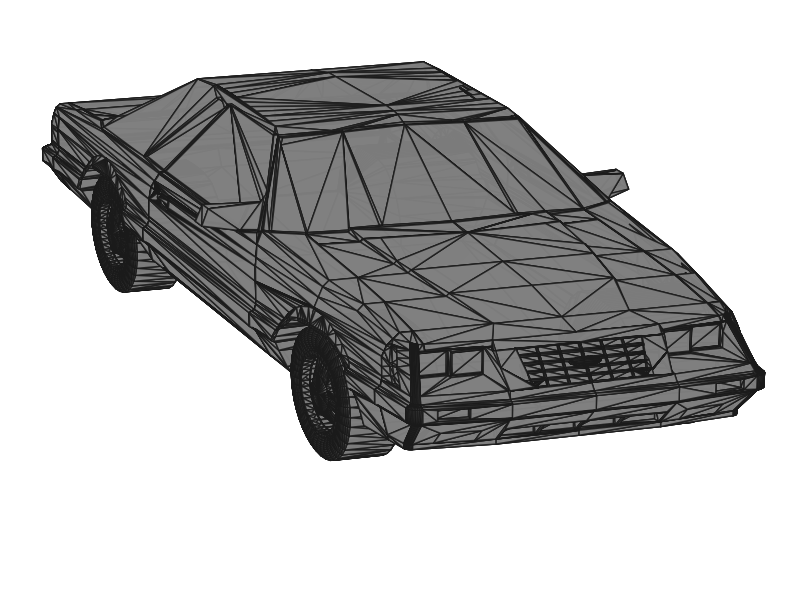
\includegraphics[height=1cm]{images/1089cbe82dc0e72133d7c9e122eec9b6}
        };
        \node at (-2.125, -1.75) {\Scriptsize Reference Shapes $y_m$};
        
        \node[rectangle,draw=black,fill=white] at (1.4, 0) {
          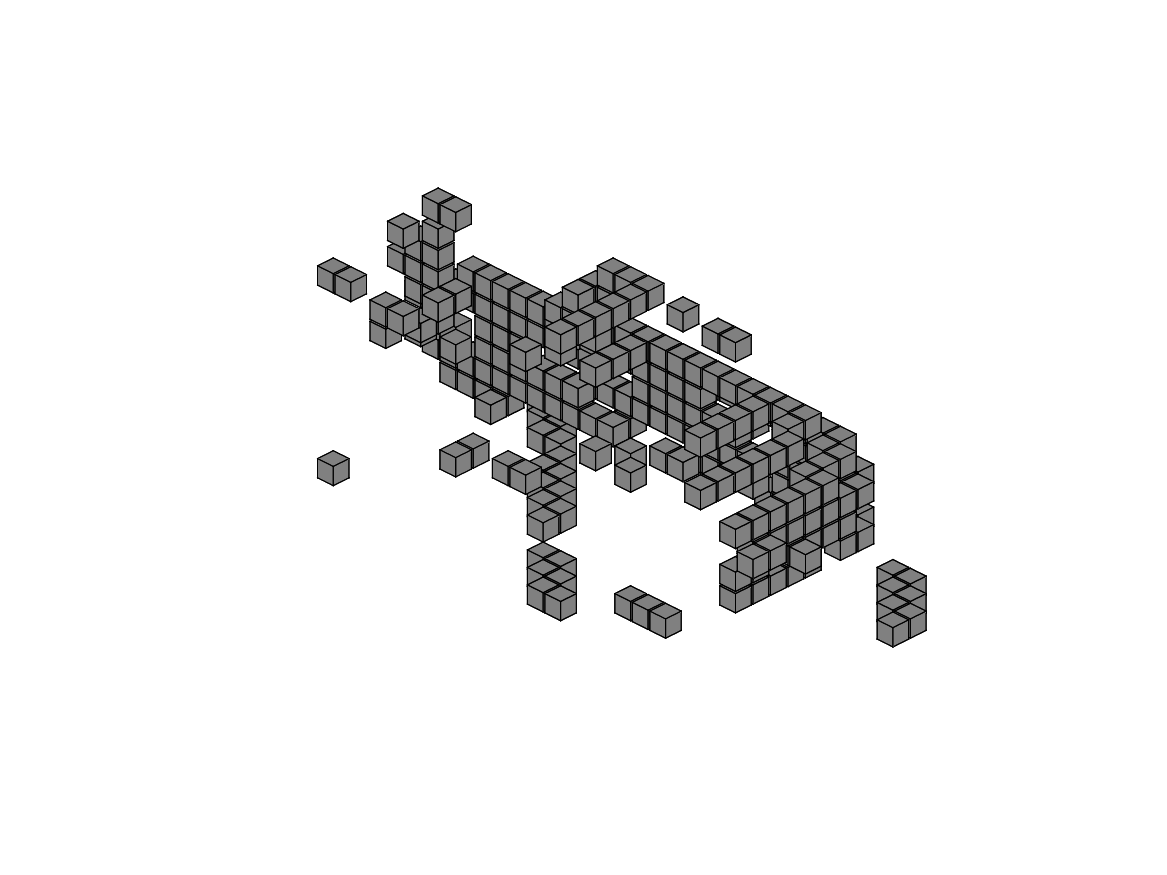
\includegraphics[height=2.4cm,trim={3cm 2cm 3cm 2cm},clip]{images/0_input_45}
        };
        \node at (1.4, -1.75) {\Scriptsize Observation $x_n$};
        
        \node[transparent,rectangle,draw=black,fill=white] at (4.9, 0) {
          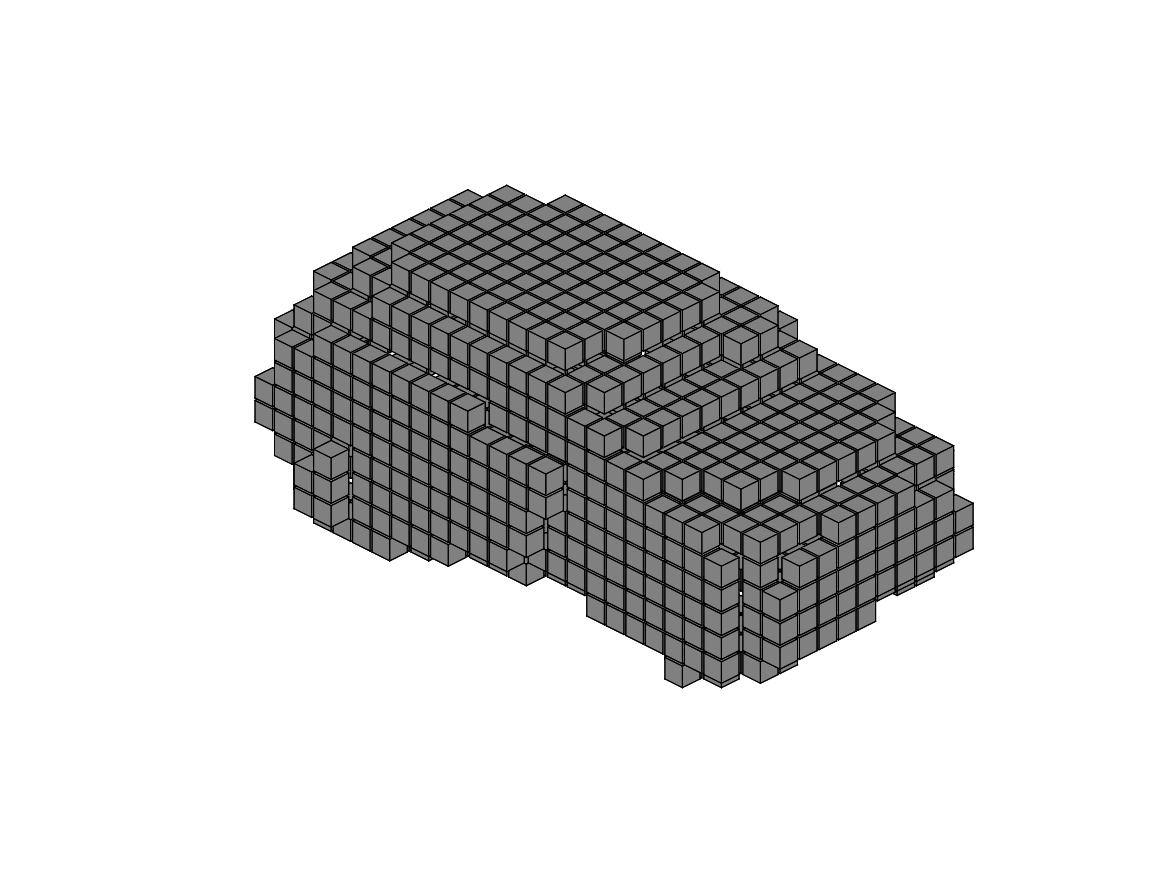
\includegraphics[height=2.4cm,trim={3cm 2cm 3cm 2cm},clip]{images/0_baseline_prediction_45}
        };
        \node[transparent] at (4.9, -1.75) {\Scriptsize Unknown Shape $y_n^*$};
      \end{tikzpicture}
    \end{center}
  \end{frame}
  
  \begin{frame}[t]
    {\large Problem Definition}
    
    \begin{problem}
      \small
      Given
      observations $\mathcal{X} = \{x_1, \ldots, x_N\}$
      and
      reference shapes $\mathcal{Y} = \{y_1, \ldots, y_M\}$,
      learn a mapping $x_n \mapsto y(x_n)$
      such that $y(x_n)$ fits the 
      {\color{RWTHred}unknown target shape $y_n^*$}.
    \end{problem}
    
    \begin{center}
      %\vspace{0.5cm}
      \begin{tikzpicture}
        \node[rectangle,draw=black,fill=white] at (-3, 0.7) {
          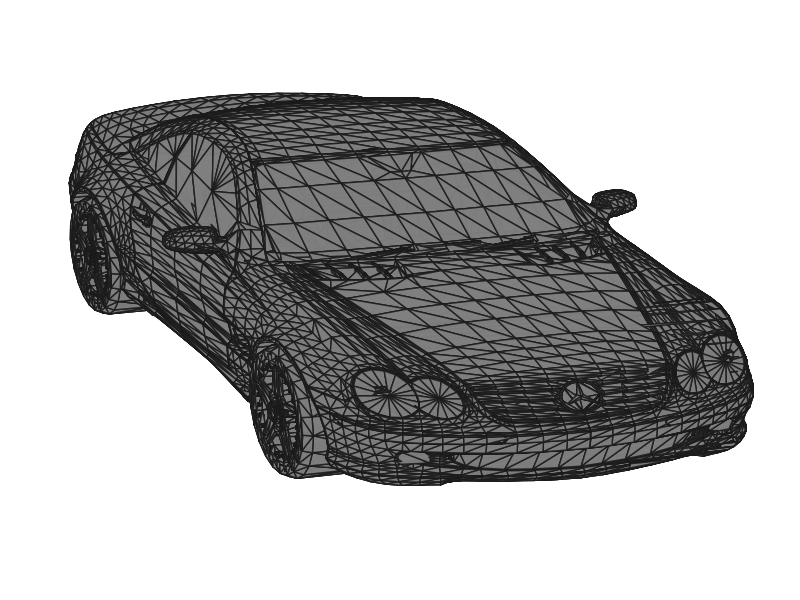
\includegraphics[height=1cm]{images/119033fe083145e22f31600ac759c763}
        };
        \node[rectangle,draw=black,fill=white] at (-3, -0.7) {
          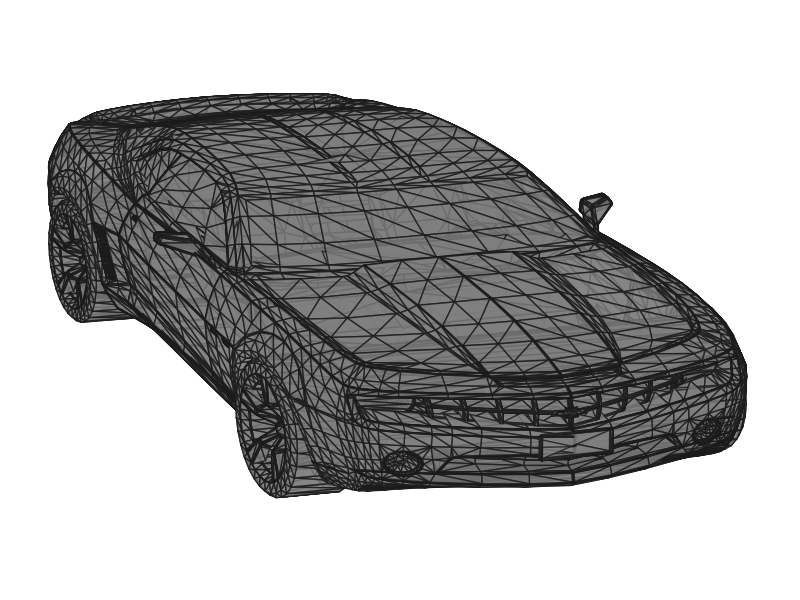
\includegraphics[height=1cm]{images/1137cd58d6a45c6659a47b1880958de9}
        };
        \node[rectangle,draw=black,fill=white] at (-1.25, 0.7) {
          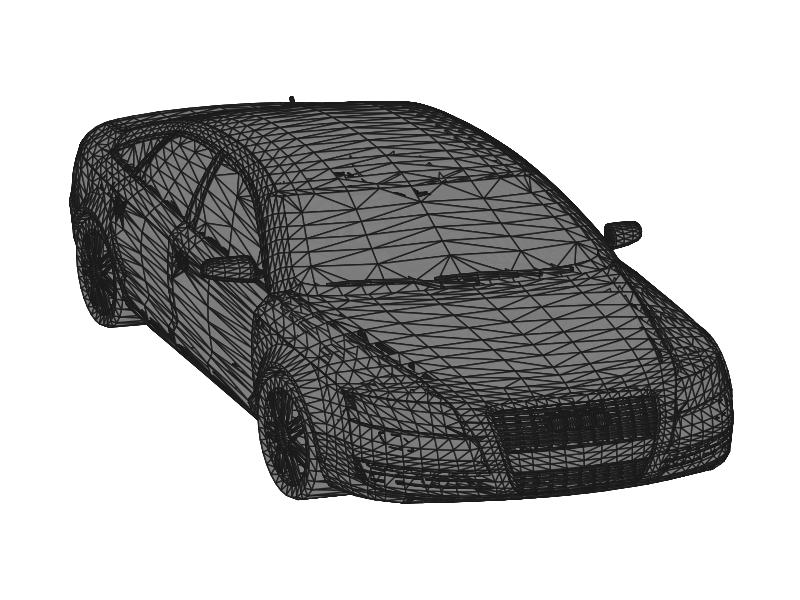
\includegraphics[height=1cm]{images/1104f0924e03f2b6fc5886e868449015}
        };
        \node[rectangle,draw=black,fill=white] at (-1.25, -0.7) {
          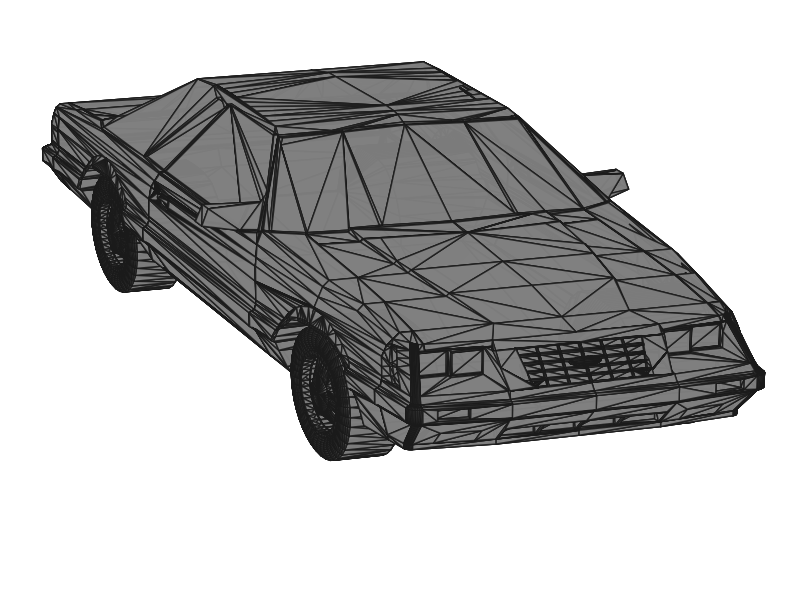
\includegraphics[height=1cm]{images/1089cbe82dc0e72133d7c9e122eec9b6}
        };
        \node at (-2.125, -1.75) {\Scriptsize Reference Shapes $y_m$};
        
        \node[rectangle,draw=black,fill=white] at (1.4, 0) {
          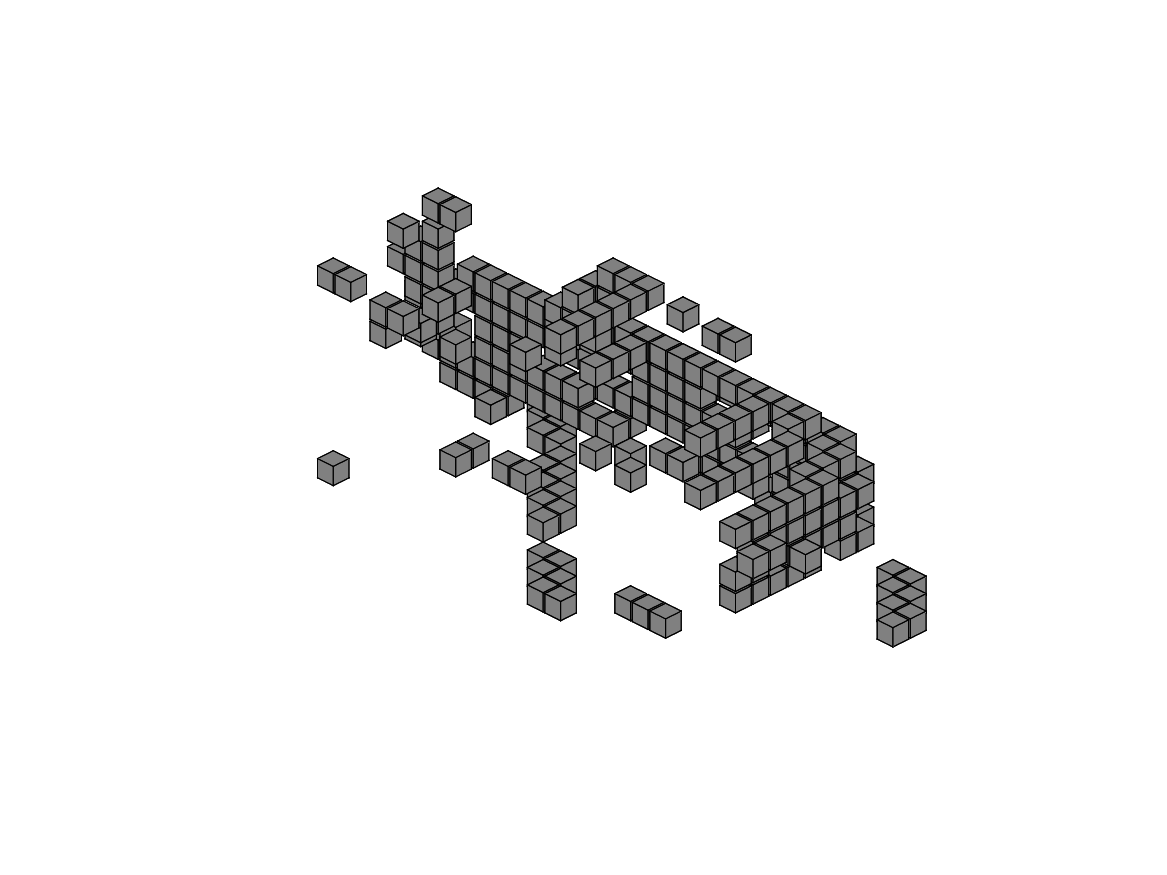
\includegraphics[height=2.4cm,trim={3cm 2cm 3cm 2cm},clip]{images/0_input_45}
        };
        \node at (1.4, -1.75) {\Scriptsize Observation $x_n$};
        
        \node[rectangle,draw=RWTHred,fill=white] at (4.9, 0) {
          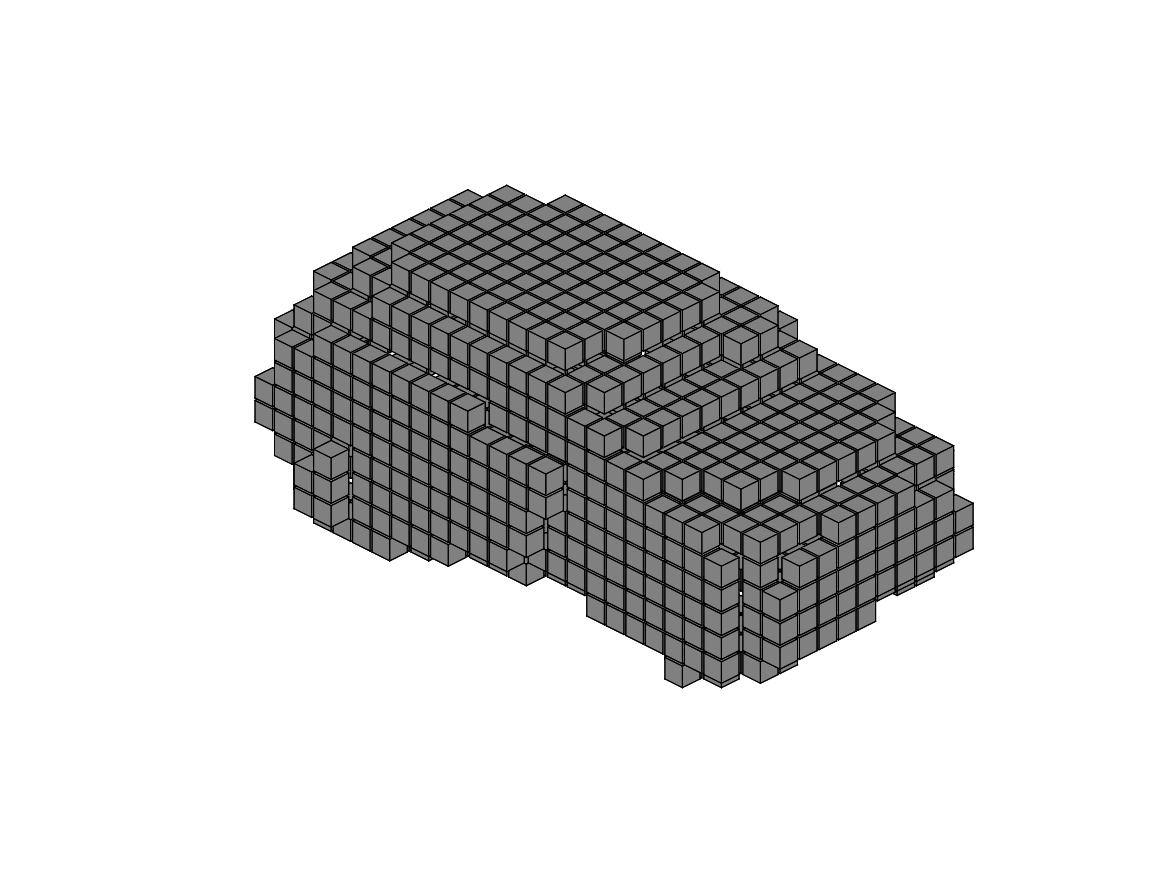
\includegraphics[height=2.4cm,trim={3cm 2cm 3cm 2cm},clip]{images/0_baseline_prediction_45}
        };
        \node at (4.9, -1.75) {\Scriptsize\color{RWTHred} Unknown Shape $y_n^*$};
      \end{tikzpicture}
    \end{center}
  \end{frame}
  
  \begin{frame}[t]
    {\large Problem Definition}
    
    \begin{problem}
      \small
      Given
      observations $\mathcal{X} = \{x_1, \ldots, x_N\}$
      and
      reference shapes $\mathcal{Y} = \{y_1, \ldots, y_M\}$,
      learn a mapping $x_n \mapsto y(x_n)$
      such that $y(x_n)$ fits the 
      {\color{RWTHred}unknown target shape $y_n^*$}.
    \end{problem}
    %\vspace{-0.5cm}
    
    Weakly-supervised: 
    \begin{itemize}
      \item known object category;
      \item and bounding boxes required on real data.
    \end{itemize}
  \end{frame}
  
  \begin{frame}[plain,noframenumbering]
    \begin{center}
      {\Large Related Work}
    \end{center}
  \end{frame}
  
  \begin{frame}
    {\large Related Work}
    
    Generative shape modeling, including \cite{WuSongXiao:2015,WuTenenbaum:2016}.
    \pause
    \vspace{1em}
    
    Shape completion, following \cite{SungAngstGuibas:2015}:
    \begin{itemize}
      \item symmetry based approaches;
      \item data-driven approaches, including 
      \cite{DameReid:2013,EngelmannStuecklerLeibe:2016};
      \item and recently learning-based approaches, including
      \cite{DaiNiessner:2016}.
    \end{itemize}
  \end{frame}
  
  \begin{frame}
    {\large Selected Related Work}
    
    Generative shape modeling, \eg
    \cite{WuSongXiao:2015,WuTenenbaum:2016}:
    
    \begin{itemize}
      \item Learn a generative model of shapes, \eg using generative adversarial networks \cite{WuTenenbaum:2016};
      \item and use for shape classification, manipulation and generation.
    \end{itemize}
    
    \begin{tikzpicture}
      \node at (2.25, -1.25) {\color{RWTHlightgrey}\tiny \cite{WuTenenbaum:2016}};
      \begin{scope}[on background layer]
        \node[scope fading=south] at (0, 0) {
          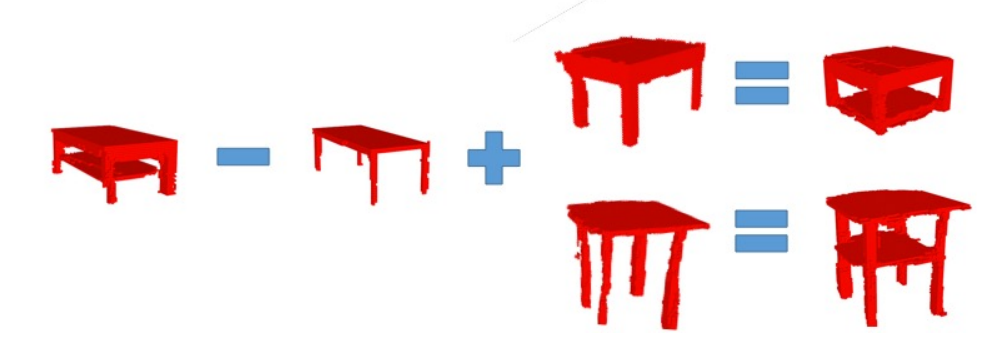
\includegraphics[width=6cm]{images/Wu_2016}
        };
      \end{scope}
      
      \node at (4.25, -1.25) {\color{RWTHlightgrey}\tiny \cite{WuSongXiao:2015}};
      \begin{scope}[on background layer]
        \node[scope fading=south] at (6, 0) {
          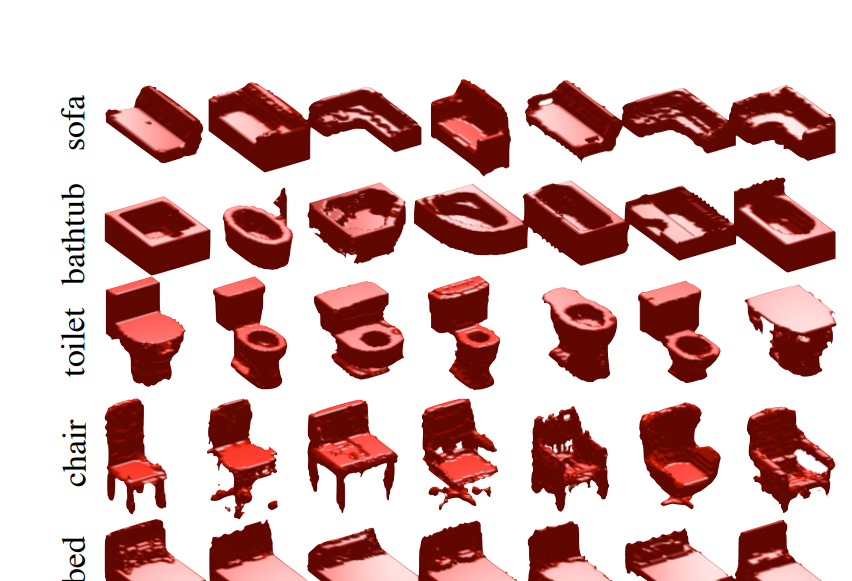
\includegraphics[width=6cm,trim={0 5cm 0 0},clip]{images/Wu_2015}
        };
      \end{scope}
    \end{tikzpicture}
  \end{frame}
  
  \begin{frame}
    {\large Selected Related Work}
    
    Data-driven shape completion, \eg
    \cite{DameReid:2013,EngelmannStuecklerLeibe:2016}:
    \begin{itemize}
      \item Learn shape prior, \eg using PCA or GP-LVM;
      \item and pose shape completion as energy minimization.
    \end{itemize}
    
    \hspace*{4cm}
    \begin{tikzpicture}
      \node at (1.65, -0.5) {\color{RWTHlightgrey}\tiny\cite{EngelmannStuecklerLeibe:2016}};
      \begin{scope}[on background layer]
        \node[] at (-0.5, 1) {
          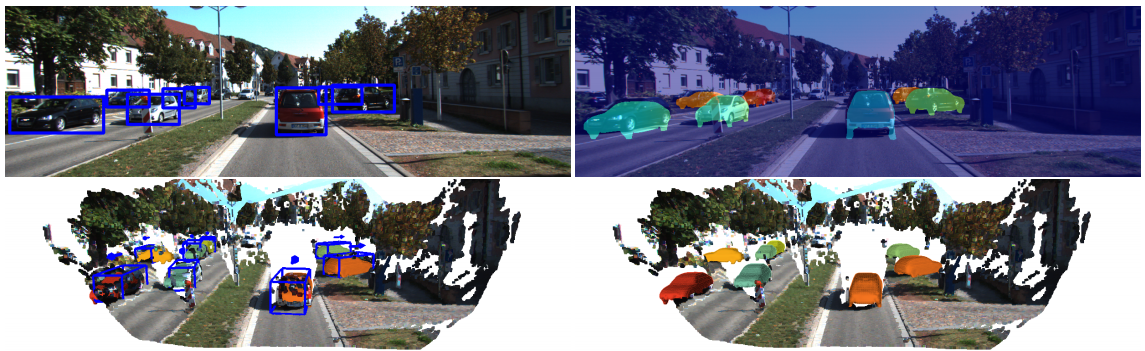
\includegraphics[width=7cm]{images/Engelmann_2016_2}
        };
      \end{scope}
    \end{tikzpicture}
  \end{frame}
  
  \begin{frame}
    {\large Selected Related Work}
    
    Learning-based shape completion, \eg
    \cite{DaiNiessner:2016}:
    \begin{itemize}
      \item Learn an encoder-decoder network on synthetic data;
      \item and post-process if necessary.
    \end{itemize}
    
    \hspace*{0.5cm}
    \begin{tikzpicture}
      \node at (2, -0.25) {\color{RWTHlightgrey}\tiny\cite{DaiNiessner:2016}};
      \begin{scope}[on background layer]
        \node[] at (-0.5, 1) {
          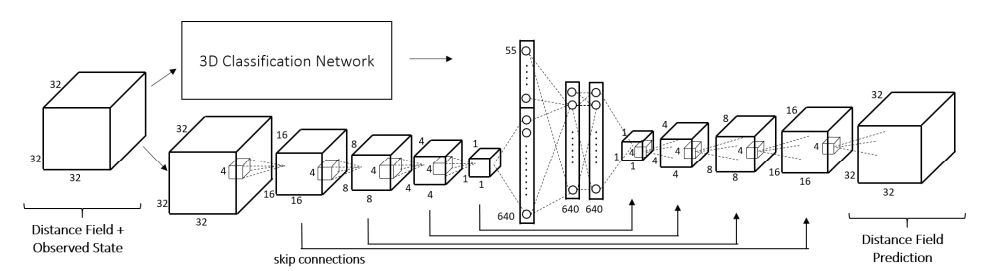
\includegraphics[width=7cm]{images/Dai_2016}
        };
      \end{scope}
      
      \begin{scope}[on background layer]
        \node[scope fading=south] at (5, 0) {
          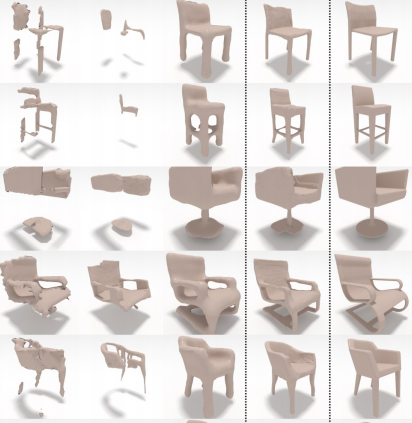
\includegraphics[width=4cm,trim={0 2cm 0 0},clip]{images/Dai_2016_2}
        };
      \end{scope}
    \end{tikzpicture}
  \end{frame}
  
  \begin{frame}
    {\large Discussion}
    
    Two ``philosophies'':
    \begin{itemize}
      \item data-driven approaches are applicable to real data, but shape completion
      involves energy minimization;
      \item learning-based approaches need supervision, but shape completion
      is ``just a forward pass''.
    \end{itemize}
  \end{frame}
  
  \begin{frame}
    {\large Discussion}
    
    \begin{question}
      Do strong shape priors allow us to learn shape completion under weak supervision?
    \end{question}
    
    Goal:
    \begin{itemize}
      \item Efficient shape completion;
      \item and learning on real data.
    \end{itemize}
  \end{frame}
  
  \begin{frame}[plain,noframenumbering]
    \begin{center}
      {\Large Proposed Approach}
    \end{center}
  \end{frame}
  
  \begin{frame}
    {\large Proposed Approach}
    
    \textbf{Shape prior.}\\[6px]
    Learn a variational auto-encoder \cite{KingmaWelling:2013}:
    
    \vspace{-0.25cm}
    \begin{tikzpicture}
      \node (y) at (-1.5, 0) {\footnotesize $y$};
          
      \node[rectangle,draw=black] (input) at (0, 0) {
        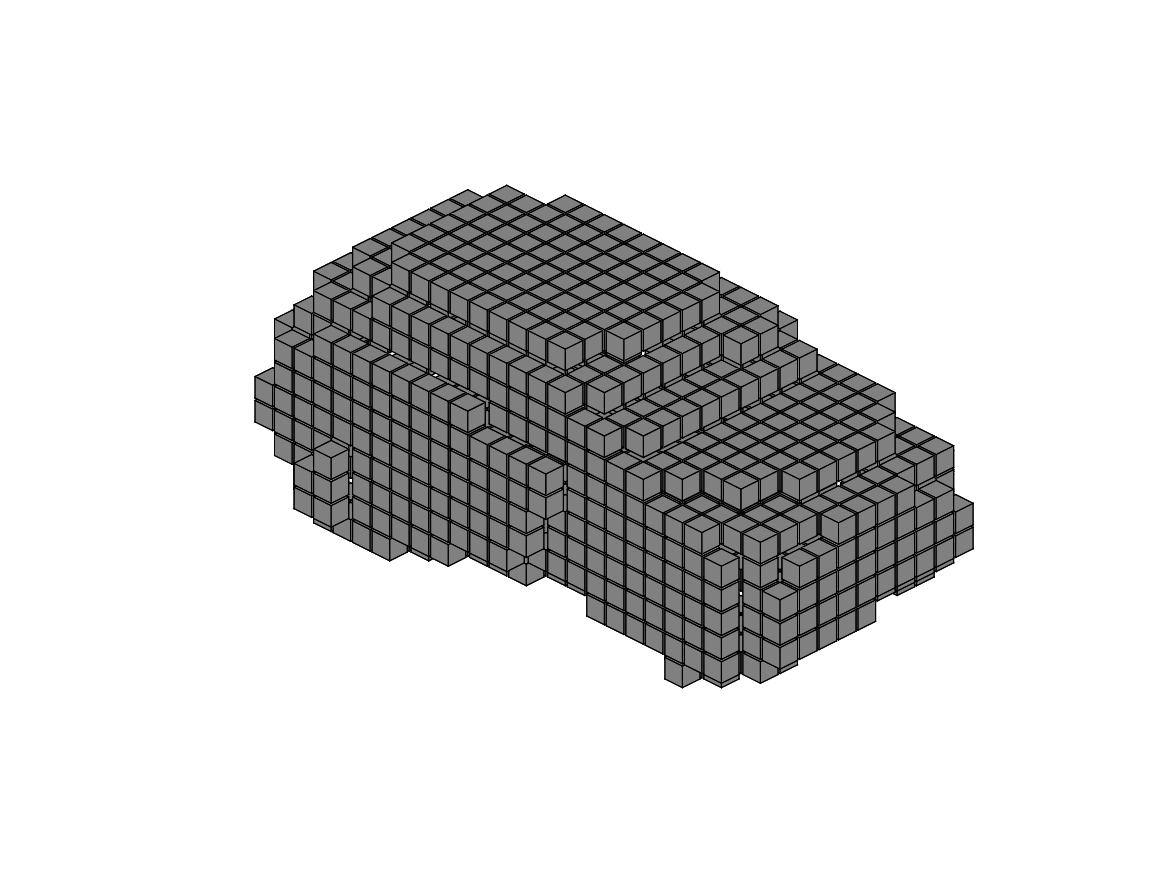
\includegraphics[height=1.5cm,trim={3cm 2cm 3cm 2cm},clip]{images/0_baseline_prediction_45}
      };
      
      \node at (2.3, 0) {\footnotesize Encoder};
      \draw[-] ($(input.north east) + (0.25,0)$) -- (3.25,0.5);
      \draw[-] ($(input.south east) + (0.25,0)$) -- (3.25,-0.5);
      \draw[-] ($(input.south east) + (0.25,0)$) -- ($(input.north east) + (0.25,0)$);
      \draw[-] (3.25,-0.5) -- (3.25,0.5);
      
      \node (z) at (3.5, 0) {\footnotesize $z$};
      
      \node[rectangle,draw=black] (output) at (7, 0) {
        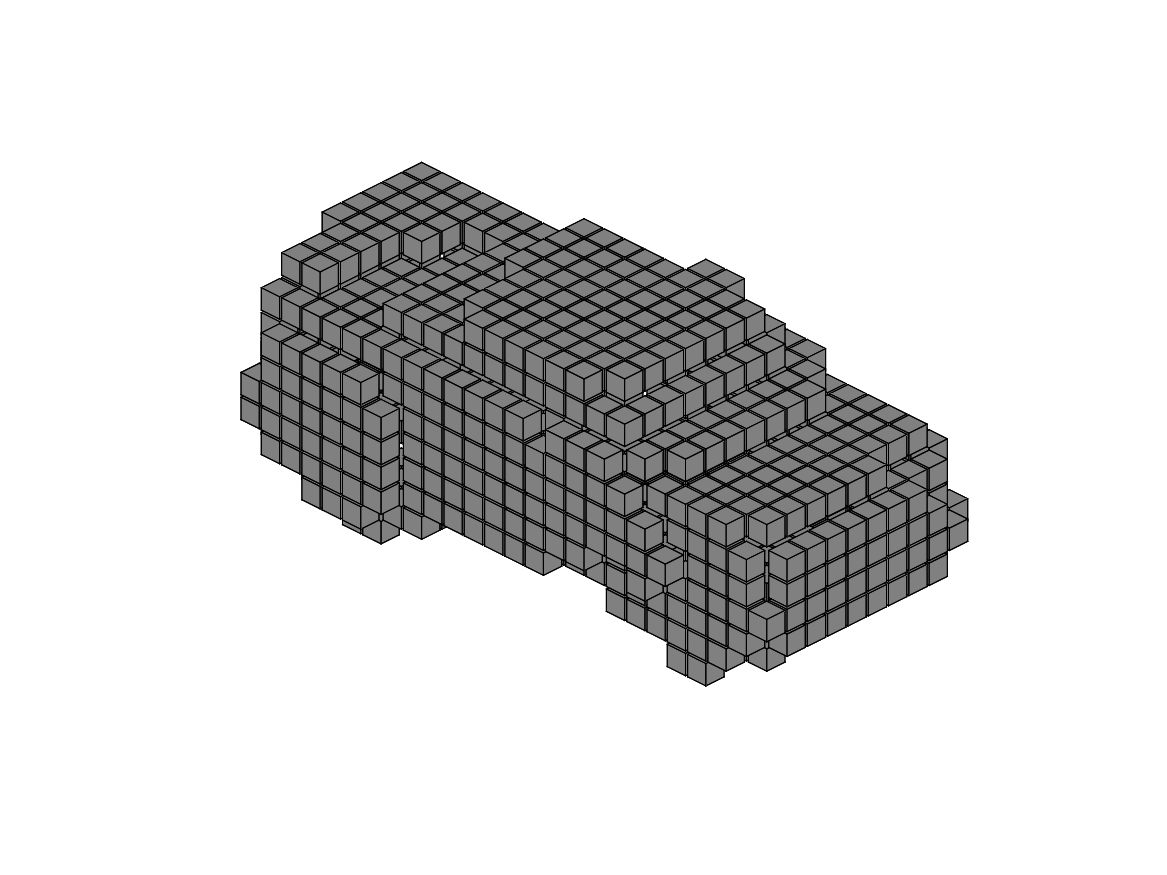
\includegraphics[height=1.5cm,trim={3cm 2cm 3cm 2cm},clip]{images/0_prediction_45}
      };
      
      \node at (4.7, 0) {\footnotesize Decoder};
      \draw[-] ($(output.north west) - (0.25,0)$) -- (3.75,0.5);
      \draw[-] ($(output.south west) - (0.25,0)$) -- (3.75,-0.5);
      \draw[-] ($(output.south west) - (0.25,0)$) -- ($(output.north west) - (0.25,0)$);
      \draw[-] (3.75,-0.5) -- (3.75,0.5);
      
      \node (ry) at (8.5, 0) {\footnotesize $\tilde{y}$};
      
      \node[transparent,color=RWTHdarkorange] at (0.5,1.4) {\footnotesize Recognition Model $q(z|y)$};
      \node[transparent,rectangle,dashed,draw=RWTHdarkorange,minimum width=5.2cm,minimum height=3cm] at (0.7, 0.25) {};
      
      \node[transparent,color=RWTHgreen] at (6,1.4) {\footnotesize Generative Model $p(y|z) p(z)$};
      \node[transparent,rectangle,dashed,draw=RWTHgreen,minimum width=5.5cm,minimum height=3cm] at (6.1, 0.25) {};
      
      \node[transparent] (L) at (3.5, -2) {\footnotesize Reconstruction and Prior Loss};
        
      \draw[transparent,-] (ry) -- ($(ry) - (0,2)$);
      \draw[transparent,-] ($(ry) - (0,2)$) -- (L);
      \draw[transparent,-] (y) -- ($(y) - (0,2)$);
      \draw[transparent,-] ($(y) - (0,2)$) -- (L);
    \end{tikzpicture}
  \end{frame}
  
  \begin{frame}
    {\large Proposed Approach}
    
    \textbf{Shape prior.}\\[6px]
    Learn a variational auto-encoder:
    
    \vspace{0.5cm}
    \begin{tikzpicture}
      \node (y) at (-1.5, 0) {\footnotesize $y$};
          
      \node[rectangle,draw=black] (input) at (0, 0) {
        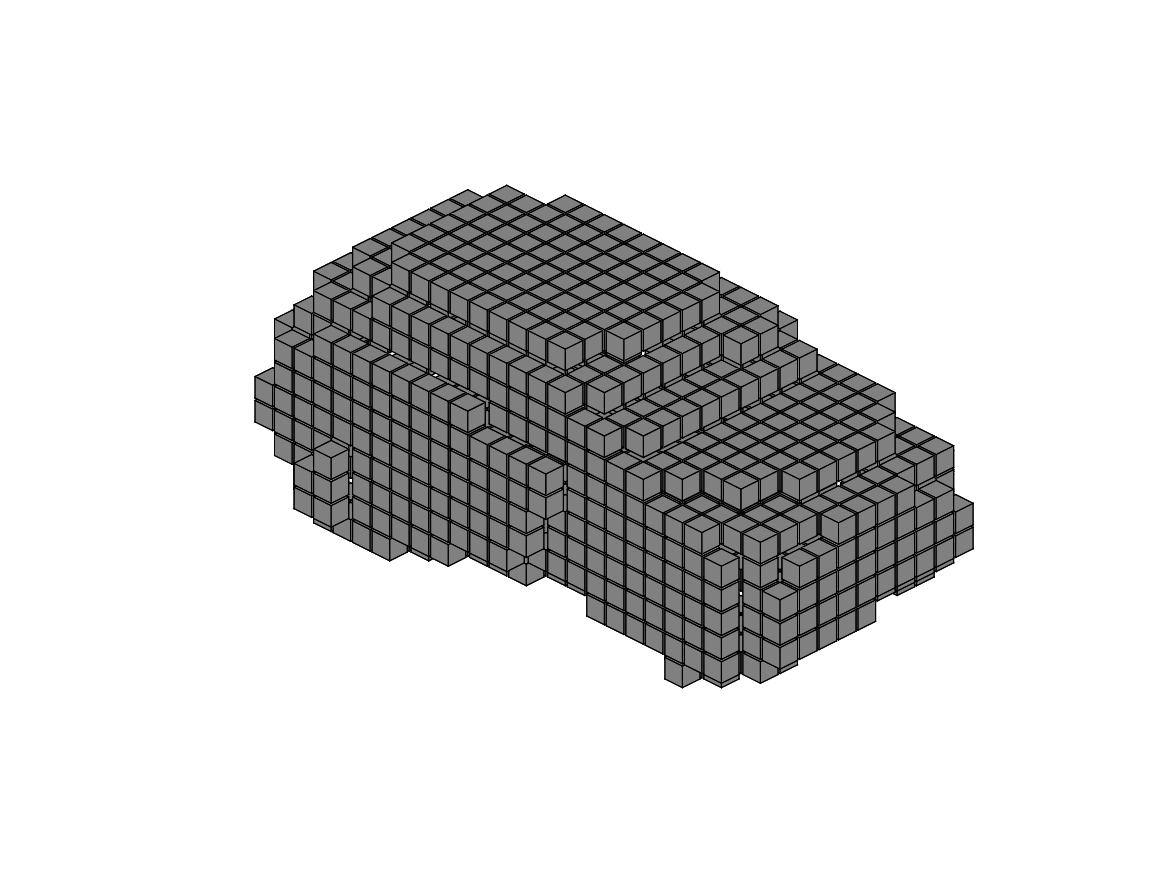
\includegraphics[height=1.5cm,trim={3cm 2cm 3cm 2cm},clip]{images/0_baseline_prediction_45}
      };
      
      \node at (2.3, 0) {\footnotesize Encoder};
      \draw[-] ($(input.north east) + (0.25,0)$) -- (3.25,0.5);
      \draw[-] ($(input.south east) + (0.25,0)$) -- (3.25,-0.5);
      \draw[-] ($(input.south east) + (0.25,0)$) -- ($(input.north east) + (0.25,0)$);
      \draw[-] (3.25,-0.5) -- (3.25,0.5);
      
      \node (z) at (3.5, 0) {\footnotesize $z$};
      
      \node[rectangle,draw=black] (output) at (7, 0) {
        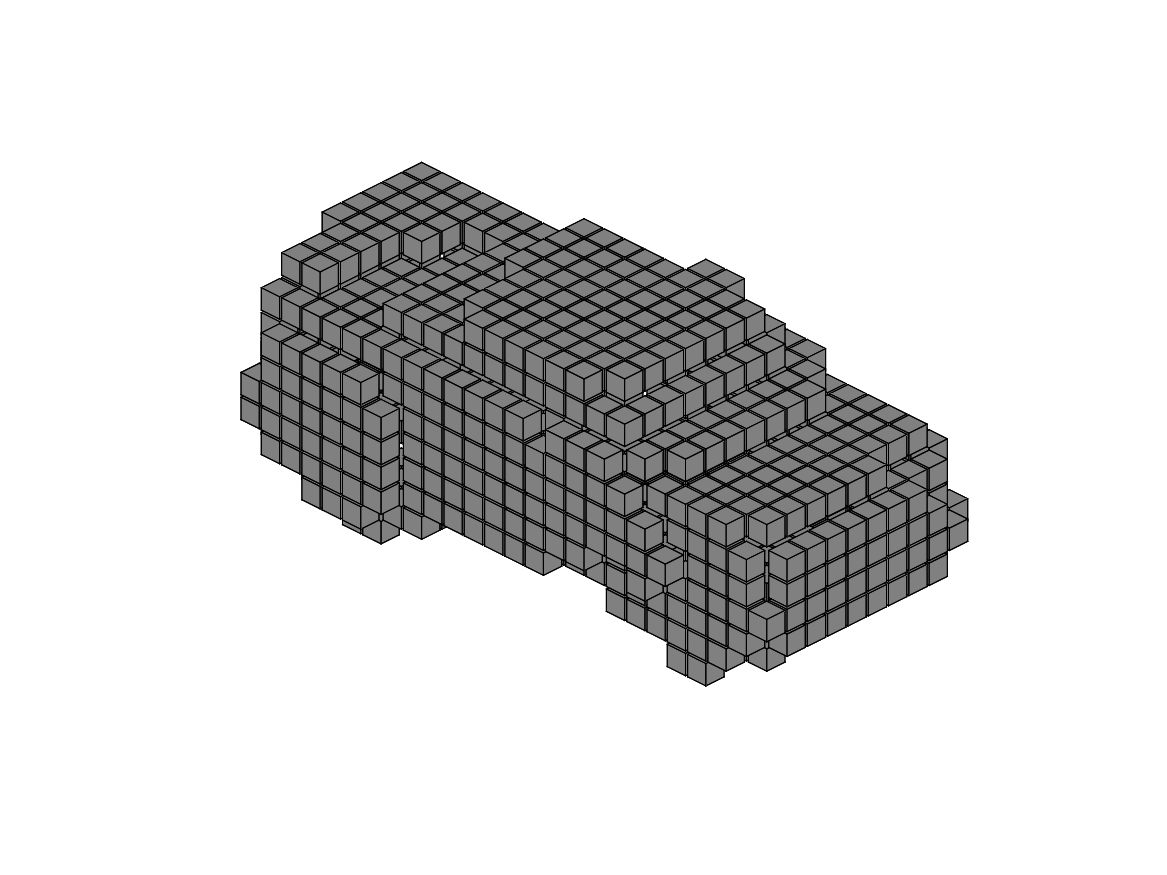
\includegraphics[height=1.5cm,trim={3cm 2cm 3cm 2cm},clip]{images/0_prediction_45}
      };
      
      \node at (4.7, 0) {\footnotesize Decoder};
      \draw[-] ($(output.north west) - (0.25,0)$) -- (3.75,0.5);
      \draw[-] ($(output.south west) - (0.25,0)$) -- (3.75,-0.5);
      \draw[-] ($(output.south west) - (0.25,0)$) -- ($(output.north west) - (0.25,0)$);
      \draw[-] (3.75,-0.5) -- (3.75,0.5);
      
      \node (ry) at (8.5, 0) {\footnotesize $\tilde{y}$};
      
      \node[transparent,color=RWTHdarkorange] at (0.5,1.4) {\footnotesize Recognition Model $q(z|y)$};
      \node[transparent,rectangle,dashed,draw=RWTHdarkorange,minimum width=5.2cm,minimum height=3cm] at (0.7, 0.25) {};
      
      \node[transparent,color=RWTHgreen] at (6,1.4) {\footnotesize Generative Model $p(y|z) p(z)$};
      \node[transparent,rectangle,dashed,draw=RWTHgreen,minimum width=5.5cm,minimum height=3cm] at (6.1, 0.25) {};
      
      \node[] (L) at (3.5, -2) {\footnotesize Reconstruction and Prior Loss};
      
      \draw[-] (ry) -- ($(ry) - (0,2)$);
      \draw[-] ($(ry) - (0,2)$) -- (L);
      \draw[-] (y) -- ($(y) - (0,2)$);
      \draw[-] ($(y) - (0,2)$) -- (L);
    \end{tikzpicture}
  \end{frame}
  
  \begin{frame}
    {\large Proposed Approach}
    
    \textbf{Shape prior.}\\[6px]
    Learn a variational auto-encoder:
    
    \vspace{0.5cm}
    \begin{tikzpicture}
      \node (y) at (-1.5, 0) {\footnotesize $y$};
          
      \node[rectangle,draw=black] (input) at (0, 0) {
        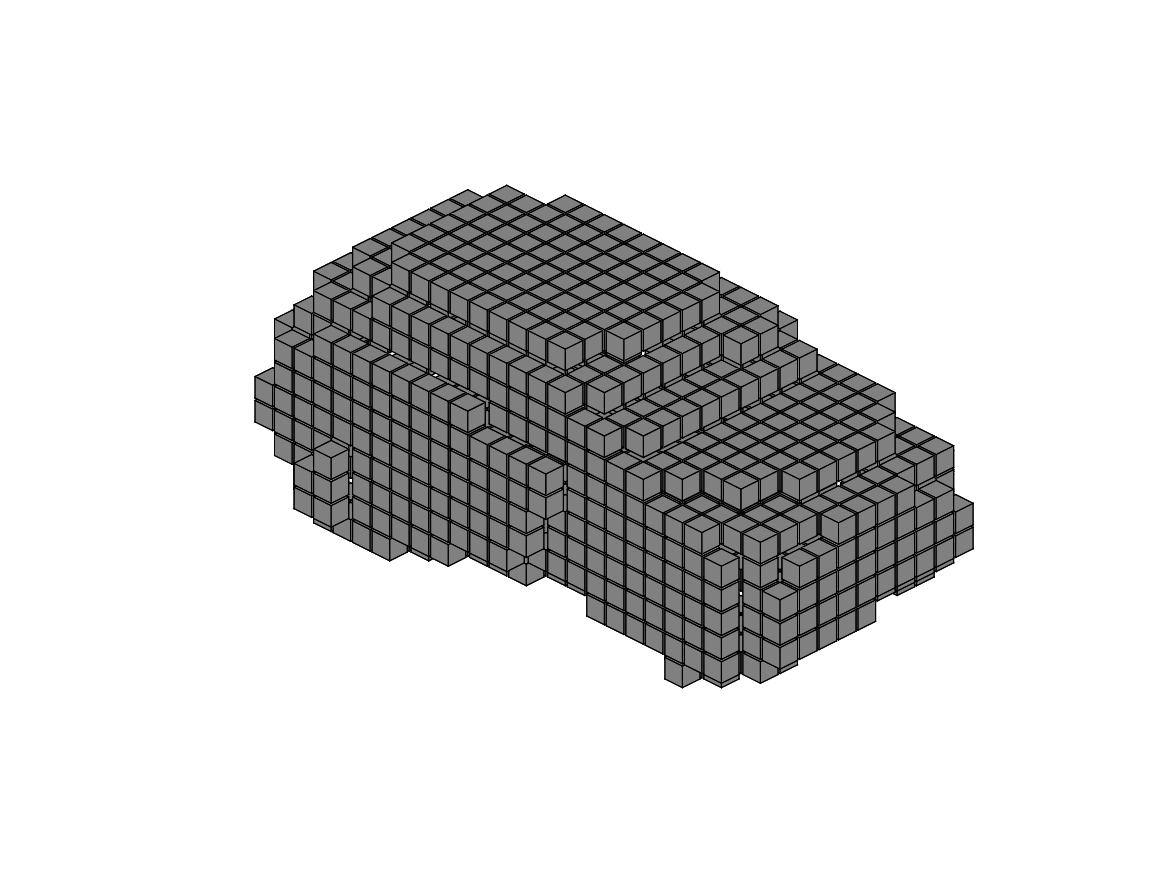
\includegraphics[height=1.5cm,trim={3cm 2cm 3cm 2cm},clip]{images/0_baseline_prediction_45}
      };
      
      \node at (2.3, 0) {\footnotesize Encoder};
      \draw[-] ($(input.north east) + (0.25,0)$) -- (3.25,0.5);
      \draw[-] ($(input.south east) + (0.25,0)$) -- (3.25,-0.5);
      \draw[-] ($(input.south east) + (0.25,0)$) -- ($(input.north east) + (0.25,0)$);
      \draw[-] (3.25,-0.5) -- (3.25,0.5);
      
      \node (z) at (3.5, 0) {\footnotesize $z$};
      
      \node[rectangle,draw=black] (output) at (7, 0) {
        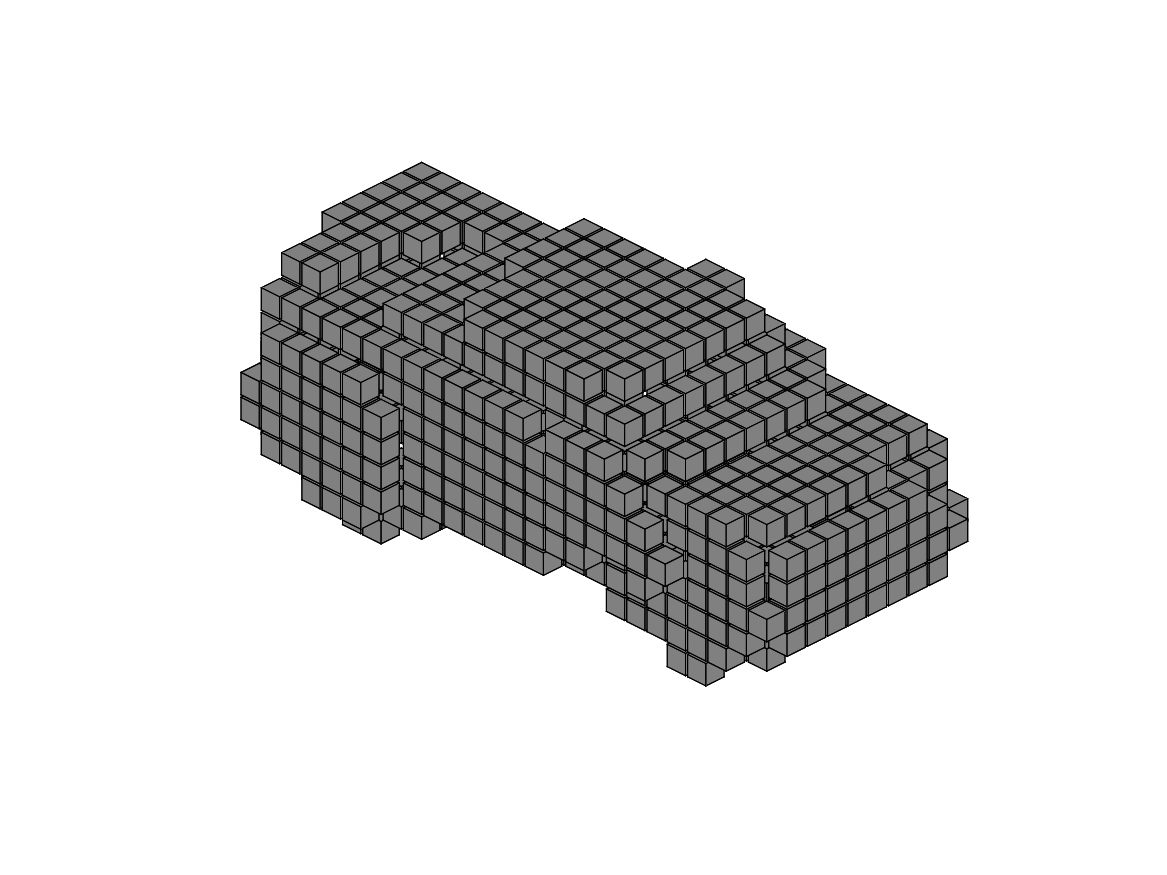
\includegraphics[height=1.5cm,trim={3cm 2cm 3cm 2cm},clip]{images/0_prediction_45}
      };
      
      \node at (4.7, 0) {\footnotesize Decoder};
      \draw[-] ($(output.north west) - (0.25,0)$) -- (3.75,0.5);
      \draw[-] ($(output.south west) - (0.25,0)$) -- (3.75,-0.5);
      \draw[-] ($(output.south west) - (0.25,0)$) -- ($(output.north west) - (0.25,0)$);
      \draw[-] (3.75,-0.5) -- (3.75,0.5);
      
      \node (ry) at (8.5, 0) {\footnotesize $\tilde{y}$};
      
      \node[color=RWTHdarkorange] at (0.5,1.4) {\footnotesize Recognition Model $q(z|y)$};
      \node[rectangle,dashed,draw=RWTHdarkorange,minimum width=5.2cm,minimum height=3cm] at (0.7, 0.25) {};
      
      \node[color=RWTHgreen] at (6,1.4) {\footnotesize Generative Model $p(y|z) p(z)$};
      \node[rectangle,dashed,draw=RWTHgreen,minimum width=5.5cm,minimum height=3cm] at (6.1, 0.25) {};
      
      \node[] (L) at (3.5, -2) {\footnotesize Reconstruction and Prior Loss};
          
      \draw[-] (ry) -- ($(ry) - (0,2)$);
      \draw[-] ($(ry) - (0,2)$) -- (L);
      \draw[-] (y) -- ($(y) - (0,2)$);
      \draw[-] ($(y) - (0,2)$) -- (L);
    \end{tikzpicture}
  \end{frame}
  
  \begin{frame}
    {\large Proposed Approach}
    
    \textbf{Shape inference.}\\[6px]
    Perform maximum likelihood:
    
    \vspace{0.5cm}
    \begin{tikzpicture}
      \node[transparent] (y) at (-1.5, 0) {\footnotesize $y$};
          
      \node[transparent,rectangle,draw=black] (input) at (0, 0) {
        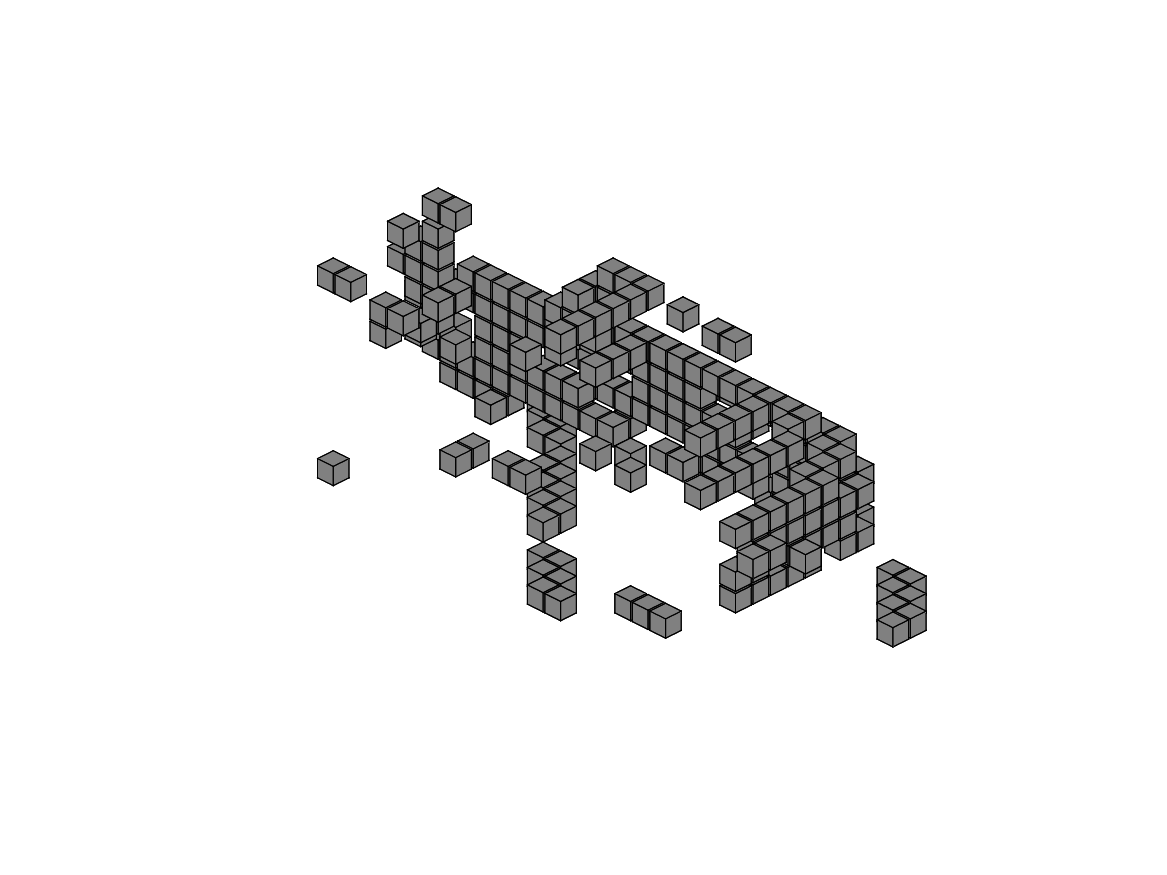
\includegraphics[height=1.5cm,trim={3cm 2cm 3cm 2cm},clip]{images/0_input_45}
      };
      
      \node[transparent] at (2.3, 0) {\footnotesize Encoder};
      \draw[transparent,-] ($(input.north east) + (0.25,0)$) -- (3.25,0.5);
      \draw[transparent,-] ($(input.south east) + (0.25,0)$) -- (3.25,-0.5);
      \draw[transparent,-] ($(input.south east) + (0.25,0)$) -- ($(input.north east) + (0.25,0)$);
      \draw[transparent,-] (3.25,-0.5) -- (3.25,0.5);
      
      \node (z) at (3.5, 0) {\footnotesize $z$};
      
      \node[rectangle,draw=black] (output) at (7, 0) {
        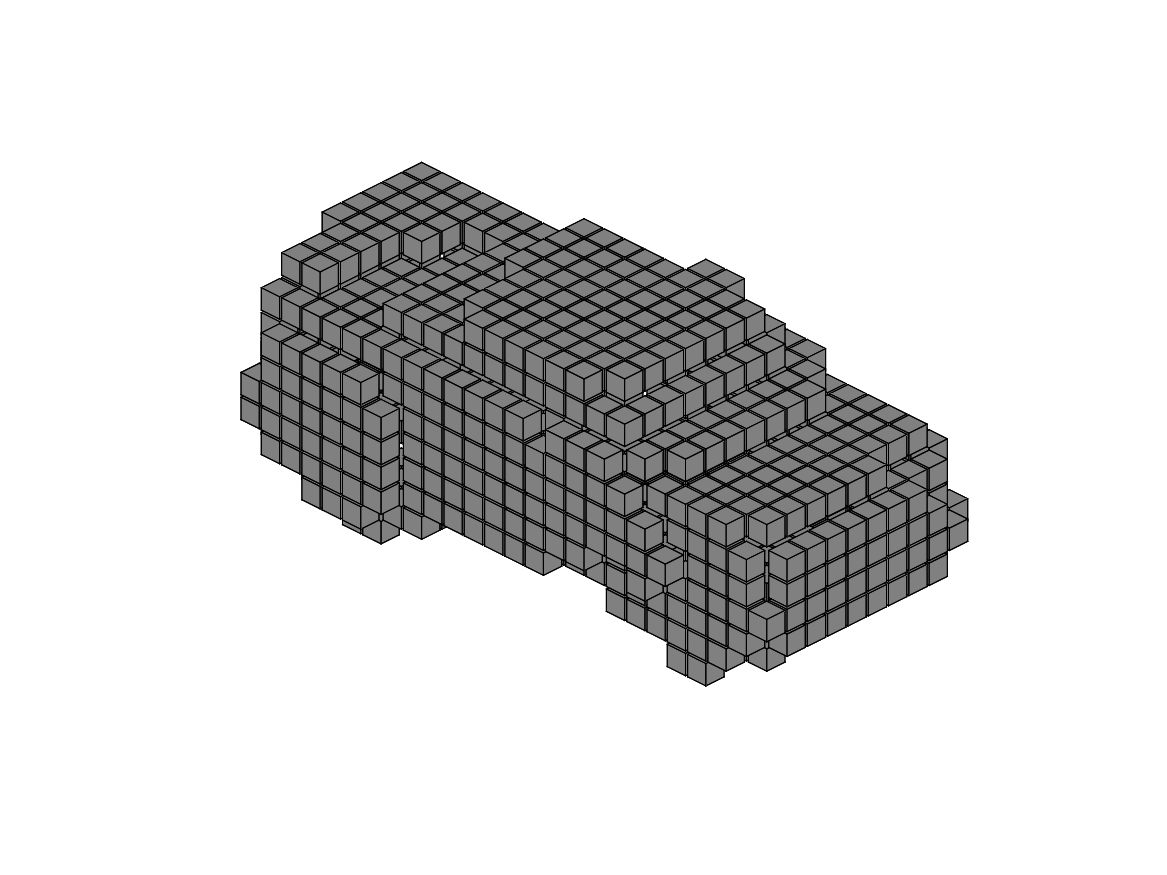
\includegraphics[height=1.5cm,trim={3cm 2cm 3cm 2cm},clip]{images/0_prediction_45}
      };
      
      \node at (4.7, 0) {\footnotesize Decoder};
      \draw[-] ($(output.north west) - (0.25,0)$) -- (3.75,0.5);
      \draw[-] ($(output.south west) - (0.25,0)$) -- (3.75,-0.5);
      \draw[-] ($(output.south west) - (0.25,0)$) -- ($(output.north west) - (0.25,0)$);
      \draw[-] (3.75,-0.5) -- (3.75,0.5);
      
      \node (ry) at (8.5, 0) {\footnotesize $\tilde{y}$};
      
      \node[transparent,color=RWTHdarkorange] at (0.5,1.4) {\footnotesize Recognition Model $q(z|y)$};
      \node[transparent,rectangle,dashed,draw=RWTHdarkorange,minimum width=5.2cm,minimum height=3cm] at (0.7, 0.25) {};
      
      \node[color=RWTHgreen] at (6,1.4) {\footnotesize Generative Model $p(y|z) p(z)$};
      \node[rectangle,dashed,draw=RWTHgreen,minimum width=5.5cm,minimum height=3cm] at (6.1, 0.25) {};
      
      \node[transparent] (L) at (3.5, -2) {\footnotesize \begin{tabular}{c}\textbf{Unsupervised}\\Maximum Likelihood Loss\end{tabular}};
          
      \draw[transparent,-] (ry) -- ($(ry) - (0,2)$);
      \draw[transparent,-] ($(ry) - (0,2)$) -- (L);
      \draw[transparent,-] (y) -- ($(y) - (0,2)$);
      \draw[transparent,-] ($(y) - (0,2)$) -- (L);
    \end{tikzpicture}
  \end{frame}
  
  \begin{frame}
    {\large Proposed Approach}
    
    \textbf{Shape inference.}\\[6px]
    Perform maximum likelihood:
    
    \vspace{0.5cm}
    \begin{tikzpicture}
      \node[] (y) at (-1.5, 0) {\footnotesize $x$};
          
      \node[rectangle,draw=black] (input) at (0, 0) {
        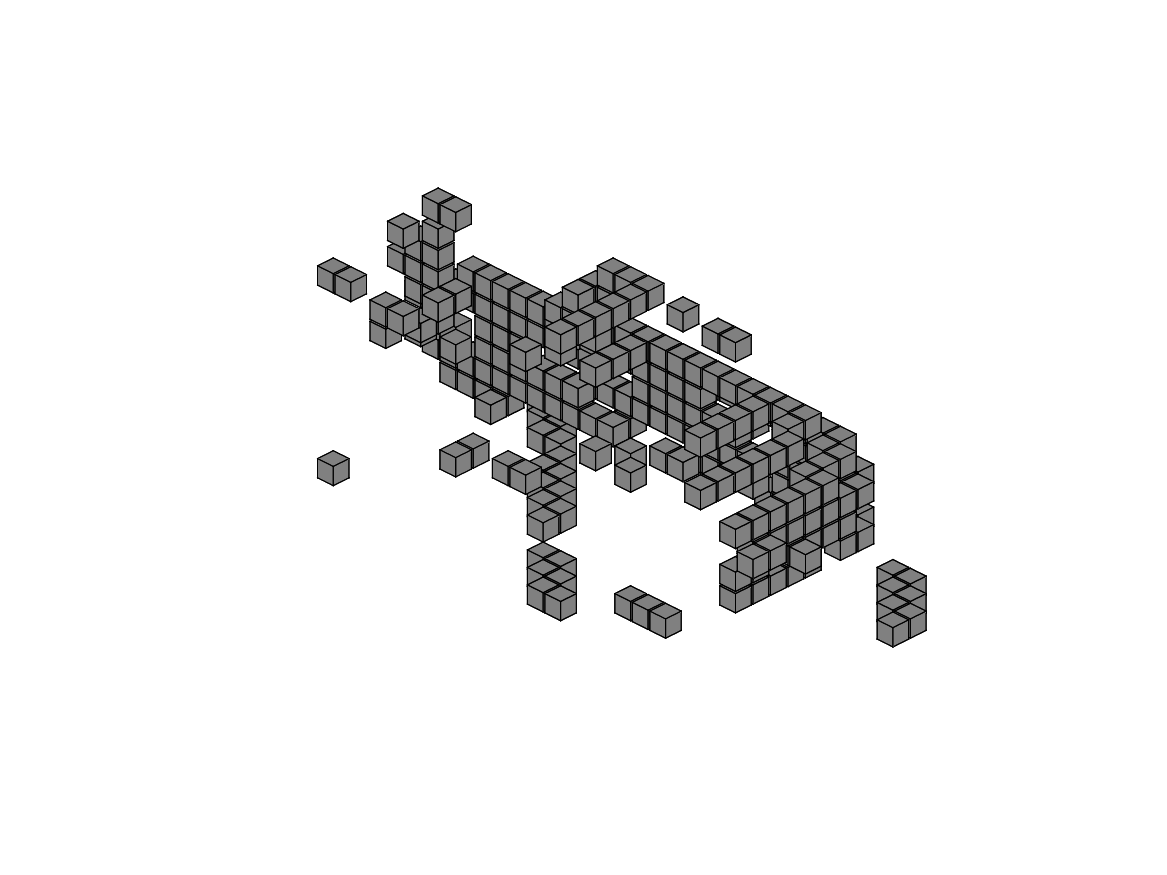
\includegraphics[height=1.5cm,trim={3cm 2cm 3cm 2cm},clip]{images/0_input_45}
      };
      
      \node[transparent] at (2.3, 0) {\footnotesize Encoder};
      \draw[transparent,-] ($(input.north east) + (0.25,0)$) -- (3.25,0.5);
      \draw[transparent,-] ($(input.south east) + (0.25,0)$) -- (3.25,-0.5);
      \draw[transparent,-] ($(input.south east) + (0.25,0)$) -- ($(input.north east) + (0.25,0)$);
      \draw[transparent,-] (3.25,-0.5) -- (3.25,0.5);
      
      \node (z) at (3.5, 0) {\footnotesize $z$};
      
      \node[rectangle,draw=black] (output) at (7, 0) {
        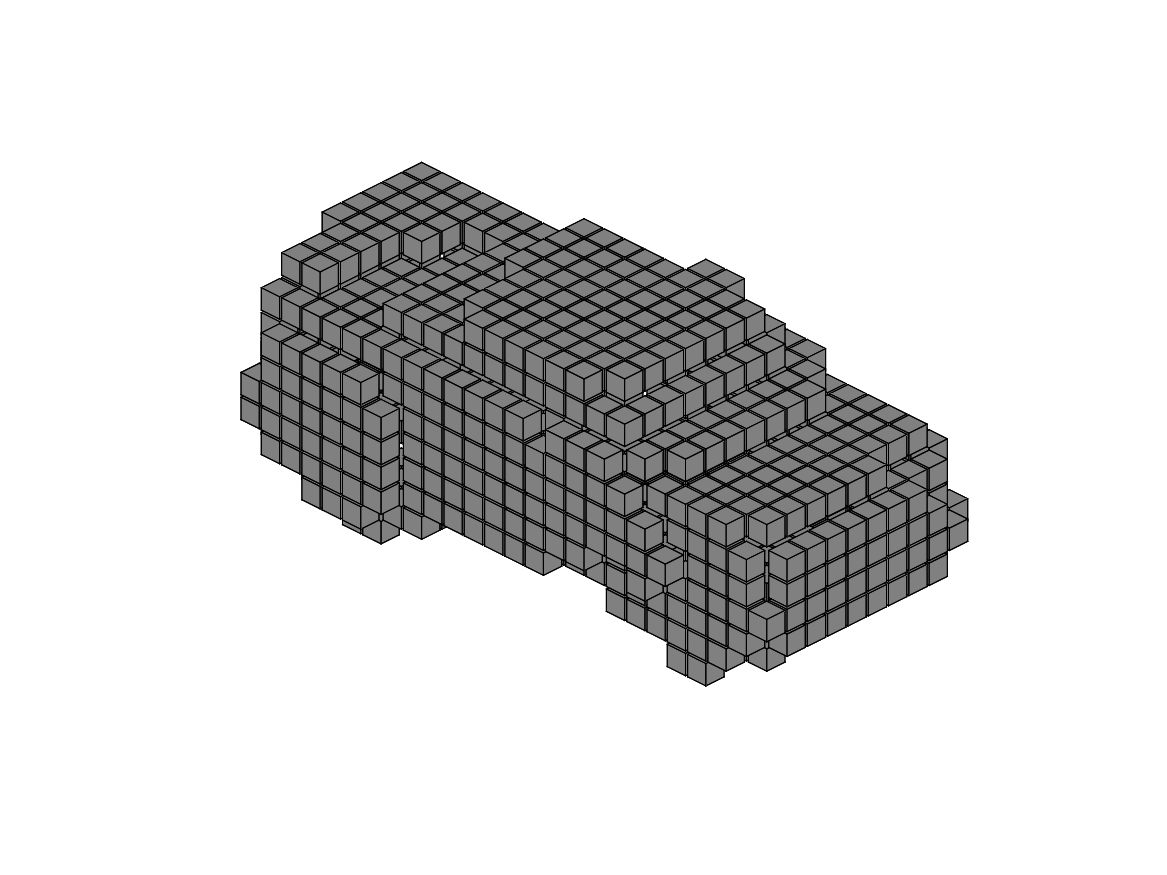
\includegraphics[height=1.5cm,trim={3cm 2cm 3cm 2cm},clip]{images/0_prediction_45}
      };
      
      \node at (4.7, 0) {\footnotesize Decoder};
      \draw[-] ($(output.north west) - (0.25,0)$) -- (3.75,0.5);
      \draw[-] ($(output.south west) - (0.25,0)$) -- (3.75,-0.5);
      \draw[-] ($(output.south west) - (0.25,0)$) -- ($(output.north west) - (0.25,0)$);
      \draw[-] (3.75,-0.5) -- (3.75,0.5);
      
      \node (ry) at (8.5, 0) {\footnotesize $\tilde{y}$};
      
      \node[transparent,color=RWTHdarkorange] at (0.5,1.4) {\footnotesize Recognition Model $q(z|y)$};
      \node[transparent,rectangle,dashed,draw=RWTHdarkorange,minimum width=5.2cm,minimum height=3cm] at (0.7, 0.25) {};
      
      \node[color=RWTHgreen] at (6,1.4) {\footnotesize Generative Model $p(y|z) p(z)$};
      \node[rectangle,dashed,draw=RWTHgreen,minimum width=5.5cm,minimum height=3cm] at (6.1, 0.25) {};
      
      \node[] (L) at (3.5, -2) {\footnotesize Maximum Likelihood};
          
      \draw[-] (ry) -- ($(ry) - (0,2)$);
      \draw[-] ($(ry) - (0,2)$) -- (L);
      \draw[-] (y) -- ($(y) - (0,2)$);
      \draw[-] ($(y) - (0,2)$) -- (L);
    \end{tikzpicture}
  \end{frame}
  
  \begin{frame}
    {\large Proposed Approach}
    
    \textbf{Shape inference.}\\[6px]
    \st{Perform} Learn -- \ie amortize -- maximum likelihood:
    
    \vspace{0.5cm}
    \begin{tikzpicture}
      \node[] (y) at (-1.5, 0) {\footnotesize $x$};
          
      \node[rectangle,draw=black] (input) at (0, 0) {
        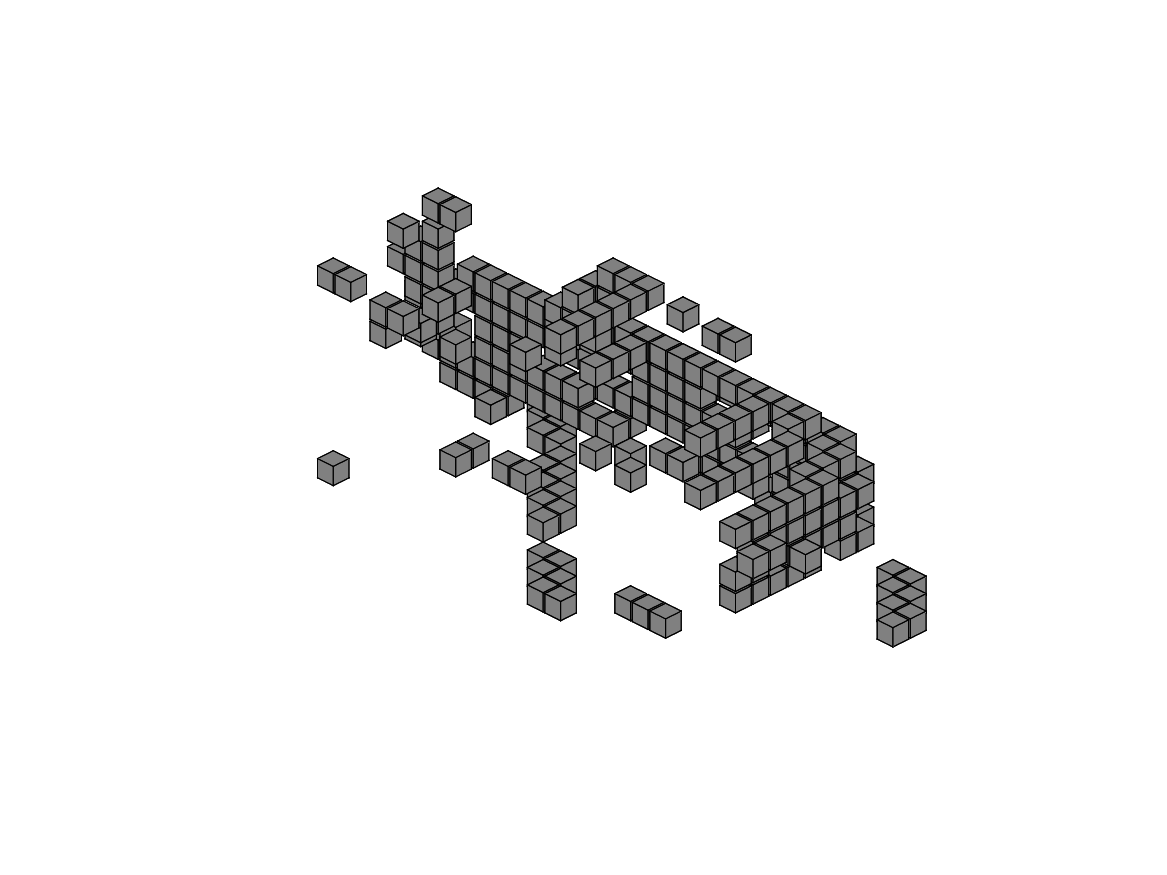
\includegraphics[height=1.5cm,trim={3cm 2cm 3cm 2cm},clip]{images/0_input_45}
      };
      
      \node[] at (2.3, 0) {\footnotesize Encoder};
      \draw[-] ($(input.north east) + (0.25,0)$) -- (3.25,0.5);
      \draw[-] ($(input.south east) + (0.25,0)$) -- (3.25,-0.5);
      \draw[-] ($(input.south east) + (0.25,0)$) -- ($(input.north east) + (0.25,0)$);
      \draw[-] (3.25,-0.5) -- (3.25,0.5);
      
      \node (z) at (3.5, 0) {\footnotesize $z$};
      
      \node[rectangle,draw=black] (output) at (7, 0) {
        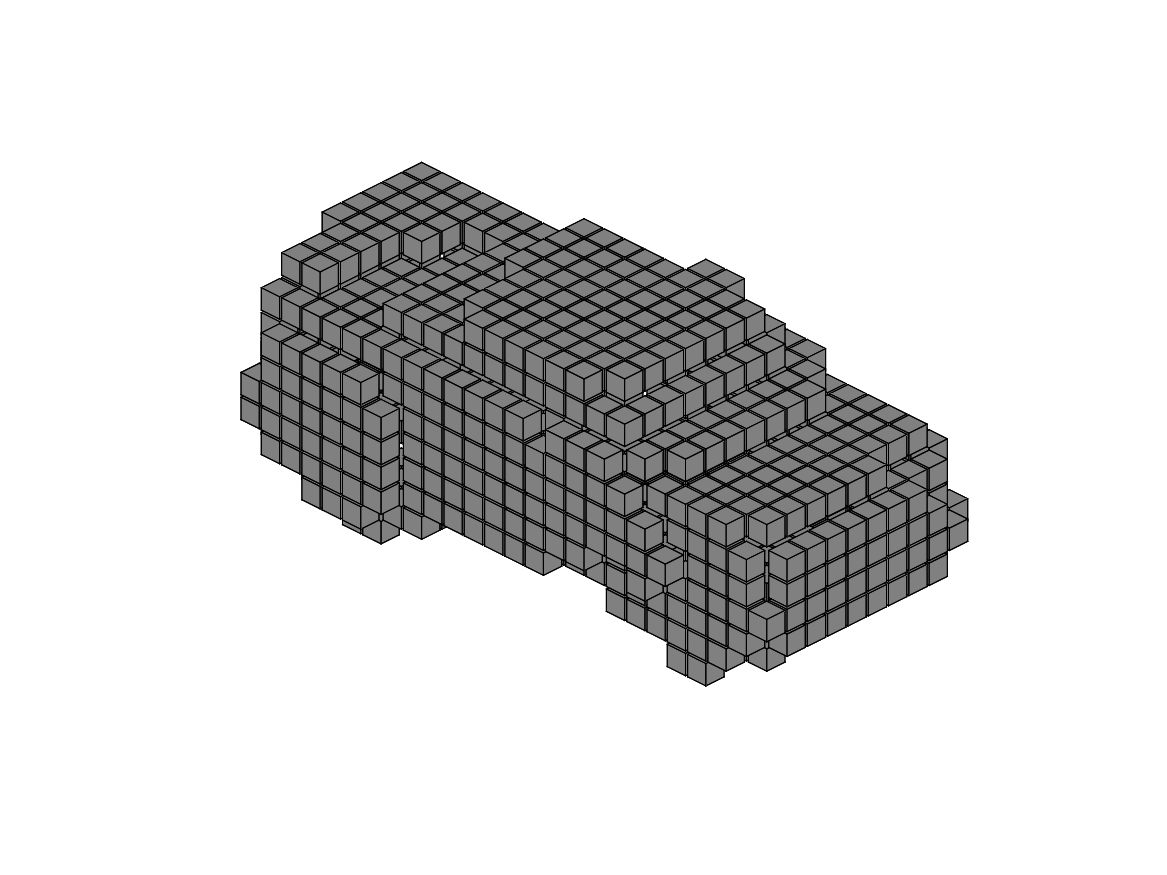
\includegraphics[height=1.5cm,trim={3cm 2cm 3cm 2cm},clip]{images/0_prediction_45}
      };
      
      \node at (4.7, 0) {\footnotesize Decoder};
      \draw[-] ($(output.north west) - (0.25,0)$) -- (3.75,0.5);
      \draw[-] ($(output.south west) - (0.25,0)$) -- (3.75,-0.5);
      \draw[-] ($(output.south west) - (0.25,0)$) -- ($(output.north west) - (0.25,0)$);
      \draw[-] (3.75,-0.5) -- (3.75,0.5);
      
      \node (ry) at (8.5, 0) {\footnotesize $\tilde{y}$};
      
      \node[color=RWTHdarkorange] at (-0.2,1.4) {\footnotesize Deterministic $z(x)$};
      \node[rectangle,dashed,draw=RWTHdarkorange,minimum width=5.2cm,minimum height=3cm] at (0.7, 0.25) {};
      
      \node[color=RWTHgreen] at (6,1.4) {\footnotesize Generative Model $p(y|z) p(z)$};
      \node[rectangle,dashed,draw=RWTHgreen,minimum width=5.5cm,minimum height=3cm] at (6.1, 0.25) {};
      
      \node[] (L) at (3.5, -2) {\footnotesize \begin{tabular}{c}Unsupervised\\Maximum Likelihood Loss\end{tabular}};
          
      \draw[-] (ry) -- ($(ry) - (0,2)$);
      \draw[-] ($(ry) - (0,2)$) -- (L);
      \draw[-] (y) -- ($(y) - (0,2)$);
      \draw[-] ($(y) - (0,2)$) -- (L);
    \end{tikzpicture}
  \end{frame}
  
  \begin{frame}[plain,noframenumbering]
    \begin{center}
      {\Large Shape Prior}
    \end{center}
  \end{frame}
  
  \begin{frame}
    {\large Shape Prior}
    
    Learn a variational auto-encoder:
    \vspace{-0.25cm}
    
    \begin{figure}
      \centering
      \begin{subfigure}[t]{0.415\textwidth}
        \vspace*{-0.25cm}
        \hspace*{-0.45cm}
        \begin{tikzpicture}
          \tikzstyle{state}=[circle,draw=RWTHblack,thick,minimum size=1.25cm];
          \node[state] at (0,0) (x) {$y$};
          \node[state] at (0,3) (z) {$z$};
          \draw[arrow] (x) to[out=110,in=250] (z);
          \draw[arrow] (z) to[out=290,in=70] (x);
          \node at (-1.5,1.5) { $q(z|y)$};
          \node at (1.5,1.5) {$p(y|z)$};
          \node at (0,4.2) {$p(z)$};
        \end{tikzpicture}
      \end{subfigure}
      \begin{subfigure}[t]{0.56\textwidth}
        \vspace{0.15cm}
        
        \hphantom{Prior $p(z) = \mathcal{N}(z|0,I)$}
        \vspace{0.25cm}
        
        \hphantom{{\color{RWTHgreen} Decoder/Generative Model}}
        \hphantom{\hfill\hspace*{0.5cm}{\color{RWTHgreen} $p(y|z) = \prod_i \text{Ber}(y_i | \theta_i(z))$}\hfill}
        \vspace{0.25cm}
        
        \hphantom{{\color{RWTHdarkorange} Encoder/Recognition Model}}
        \hphantom{\hfill\hspace*{0.5cm}{\color{RWTHdarkorange} $q(z|y) = \mathcal{N}(z|\mu(y), \sigma^2(y))$}\hfill}
      \end{subfigure}
    \end{figure}
  \end{frame}
  
  \begin{frame}
    {\large Shape Prior}
    
    Learn a variational auto-encoder:
    \vspace{-0.25cm}
    
    \begin{figure}
      \centering
      \begin{subfigure}[t]{0.415\textwidth}
        \vspace*{-0.25cm}
        \hspace*{-0.45cm}
        \begin{tikzpicture}
          \tikzstyle{state}=[circle,draw=RWTHblack,thick,minimum size=1.25cm];
          \node[state] at (0,0) (x) {$y$};
          \node[state] at (0,3) (z) {$z$};
          \draw[arrow] (x) to[out=110,in=250] (z);
          \draw[arrow] (z) to[out=290,in=70] (x);
          \node at (-1.5,1.5) { $q(z|y)$};
          \node at (1.5,1.5) {$p(y|z)$};
          \node at (0,4.2) {$p(z)$};
        \end{tikzpicture}
      \end{subfigure}
      \begin{subfigure}[t]{0.56\textwidth}
        \vspace{0.15cm}
        Prior $p(z) = \mathcal{N}(z|0,I)$
      \end{subfigure}
    \end{figure}
  \end{frame}
  
  \begin{frame}
    {\large Shape Prior}
    
    Learn a variational auto-encoder:
    \vspace{-0.25cm}
    
    \begin{figure}
      \centering
      \begin{subfigure}[t]{0.415\textwidth}
        \vspace*{-0.25cm}
        \hspace*{-0.45cm}
        \begin{tikzpicture}
          \tikzstyle{state}=[circle,draw=RWTHblack,thick,minimum size=1.25cm];
          \node[state] at (0,0) (x) {$y$};
          \node[state] at (0,3) (z) {$z$};
          \draw[arrow] (x) to[out=110,in=250] (z);
          \draw[arrow,RWTHgreen] (z) to[out=290,in=70] (x);
          \node at (-1.5,1.5) {$q(z|y)$};
          \node at (1.5,1.5) {\color{RWTHgreen}$p(y|z)$};

          \node at (0,4.2) {$p(z)$};
        \end{tikzpicture}
      \end{subfigure}
      \begin{subfigure}[t]{0.56\textwidth}
        \vspace{0.15cm}
        Prior $p(z) = \mathcal{N}(z|0,I)$
        \vspace{0.25cm}
        
        {\color{RWTHgreen} Decoder/Generative Model}\\[4px]
        \hfill\hspace*{0.5cm}{\color{RWTHgreen} $p(y|z) = \prod_i \text{Ber}(y_i | \theta_i(z))$}\hfill
      \end{subfigure}
    \end{figure}
  \end{frame}
  
  \begin{frame}
    {\large Shape Prior}
    
    Learn a variational auto-encoder:
    
    \begin{figure}
      \centering
      \begin{subfigure}[t]{0.415\textwidth}
        %\begin{mdframed}
          \vspace*{-0.25cm}
          \hspace*{-0.45cm}
          \begin{tikzpicture}
            \tikzstyle{state}=[circle,draw=RWTHblack,thick,minimum size=1.25cm];
            \node[state] at (0,0) (x) {$y$};
            \node[state] at (0,3) (z) {$z$};
            \draw[arrow,RWTHdarkorange] (x) to[out=110,in=250] (z);
            \draw[arrow,RWTHgreen] (z) to[out=290,in=70] (x);
            \node at (-1.5,1.5) {\color{RWTHdarkorange} $q(z|y)$};
            \node at (1.5,1.5) {\color{RWTHgreen} $p(y|z)$};
            \node at (0,4.2) {$p(z)$};
          \end{tikzpicture}
        %\end{mdframed}
      \end{subfigure}
      \begin{subfigure}[t]{0.56\textwidth}
        \vspace{0.15cm}
        Prior $p(z) = \mathcal{N}(z|0,I)$
        \vspace{0.25cm}
        
        {\color{RWTHgreen} Decoder/Generative Model}\\[4px]
        \hfill\hspace*{0.5cm}{\color{RWTHgreen} $p(y|z) = \prod_i \text{Ber}(y_i | \theta_i(z))$}\hfill
        \vspace{0.25cm}
        
        {\color{RWTHdarkorange} Encoder/Recognition Model}\\[4px]
        \hfill\hspace*{0.5cm}{\color{RWTHdarkorange} $q(z|y) = \mathcal{N}(z|\mu(y), \sigma^2(y))$}\hfill
      \end{subfigure}
    \end{figure}
  \end{frame}
  
  \begin{frame}
    {\large Shape Prior}
    
    Maximum likelihood leads to:
    \vspace{-0.25cm}
    
    \begin{align}
      \mathcal{L}_{\text{ELBO}} &=- \mathbb{E}_{q(z|y)}[\log p(y|z)] + \text{KL}(q(z|y)|p(z))\notag
    \end{align}
    \only<1-2>{\tikz[overlay]{
      \draw[arrow,transparent] (9.15,2.15) node{reconstruction} (7.4,2.2) [out=170,in=45]to (5,1.65);
      \only<2>{\draw[arrow,RWTHblue] (5,0.4) node{prior} (5.7, 0.35) [out=350,in=215]to (9,1);}
    }}
    
    \begin{itemize}
      \item Encoder: $q(z | y) = \mathcal{N}(z | \mu(y), \sigma^2(y))$;
      \item and decoder: $p(y | z) = \prod_i \text{Ber}(y_i | \theta_i(z))$.
    \end{itemize}
  \end{frame}
  
  \begin{frame}
    {\large Shape Prior}
    
    Maximum likelihood leads to:
    \vspace{-0.25cm}
    
    \begin{align}
      \mathcal{L}_{\text{ELBO}} &= - \mathbb{E}_{q(z|y)}[\log p(y|z)] + {\color{RWTHred}\mathcal{P}_{\text{Reg}}(\mu(y), \sigma^2(y))}\notag
    \end{align}
    \only<1-2>{\tikz[overlay]{
      \only<2>{\draw[arrow,RWTHblue] (9.15,2.15) node{reconstruction} (7.4,2.2) [out=170,in=45]to (5,1.65);}
      \draw[arrow,transparent] (5,0.4) node{prior} (5.7, 0.35) [out=350,in=215]to (9,1);
    }}
    
    \begin{itemize}
      \item Encoder: $q(z | y) = \mathcal{N}(z | \mu(y), \sigma^2(y))$;
      \item and decoder: $p(y | z) = \prod_i \text{Ber}(y_i | \theta_i(z))$.
    \end{itemize}
  \end{frame}
  
  \begin{frame}
    {\large Shape Prior}
    
    Maximum likelihood leads to:
    \vspace{-0.25cm}
    
    \begin{align}
      \mathcal{L}_{\text{ELBO}} &= {\color{RWTHred}\sum_i \mathcal{L}_{\text{BCE}}(\tilde{y}_i, y_i)} + \mathcal{P}_{\text{Reg}}(\mu(y), \sigma^2(y))\notag
    \end{align}
    \tikz[overlay]{
      \node[rotate=90] at (5.25, 0.75) {\color{RWTHred}$\hat{=}$};
      \node at (5.25,0.25) {\color{RWTHred}$\theta_i(z)$};
      \draw[arrow,transparent] (9.15,2.15) node{reconstruction} (7.4,2.2) [out=170,in=45]to (5,1.65);
      \draw[arrow,transparent] (5,0.4) node{prior} (5.7, 0.35) [out=350,in=215]to (9,1);
    }
    
    \begin{itemize}
      \item Encoder: $q(z | y) = \mathcal{N}(z | \mu(y), \sigma^2(y))$;
      \item and decoder: $p(y | z) = \prod_i \text{Ber}(y_i | \theta_i(z))$.
    \end{itemize}
  \end{frame}
  
  \begin{frame}
    {\large Shape Prior}
    
    Maximum likelihood leads to:
    \vspace{-0.25cm}
    
    \begin{align}
      \color{RWTHred}\mathcal{L}(\tilde{y}, y) &= \sum_i \mathcal{L}_{\text{BCE}}(\tilde{y}_i, y_i) + \mathcal{P}_{\text{Reg}}(\mu(y), \sigma^2(y))\notag
    \end{align}
    \tikz[overlay]{
      \draw[arrow,transparent] (9.15,2.15) node{reconstruction} (7.4,2.2) [out=170,in=45]to (5,1.65);
      \draw[arrow,transparent] (5,0.4) node{prior} (5.7, 0.35) [out=350,in=215]to (9,1);
    }
    
    \begin{itemize}
      \item Encoder: $q(z | y) = \mathcal{N}(z | \mu(y), \sigma^2(y))$;
      \item and decoder: $p(y | z) = \prod_i \text{Ber}(y_i | \theta_i(z))$.
    \end{itemize}
  \end{frame}
  
  \begin{frame}
    {\large Shape Prior}
    
      Training a variational auto-encoder:
      \begin{center}
        \begin{tikzpicture}
          \node (y) at (-1.5, 0) {\footnotesize $y$};
          
          \node[rectangle,draw=RWTHorange] (input) at (0, 0) {
            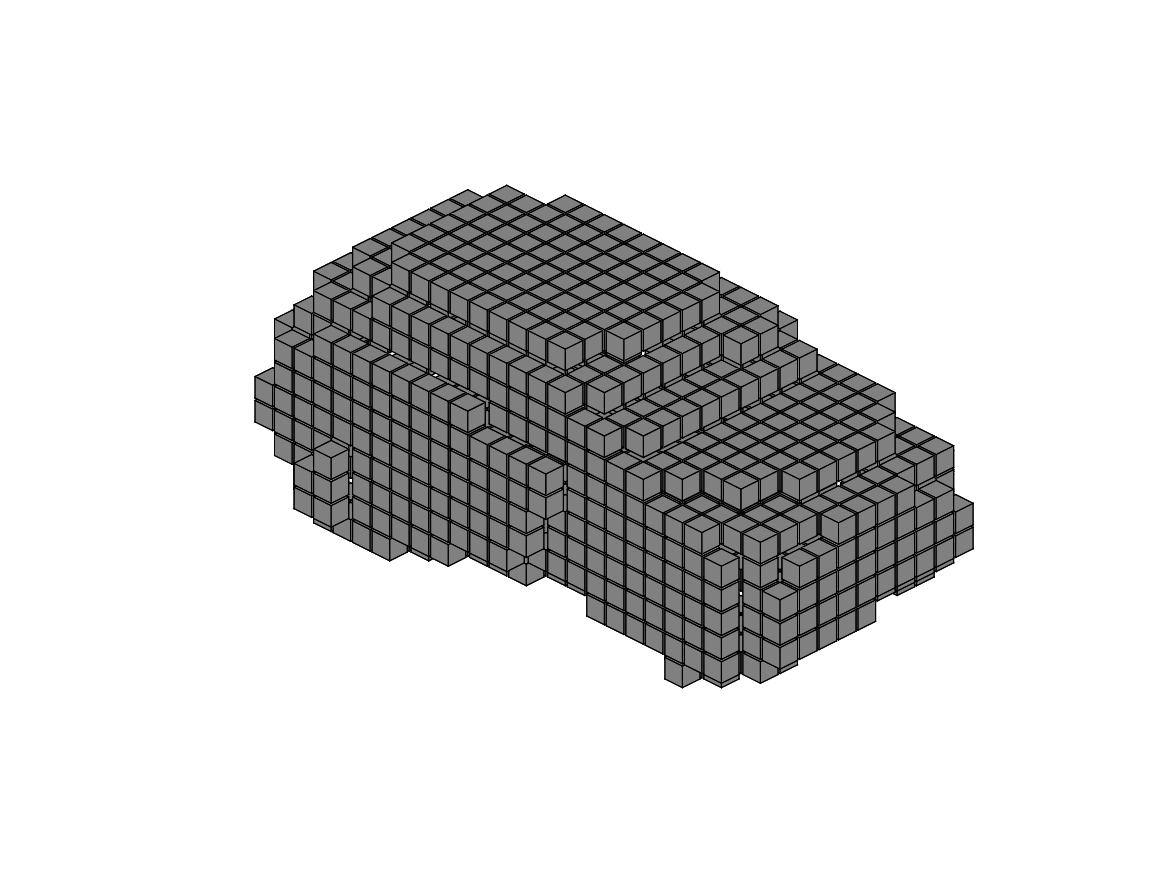
\includegraphics[height=1.5cm,trim={3cm 2cm 3cm 2cm},clip]{images/0_baseline_prediction_45}
          };
          
          \node[RWTHdarkorange] at (2.25, 0) {\footnotesize $q(z|y)$};
          \draw[RWTHdarkorange,-] ($(input.north east) + (0.25,0)$) -- (3,0.5);
          \draw[RWTHdarkorange,-] ($(input.south east) + (0.25,0)$) -- (3,-0.5);
          \draw[RWTHdarkorange,-] ($(input.south east) + (0.25,0)$) -- ($(input.north east) + (0.25,0)$);
          \draw[RWTHdarkorange,-] (3,-0.5) -- (3,0.5);
          
          \node (z) at (3.5, 0) {\footnotesize $z$};
          
          \node[rectangle,draw=RWTHgreen] (output) at (7, 0) {
            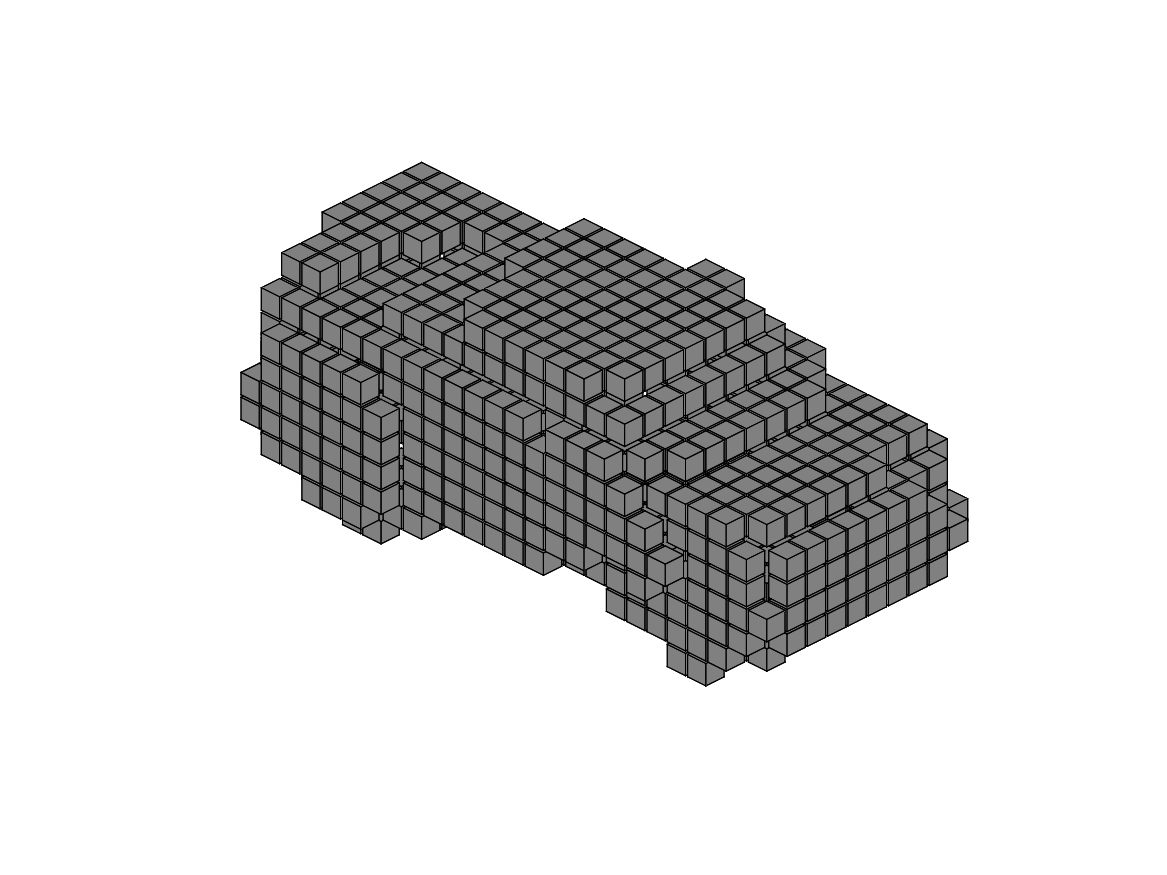
\includegraphics[height=1.5cm,trim={3cm 2cm 3cm 2cm},clip]{images/0_prediction_45}
          };
          
          \node[RWTHgreen] at (4.75, 0) {\footnotesize $p(y|z)$};
          \draw[RWTHgreen,-] ($(output.north west) - (0.25,0)$) -- (4,0.5);
          \draw[RWTHgreen,-] ($(output.south west) - (0.25,0)$) -- (4,-0.5);
          \draw[RWTHgreen,-] ($(output.south west) - (0.25,0)$) -- ($(output.north west) - (0.25,0)$);
          \draw[RWTHgreen,-] (4,-0.5) -- (4,0.5);
          
          \node (ry) at (8.5, 0) {\footnotesize $\tilde{y}$};
          
          \node (L) at (3.5, -2) {\footnotesize \begin{tabular}{c}Reconstruction and Prior Loss\\$\mathcal{L}(\tilde{y}, y)$\end{tabular}};
              
          \draw[-] (ry) -- ($(ry) - (0,2)$);
          \draw[-] ($(ry) - (0,2)$) -- (L);
          \draw[-] (y) -- ($(y) - (0,2)$);
          \draw[-] ($(y) - (0,2)$) -- (L);
        \end{tikzpicture}
      \end{center}
      Generating random shapes:
      
      \begin{center}
        \begin{tikzpicture}
          \node at (0, 0) {
            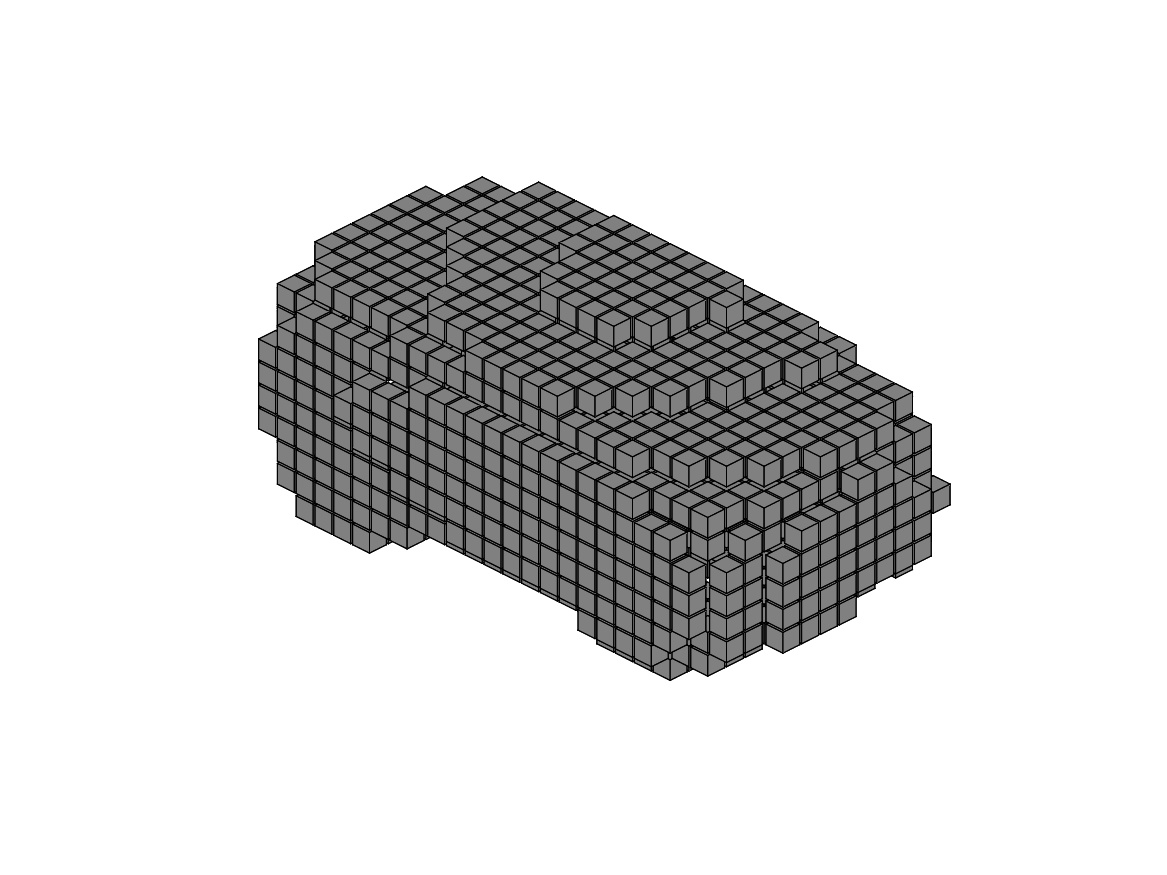
\includegraphics[width=2cm,trim={3cm 2cm 3cm 2cm},clip]{../thesis/images/experiments/shapenet/vae_occ/easy_15_long/0_random_45}
          };
          \node at (2, 0) {
            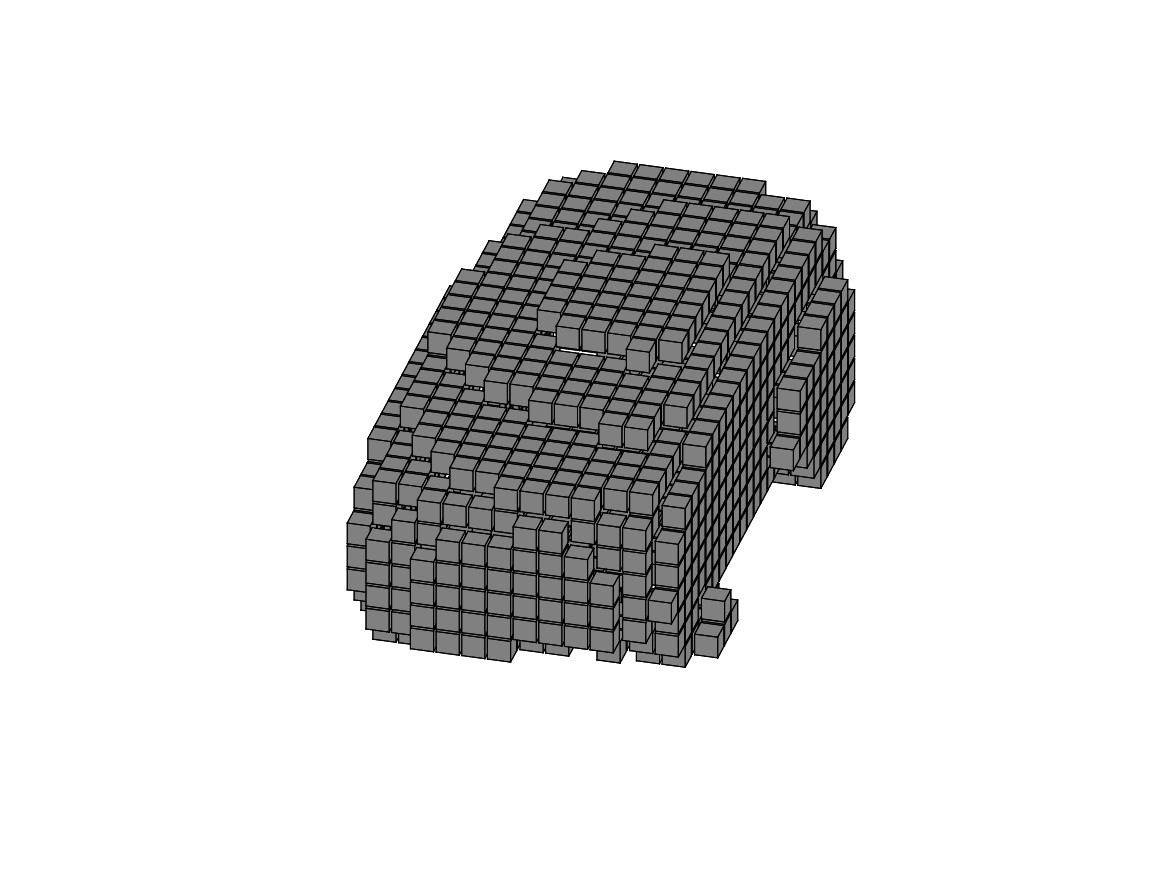
\includegraphics[width=2cm,trim={3cm 2cm 3cm 2cm},clip]{../thesis/images/experiments/shapenet/vae_occ/easy_15_long/0_random_105}
          };
          
          \draw[-,dashed] (3.25, -1) -- (3.25, 1);
          
          \node at (4.5, 0) {
            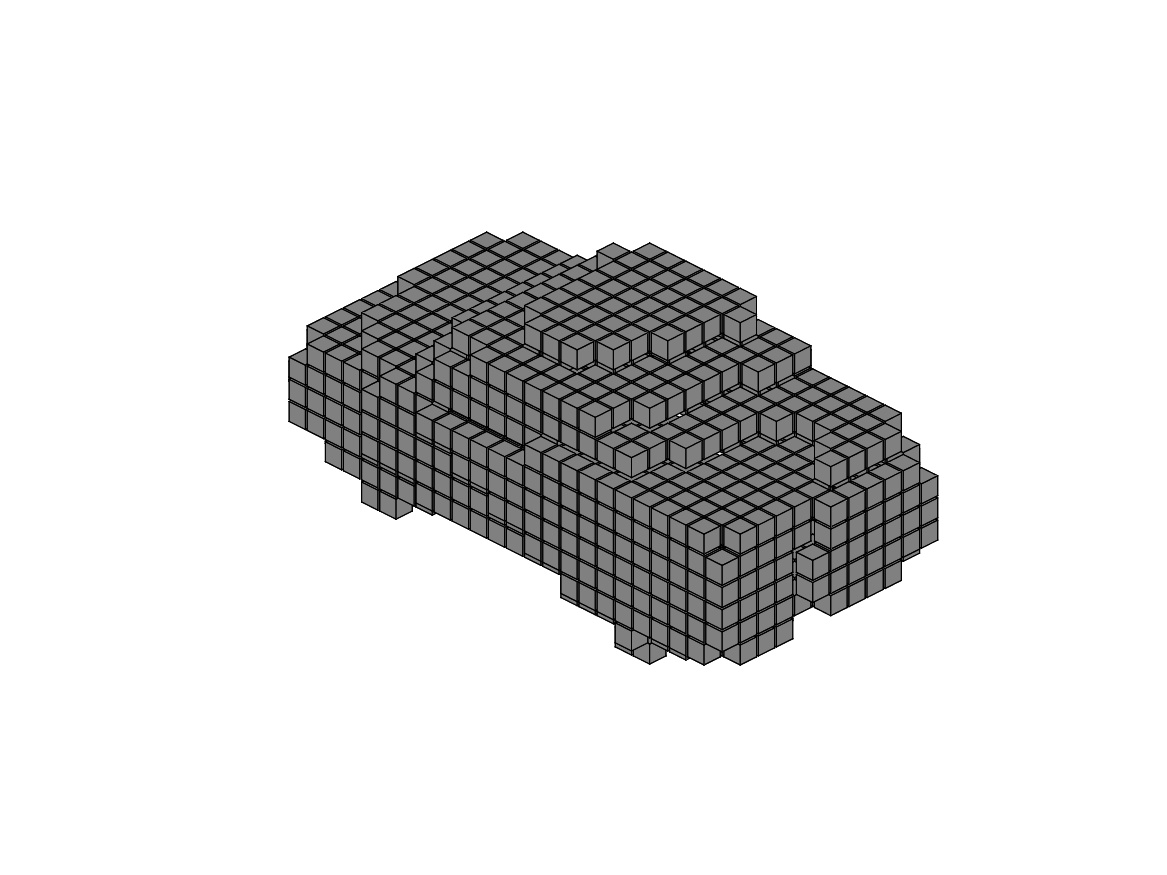
\includegraphics[width=2cm,trim={3cm 2cm 3cm 2cm},clip]{../thesis/images/experiments/shapenet/vae_occ/easy_15_long/1_random_45}
          };
          \node at (6.5, 0) {
            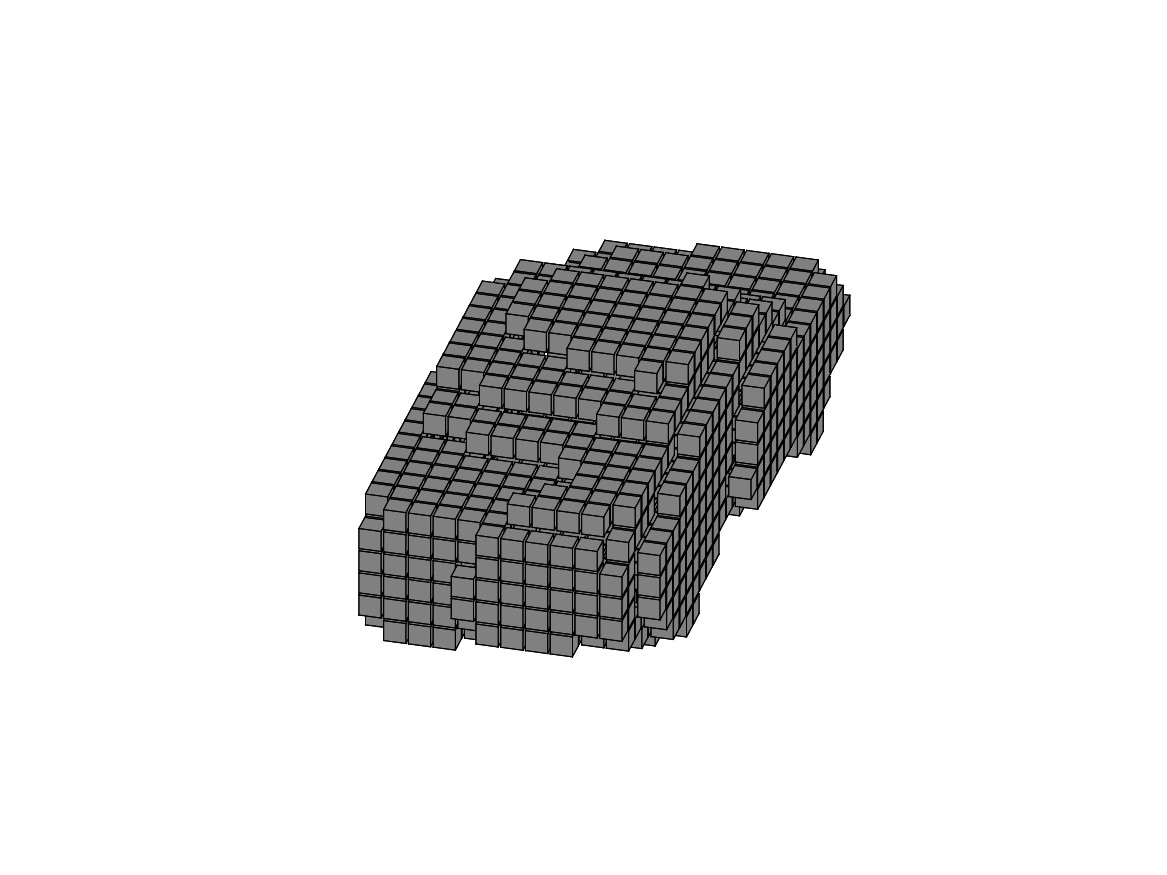
\includegraphics[width=2cm,trim={3cm 2cm 3cm 2cm},clip]{../thesis/images/experiments/shapenet/vae_occ/easy_15_long/1_random_105}
          };
        \end{tikzpicture}
      \end{center}
  \end{frame}
  
  \begin{frame}[plain,noframenumbering]
    \begin{center}
      {\Large Shape Inference}
    \end{center}
  \end{frame}
  
  \begin{frame}[t]
    {\large Shape Inference}
    
    Maximize the likelihood of observation $x$ over the latent space:
    \begin{center}
      {\setbeamercovered{transparent}
      \begin{tikzpicture}
        \node[] (y) at (-1.5, 0) {\footnotesize $x$};
            
        \node[rectangle,draw=black] (input) at (0, 0) {
          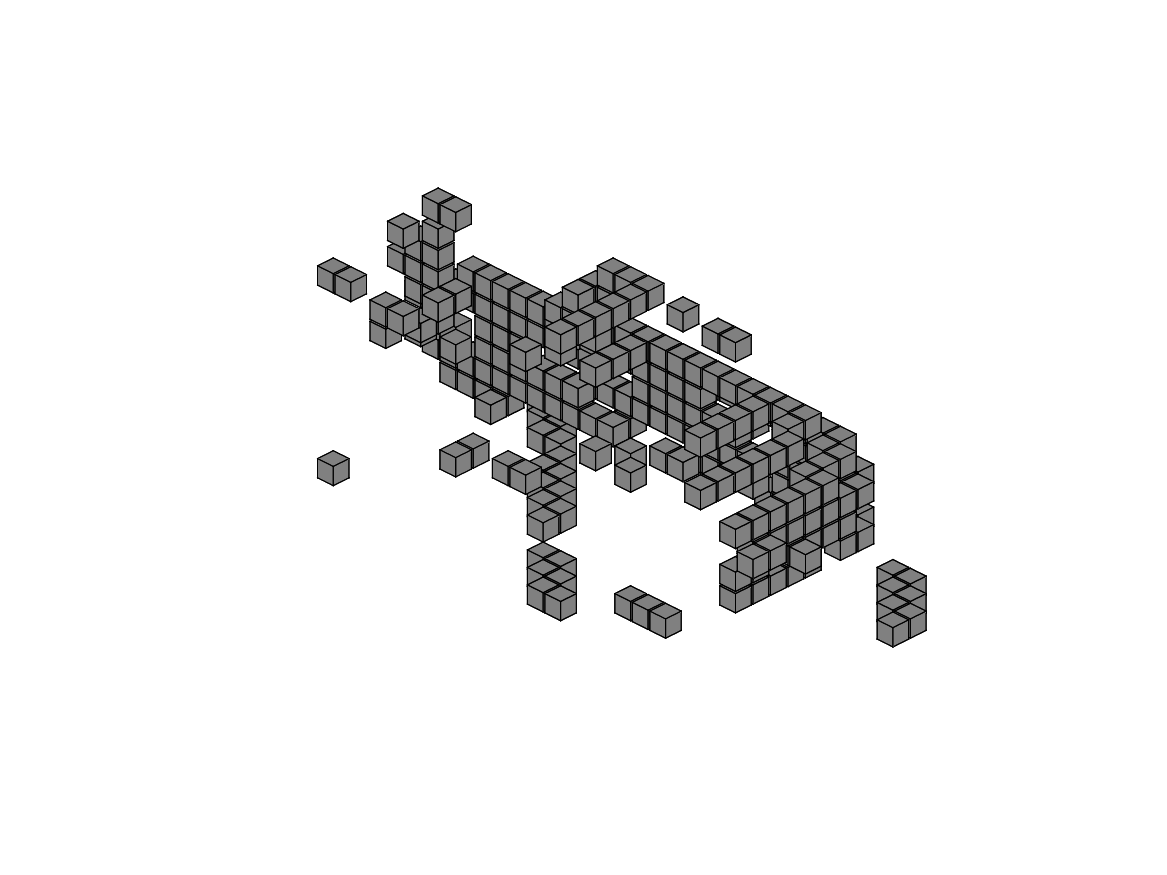
\includegraphics[height=1.5cm,trim={3cm 2cm 3cm 2cm},clip]{images/0_input_45}
        };
        
        \node[transparent] at (2.3, 0) {\footnotesize Encoder};
        \draw[transparent,-] ($(input.north east) + (0.25,0)$) -- (3.25,0.5);
        \draw[transparent,-] ($(input.south east) + (0.25,0)$) -- (3.25,-0.5);
        \draw[transparent,-] ($(input.south east) + (0.25,0)$) -- ($(input.north east) + (0.25,0)$);
        \draw[transparent,-] (3.25,-0.5) -- (3.25,0.5);
        
        \node (z) at (3.5, 0) {\footnotesize $z$};
        
        \node[rectangle,draw=black] (output) at (7, 0) {
          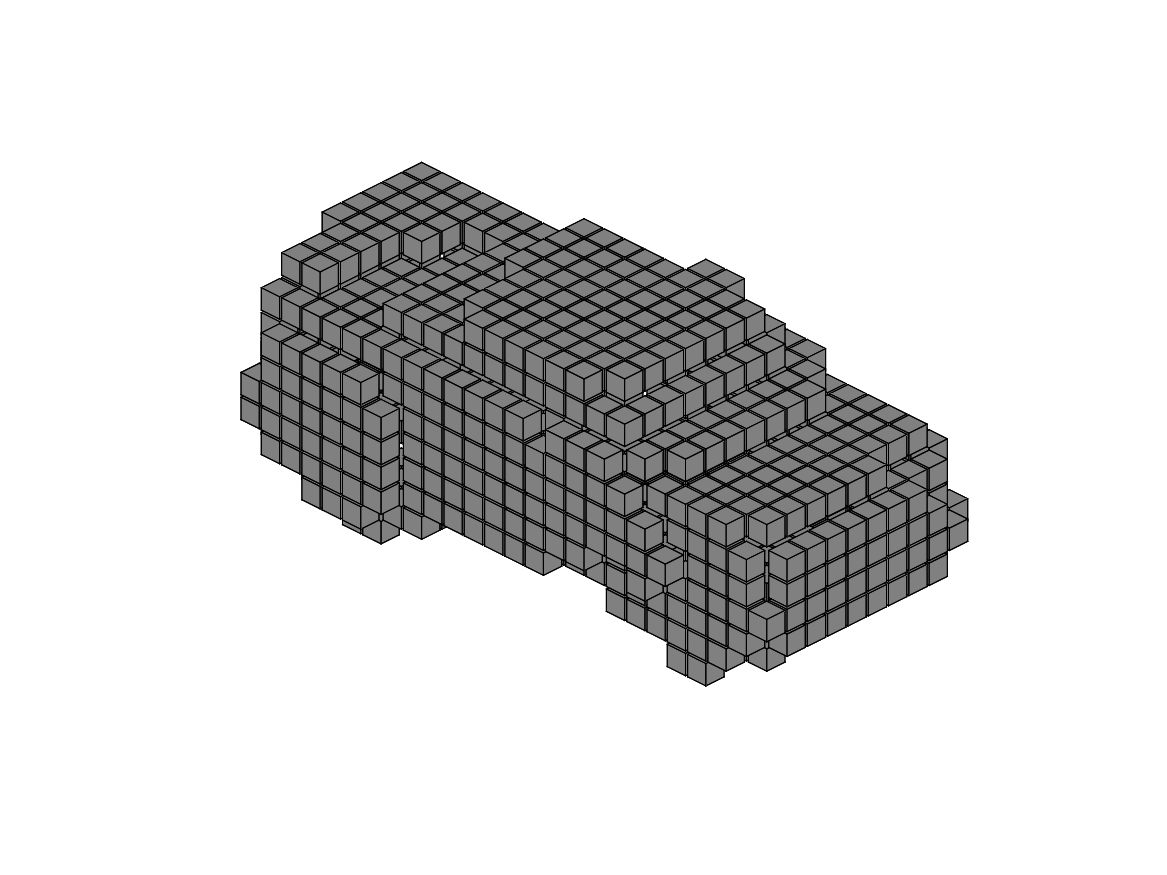
\includegraphics[height=1.5cm,trim={3cm 2cm 3cm 2cm},clip]{images/0_prediction_45}
        };
        
        \node at (4.7, 0) {\footnotesize Decoder};
        \draw[-] ($(output.north west) - (0.25,0)$) -- (3.75,0.5);
        \draw[-] ($(output.south west) - (0.25,0)$) -- (3.75,-0.5);
        \draw[-] ($(output.south west) - (0.25,0)$) -- ($(output.north west) - (0.25,0)$);
        \draw[-] (3.75,-0.5) -- (3.75,0.5);
        
        \node (ry) at (8.5, 0) {\footnotesize $\tilde{y}$};
        
        \node[transparent,color=RWTHdarkorange] at (-0.2,1.4) {\footnotesize Deterministic $z(x)$};

        \node[transparent,rectangle,dashed,draw=RWTHdarkorange,minimum width=5.2cm,minimum height=3cm] at (0.7, 0.25) {};
        
        \node[color=RWTHgreen] at (6,1.4) {\footnotesize Generative Model $p(y|z) p(z)$};

        \node[rectangle,dashed,draw=RWTHgreen,minimum width=5.5cm,minimum height=3cm] at (6.1, 0.25) {};
        
        \node[] (L) at (3.5, -2) {\footnotesize Maximum Likelihood};
            
        \draw[-] (ry) -- ($(ry) - (0,2)$);
        \draw[-] ($(ry) - (0,2)$) -- (L);
        \draw[-] (y) -- ($(y) - (0,2)$);
        \draw[-] ($(y) - (0,2)$) -- (L);
      \end{tikzpicture}
      }
    \end{center}
  \end{frame}
  
  \begin{frame}
    {\large Shape Inference}
    
    Minimize the negative log-likelihood of observation $x$ over the latent space:
    \begin{align}
      &\argmin_z - \ln p(y = x, z)\notag\\
      =&\argmin_z - \sum_i \ln p(y_i = x_i | z) - \ln p(z)\notag
    \end{align}
    \vspace*{-1cm}
    
    \begin{center}
      {\setbeamercovered{transparent}
      \begin{tikzpicture}
        \node[] (y) at (-1.5, 0) {\footnotesize $x$};
            
        \node[rectangle,draw=black] (input) at (0, 0) {
          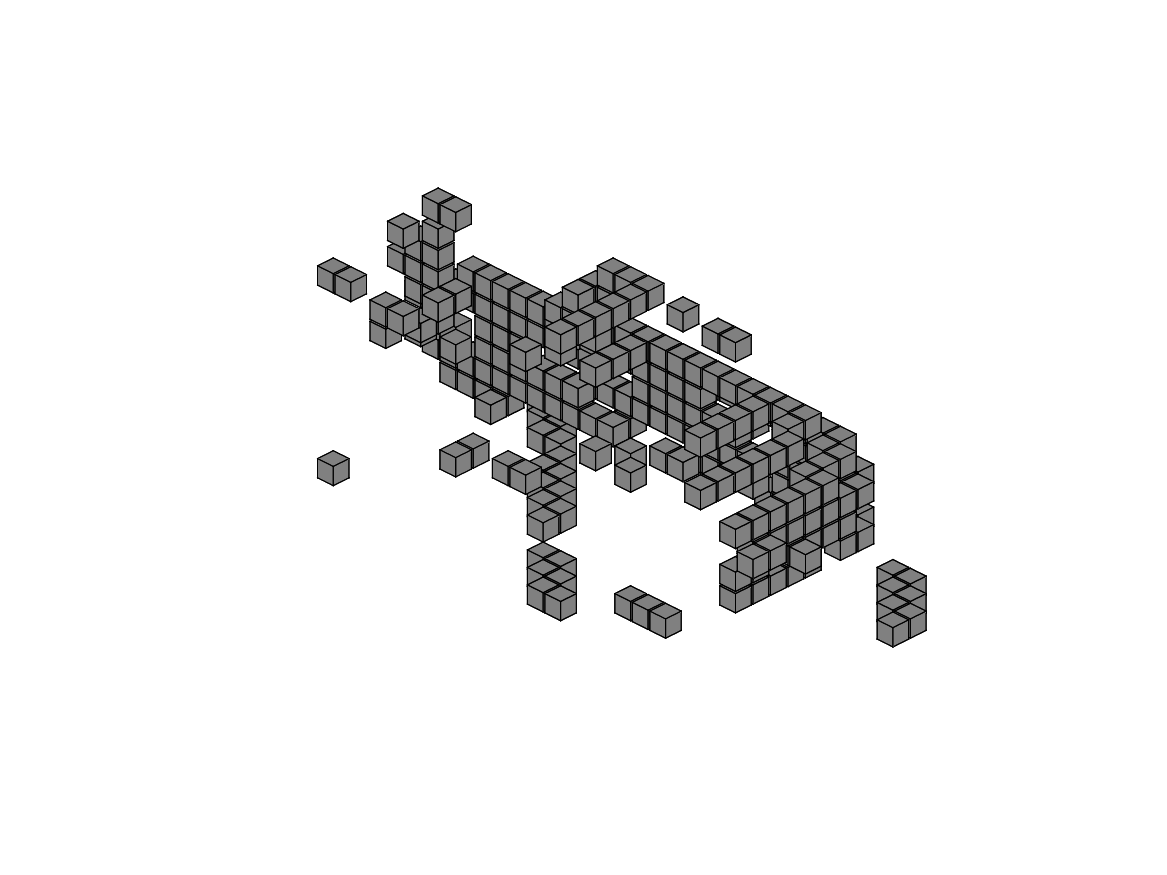
\includegraphics[height=1.5cm,trim={3cm 2cm 3cm 2cm},clip]{images/0_input_45}
        };
        
        \node[transparent] at (2.3, 0) {\footnotesize Encoder};
        \draw[transparent,-] ($(input.north east) + (0.25,0)$) -- (3.25,0.5);
        \draw[transparent,-] ($(input.south east) + (0.25,0)$) -- (3.25,-0.5);
        \draw[transparent,-] ($(input.south east) + (0.25,0)$) -- ($(input.north east) + (0.25,0)$);
        \draw[transparent,-] (3.25,-0.5) -- (3.25,0.5);
        
        \node (z) at (3.5, 0) {\footnotesize $z$};
        
        \node[rectangle,draw=black] (output) at (7, 0) {
          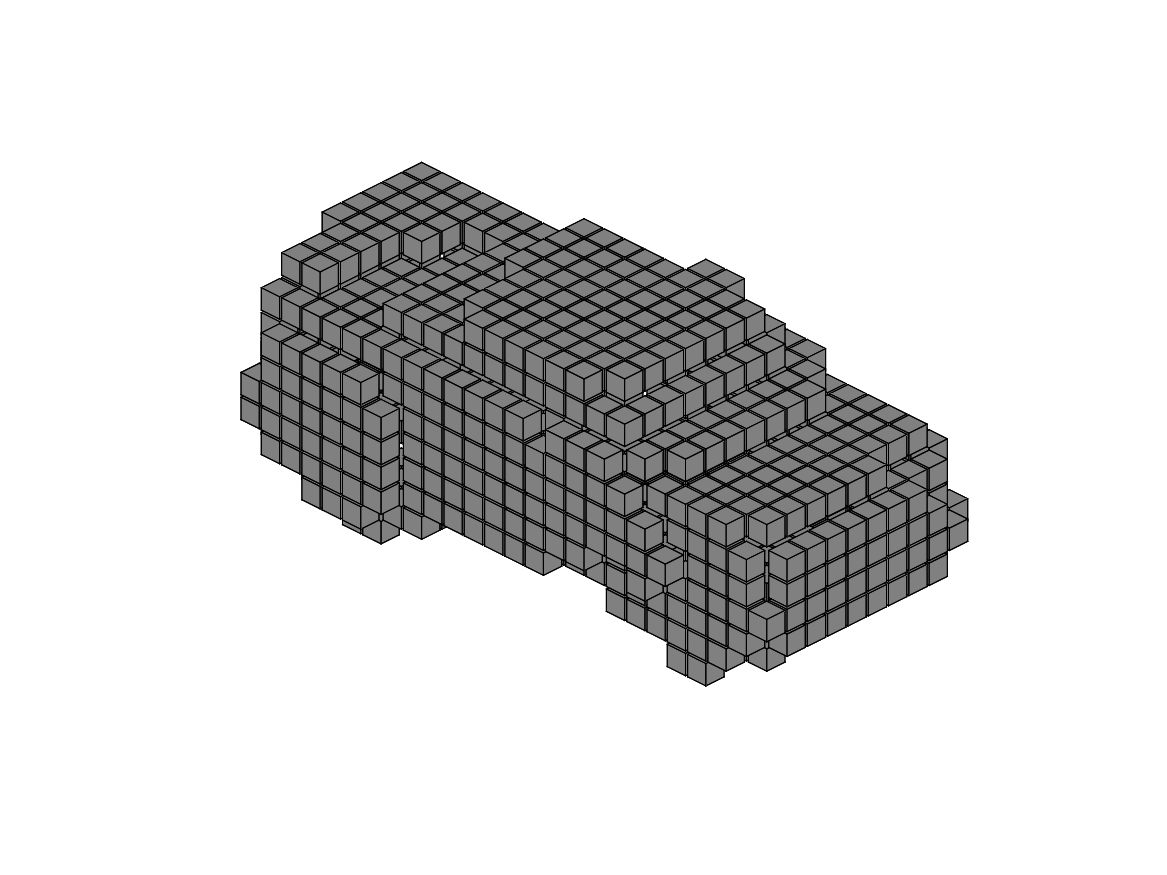
\includegraphics[height=1.5cm,trim={3cm 2cm 3cm 2cm},clip]{images/0_prediction_45}
        };
        
        \node at (4.7, 0) {\footnotesize Decoder};
        \draw[-] ($(output.north west) - (0.25,0)$) -- (3.75,0.5);
        \draw[-] ($(output.south west) - (0.25,0)$) -- (3.75,-0.5);
        \draw[-] ($(output.south west) - (0.25,0)$) -- ($(output.north west) - (0.25,0)$);
        \draw[-] (3.75,-0.5) -- (3.75,0.5);
        
        \node (ry) at (8.5, 0) {\footnotesize $\tilde{y}$};
        
        \node[transparent,color=RWTHdarkorange] at (-0.2,1.4) {\footnotesize Deterministic $z(x)$};
        \node[transparent,rectangle,dashed,draw=RWTHdarkorange,minimum width=5.2cm,minimum height=3cm] at (0.7, 0.25) {};
        
        \node[color=RWTHgreen] at (6,1.4) {\footnotesize Generative Model $p(y|z) p(z)$};
        \node[rectangle,dashed,draw=RWTHgreen,minimum width=5.5cm,minimum height=3cm] at (6.1, 0.25) {};
        
        \node[] (L) at (3.5, -2) {\footnotesize Maximum Likelihood};
            
        \draw[-] (ry) -- ($(ry) - (0,2)$);
        \draw[-] ($(ry) - (0,2)$) -- (L);
        \draw[-] (y) -- ($(y) - (0,2)$);
        \draw[-] ($(y) - (0,2)$) -- (L);
        \fill[white,path fading=north] (-2,2) rectangle (10,-3);
      \end{tikzpicture}
      }
    \end{center}
  \end{frame}
  
  \begin{frame}
    {\large Shape Inference}
    
    Minimize the negative log-likelihood of observation $x$ over the latent space:
    \begin{align}
      &\argmin_z - \ln p(y = x, z)\notag\\
      =&\argmin_z {\color{RWTHred} \sum_i \mathcal{L}_{\text{BCE}}(\tilde{y}_i, x_i)} - \ln p(z)\notag
    \end{align}
    \vspace*{-1cm}
    
    \begin{center}
      {\setbeamercovered{transparent}
      \begin{tikzpicture}
        \node[] (y) at (-1.5, 0) {\footnotesize $x$};
            
        \node[rectangle,draw=black] (input) at (0, 0) {
          \includegraphics[height=1.5cm,trim={3cm 2cm 3cm 2cm},clip]{images/0_input_45}
        };
        
        \node[transparent] at (2.3, 0) {\footnotesize Encoder};
        \draw[transparent,-] ($(input.north east) + (0.25,0)$) -- (3.25,0.5);
        \draw[transparent,-] ($(input.south east) + (0.25,0)$) -- (3.25,-0.5);
        \draw[transparent,-] ($(input.south east) + (0.25,0)$) -- ($(input.north east) + (0.25,0)$);
        \draw[transparent,-] (3.25,-0.5) -- (3.25,0.5);
        
        \node (z) at (3.5, 0) {\footnotesize $z$};
        
        \node[rectangle,draw=black] (output) at (7, 0) {
          \includegraphics[height=1.5cm,trim={3cm 2cm 3cm 2cm},clip]{images/0_prediction_45}
        };
        
        \node at (4.7, 0) {\footnotesize Decoder};
        \draw[-] ($(output.north west) - (0.25,0)$) -- (3.75,0.5);
        \draw[-] ($(output.south west) - (0.25,0)$) -- (3.75,-0.5);
        \draw[-] ($(output.south west) - (0.25,0)$) -- ($(output.north west) - (0.25,0)$);
        \draw[-] (3.75,-0.5) -- (3.75,0.5);
        
        \node (ry) at (8.5, 0) {\footnotesize $\tilde{y}$};
        
        \node[transparent,color=RWTHdarkorange] at (-0.2,1.4) {\footnotesize Deterministic $z(x)$};
        \node[transparent,rectangle,dashed,draw=RWTHdarkorange,minimum width=5.2cm,minimum height=3cm] at (0.7, 0.25) {};
        
        \node[color=RWTHgreen] at (6,1.4) {\footnotesize Generative Model $p(y|z) p(z)$};
        \node[rectangle,dashed,draw=RWTHgreen,minimum width=5.5cm,minimum height=3cm] at (6.1, 0.25) {};
        
        \node[] (L) at (3.5, -2) {\footnotesize Maximum Likelihood};
            
        \draw[-] (ry) -- ($(ry) - (0,2)$);
        \draw[-] ($(ry) - (0,2)$) -- (L);
        \draw[-] (y) -- ($(y) - (0,2)$);
        \draw[-] ($(y) - (0,2)$) -- (L);
        \fill[white,path fading=north] (-2,2) rectangle (10,-3);
      \end{tikzpicture}
      }
    \end{center}
  \end{frame}
  
  \begin{frame}
    {\large Shape Inference}
    
    Minimize the negative log-likelihood of observation $x$ over the latent space:
    \begin{align}
      &\argmin_z - \ln p(y = x, z)\notag\\
      =&\argmin_z \sum_i \mathcal{L}_{\text{BCE}}(\tilde{y}_i, x_i) {\color{RWTHred}+ \text{const} + \frac{1}{2} \|z\|_2^2}\notag
    \end{align}
    \vspace*{-1.2cm}
    
    \begin{center}
      {\setbeamercovered{transparent}
      \begin{tikzpicture}
        \node[] (y) at (-1.5, 0) {\footnotesize $x$};
            
        \node[rectangle,draw=black] (input) at (0, 0) {
          \includegraphics[height=1.5cm,trim={3cm 2cm 3cm 2cm},clip]{images/0_input_45}
        };
        
        \node[transparent] at (2.3, 0) {\footnotesize Encoder};
        \draw[transparent,-] ($(input.north east) + (0.25,0)$) -- (3.25,0.5);
        \draw[transparent,-] ($(input.south east) + (0.25,0)$) -- (3.25,-0.5);
        \draw[transparent,-] ($(input.south east) + (0.25,0)$) -- ($(input.north east) + (0.25,0)$);
        \draw[transparent,-] (3.25,-0.5) -- (3.25,0.5);
        
        \node (z) at (3.5, 0) {\footnotesize $z$};
        
        \node[rectangle,draw=black] (output) at (7, 0) {
          \includegraphics[height=1.5cm,trim={3cm 2cm 3cm 2cm},clip]{images/0_prediction_45}
        };
        
        \node at (4.7, 0) {\footnotesize Decoder};
        \draw[-] ($(output.north west) - (0.25,0)$) -- (3.75,0.5);
        \draw[-] ($(output.south west) - (0.25,0)$) -- (3.75,-0.5);
        \draw[-] ($(output.south west) - (0.25,0)$) -- ($(output.north west) - (0.25,0)$);
        \draw[-] (3.75,-0.5) -- (3.75,0.5);
        
        \node (ry) at (8.5, 0) {\footnotesize $\tilde{y}$};
        
        \node[transparent,color=RWTHdarkorange] at (-0.2,1.4) {\footnotesize Deterministic $z(x)$};
        \node[transparent,rectangle,dashed,draw=RWTHdarkorange,minimum width=5.2cm,minimum height=3cm] at (0.7, 0.25) {};
        
        \node[color=RWTHgreen] at (6,1.4) {\footnotesize Generative Model $p(y|z) p(z)$};
        \node[rectangle,dashed,draw=RWTHgreen,minimum width=5.5cm,minimum height=3cm] at (6.1, 0.25) {};
        
        \node[] (L) at (3.5, -2) {\footnotesize Maximum Likelihood};
            
        \draw[-] (ry) -- ($(ry) - (0,2)$);
        \draw[-] ($(ry) - (0,2)$) -- (L);
        \draw[-] (y) -- ($(y) - (0,2)$);
        \draw[-] ($(y) - (0,2)$) -- (L);
        \fill[white,path fading=north] (-2,2) rectangle (10,-3);
      \end{tikzpicture}
      }
    \end{center}
  \end{frame}
  
  \begin{frame}
    {\large Shape Inference}
    
    What observations do we have?
    \begin{itemize}
      \item Occupied voxels $x_i = 1$ (from observed points);
      \item[]
      \item[]
    \end{itemize}
    
    \begin{center}
      %\vspace{0.5cm}
      \begin{tikzpicture}
        
        \node[transparent,rectangle,draw=black,fill=white] at (-2.1, 0) {
          \includegraphics[height=2.4cm,trim={3cm 2cm 3cm 2cm},clip]{images/0_space_45}
        };
        \node[transparent] at (-2.1, -2) {\Scriptsize\begin{tabular}{c}Free Space\\Voxels $x_i = 0$\end{tabular}};
        
        \node[rectangle,draw=black,fill=white] at (1.4, 0) {
          \includegraphics[height=2.4cm,trim={3cm 2cm 3cm 2cm},clip]{images/0_input_45}
        };
        \node at (1.4, -2) {\Scriptsize\begin{tabular}{c}Occupied\\Voxels $x_i = 1$\end{tabular}};
        
        \node[transparent,rectangle,draw=RWTHred,fill=white] at (4.9, 0) {
          \includegraphics[height=2.4cm,trim={3cm 2cm 3cm 2cm},clip]{images/0_baseline_prediction_45}
        };
        \node[transparent] at (4.9, -2) {\Scriptsize\color{RWTHred} Unknown Shape $y^*$};
      \end{tikzpicture}
      \vspace*{-0.5cm}
    \end{center}
  \end{frame}
  
  \begin{frame}
    {\large Shape Inference}
    
    What observations do we have?
    \begin{itemize}
      \item Occupied voxels $x_i = 1$ (from observed points);
      \item unoccupied voxels $x_i = 0$ (from free space);
      \item[]
    \end{itemize}
    
    \begin{center}
      %\vspace{0.5cm}
      \begin{tikzpicture}
        
        \node[rectangle,draw=black,fill=white] at (-2.1, 0) {
          \includegraphics[height=2.4cm,trim={3cm 2cm 3cm 2cm},clip]{images/0_space_45}
        };
        \node at (-2.1, -2) {\Scriptsize\begin{tabular}{c}Free Space\\Voxels $x_i = 0$\end{tabular}};
        
        \node[rectangle,draw=black,fill=white] at (1.4, 0) {
          \includegraphics[height=2.4cm,trim={3cm 2cm 3cm 2cm},clip]{images/0_input_45}
        };
        \node at (1.4, -2) {\Scriptsize\begin{tabular}{c}Occupied\\Voxels $x_i = 1$\end{tabular}};
        
        \node[transparent,rectangle,draw=RWTHred,fill=white] at (4.9, 0) {
          \includegraphics[height=2.4cm,trim={3cm 2cm 3cm 2cm},clip]{images/0_baseline_prediction_45}
        };
        \node[transparent] at (4.9, -2) {\Scriptsize\color{RWTHred} Unknown Shape $y^*$};
      \end{tikzpicture}
      \vspace*{-0.5cm}
    \end{center}
  \end{frame}
  
  \begin{frame}
    {\large Shape Inference}
    
    What observations do we have?
    \begin{itemize}
      \item Occupied voxels $x_i = 1$ (from observed points);
      \item unoccupied voxels $x_i = 0$ (from free space);
      \item and {\color{RWTHred}unknown voxels ``$x_i = \uk$''}.
    \end{itemize}
    
    \begin{center}
      %\vspace{0.5cm}
      \begin{tikzpicture}
        
        \node[rectangle,draw=black,fill=white] at (-2.1, 0) {
          \includegraphics[height=2.4cm,trim={3cm 2cm 3cm 2cm},clip]{images/0_space_45}
        };
        \node at (-2.1, -2) {\Scriptsize\begin{tabular}{c}Free Space\\Voxels $x_i = 0$\end{tabular}};
        
        \node[rectangle,draw=black,fill=white] at (1.4, 0) {
          \includegraphics[height=2.4cm,trim={3cm 2cm 3cm 2cm},clip]{images/0_input_45}
        };
        \node at (1.4, -2) {\Scriptsize\begin{tabular}{c}Occupied\\Voxels $x_i = 1$\end{tabular}};
        
        \node[rectangle,draw=RWTHred,fill=white] at (4.9, 0) {
          \includegraphics[height=2.4cm,trim={3cm 2cm 3cm 2cm},clip]{images/0_baseline_prediction_45}
        };
        \node at (4.9, -2) {\Scriptsize\color{RWTHred} Unknown Shape $y^*$};
      \end{tikzpicture}
      \vspace*{-0.5cm}
    \end{center}
  \end{frame}
  
  \begin{frame}
    {\large Shape Inference}
    
    Minimize the negative log-likelihood of observation $x$ over the latent space:
    \begin{align}
      &\argmin_z - \ln p(y = x, z)\notag\\
      =&\argmin_z \sum_{\color{RWTHred} x_i \neq \uk} \mathcal{L}_{\text{BCE}}(\tilde{y}_i, x_i) + \text{const} + \frac{1}{2} \|z\|_2^2\notag
    \end{align}
    
    \begin{center}
      \vspace{-0.5cm}
      \begin{tikzpicture}
        
        \node[rectangle,draw=black,fill=white] at (-2.1, 0) {
          \includegraphics[height=2.4cm,trim={3cm 2cm 3cm 2cm},clip]{images/0_space_45}
        };
        \node at (-2.1, -2) {\Scriptsize\begin{tabular}{c}Free Space\\Voxels $x_i = 0$\end{tabular}};
        
        \node[rectangle,draw=black,fill=white] at (1.4, 0) {
          \includegraphics[height=2.4cm,trim={3cm 2cm 3cm 2cm},clip]{images/0_input_45}
        };
        \node at (1.4, -2) {\Scriptsize\begin{tabular}{c}Occupied\\Voxels $x_i = 1$\end{tabular}};
        
        \node[rectangle,draw=RWTHred,fill=white] at (4.9, 0) {
          \includegraphics[height=2.4cm,trim={3cm 2cm 3cm 2cm},clip]{images/0_baseline_prediction_45}
        };
        \node at (4.9, -2) {\Scriptsize\color{RWTHred} Unknown Shape $y^*$};
        \fill[white,path fading=north] (-4,2) rectangle (7,-2.5);
      \end{tikzpicture}
      \vspace*{-0.5cm}
    \end{center}
  \end{frame}
  
  \begin{frame}[t]
    {\large Shape Inference}
    
    Minimize the negative log-likelihood of observation $x$ over the latent space:
    \begin{center}
      {\setbeamercovered{transparent}
      \begin{tikzpicture}
        \node[] (y) at (-1.5, 0) {\footnotesize $x$};
            
        \node[rectangle,draw=black] (input) at (0, 0) {
          \includegraphics[height=1.5cm,trim={3cm 2cm 3cm 2cm},clip]{images/0_input_45}
        };
        
        \node[transparent] at (2.3, 0) {\footnotesize Encoder};
        \draw[transparent,-] ($(input.north east) + (0.25,0)$) -- (3.25,0.5);
        \draw[transparent,-] ($(input.south east) + (0.25,0)$) -- (3.25,-0.5);
        \draw[transparent,-] ($(input.south east) + (0.25,0)$) -- ($(input.north east) + (0.25,0)$);
        \draw[transparent,-] (3.25,-0.5) -- (3.25,0.5);
        
        \node (z) at (3.5, 0) {\footnotesize $z$};
        
        \node[rectangle,draw=black] (output) at (7, 0) {
          \includegraphics[height=1.5cm,trim={3cm 2cm 3cm 2cm},clip]{images/0_prediction_45}
        };
        
        \node at (4.7, 0) {\footnotesize Decoder};
        \draw[-] ($(output.north west) - (0.25,0)$) -- (3.75,0.5);
        \draw[-] ($(output.south west) - (0.25,0)$) -- (3.75,-0.5);
        \draw[-] ($(output.south west) - (0.25,0)$) -- ($(output.north west) - (0.25,0)$);
        \draw[-] (3.75,-0.5) -- (3.75,0.5);
        
        \node (ry) at (8.5, 0) {\footnotesize $\tilde{y}$};
        
        \node[transparent,color=RWTHdarkorange] at (-0.2,1.4) {\footnotesize Deterministic $z(x)$};
        \node[transparent,rectangle,dashed,draw=RWTHdarkorange,minimum width=5.2cm,minimum height=3cm] at (0.7, 0.25) {};
        
        \node[color=RWTHgreen] at (6,1.4) {\footnotesize Generative Model $p(y|z) p(z)$};
        \node[rectangle,dashed,draw=RWTHgreen,minimum width=5.5cm,minimum height=3cm] at (6.1, 0.25) {};
        
        \node[] (L) at (3.5, -2) {\footnotesize Maximum Likelihood};
            
        \draw[-] (ry) -- ($(ry) - (0,2)$);
        \draw[-] ($(ry) - (0,2)$) -- (L);
        \draw[-] (y) -- ($(y) - (0,2)$);
        \draw[-] ($(y) - (0,2)$) -- (L);
      \end{tikzpicture}
      }
    \end{center}
  \end{frame}
  
  \begin{frame}[t]
    {\large Shape Inference}
    
    \textbf{Learn} to minimize the negative log-likelihood of observation $x$
    over the latent space:
    
    \begin{center}
      {\setbeamercovered{transparent}
      \begin{tikzpicture}
        \node[] (y) at (-1.5, 0) {\footnotesize $x$};
            
        \node[rectangle,draw=black] (input) at (0, 0) {
          \includegraphics[height=1.5cm,trim={3cm 2cm 3cm 2cm},clip]{images/0_input_45}
        };
        
        \node[] at (2.3, 0) {\footnotesize Encoder};
        \draw[-] ($(input.north east) + (0.25,0)$) -- (3.25,0.5);
        \draw[-] ($(input.south east) + (0.25,0)$) -- (3.25,-0.5);
        \draw[-] ($(input.south east) + (0.25,0)$) -- ($(input.north east) + (0.25,0)$);
        \draw[-] (3.25,-0.5) -- (3.25,0.5);
        
        \node (z) at (3.5, 0) {\footnotesize $z$};
        
        \node[rectangle,draw=black] (output) at (7, 0) {
          \includegraphics[height=1.5cm,trim={3cm 2cm 3cm 2cm},clip]{images/0_prediction_45}
        };
        
        \node at (4.7, 0) {\footnotesize Decoder};
        \draw[-] ($(output.north west) - (0.25,0)$) -- (3.75,0.5);
        \draw[-] ($(output.south west) - (0.25,0)$) -- (3.75,-0.5);
        \draw[-] ($(output.south west) - (0.25,0)$) -- ($(output.north west) - (0.25,0)$);
        \draw[-] (3.75,-0.5) -- (3.75,0.5);
        
        \node (ry) at (8.5, 0) {\footnotesize $\tilde{y}$};
        
        \node[color=RWTHdarkorange] at (-0.2,1.4) {\footnotesize Deterministic $z(x)$};
        \node[rectangle,dashed,draw=RWTHdarkorange,minimum width=5.2cm,minimum height=3cm] at (0.7, 0.25) {};
        
        \node[color=RWTHgreen] at (6,1.4) {\footnotesize Generative Model $p(y|z) p(z)$};
        \node[rectangle,dashed,draw=RWTHgreen,minimum width=5.5cm,minimum height=3cm] at (6.1, 0.25) {};
        
        \node[] (L) at (3.5, -2) {\footnotesize \begin{tabular}{c}Unsupervised\\Maximum Likelihood Loss\end{tabular}};
            
        \draw[-] (ry) -- ($(ry) - (0,2)$);
        \draw[-] ($(ry) - (0,2)$) -- (L);
        \draw[-] (y) -- ($(y) - (0,2)$);
        \draw[-] ($(y) - (0,2)$) -- (L);
      \end{tikzpicture}
      }
    \end{center}
  \end{frame}
  
  \begin{frame}
    {\large Shape Inference}
    
    \textbf{Learn} to minimize the negative log-likelihood of observation $x$
    over the latent space:
    \begin{align}
      x \mapsto \tilde{z}(x) \approx \argmin_z - \sum_{ x_i \neq \uk} \ln p(y_i = x_i | z) - \ln p(z)\notag
    \end{align}
    
    \begin{center}
      {\setbeamercovered{transparent}
      \begin{tikzpicture}
        \node[] (y) at (-1.5, 0) {\footnotesize $x$};
            
        \node[rectangle,draw=black] (input) at (0, 0) {
          \includegraphics[height=1.5cm,trim={3cm 2cm 3cm 2cm},clip]{images/0_input_45}
        };
        
        \node[] at (2.3, 0) {\footnotesize Encoder};
        \draw[-] ($(input.north east) + (0.25,0)$) -- (3.25,0.5);
        \draw[-] ($(input.south east) + (0.25,0)$) -- (3.25,-0.5);
        \draw[-] ($(input.south east) + (0.25,0)$) -- ($(input.north east) + (0.25,0)$);
        \draw[-] (3.25,-0.5) -- (3.25,0.5);
        
        \node (z) at (3.5, 0) {\footnotesize $z$};
        
        \node[rectangle,draw=black] (output) at (7, 0) {
          \includegraphics[height=1.5cm,trim={3cm 2cm 3cm 2cm},clip]{images/0_prediction_45}
        };
        
        \node at (4.7, 0) {\footnotesize Decoder};
        \draw[-] ($(output.north west) - (0.25,0)$) -- (3.75,0.5);
        \draw[-] ($(output.south west) - (0.25,0)$) -- (3.75,-0.5);
        \draw[-] ($(output.south west) - (0.25,0)$) -- ($(output.north west) - (0.25,0)$);
        \draw[-] (3.75,-0.5) -- (3.75,0.5);
        
        \node (ry) at (8.5, 0) {\footnotesize $\tilde{y}$};
        
        \node[color=RWTHdarkorange] at (-0.2,1.4) {\footnotesize Deterministic $z(x)$};
        \node[rectangle,dashed,draw=RWTHdarkorange,minimum width=5.2cm,minimum height=3cm] at (0.7, 0.25) {};
        
        \node[color=RWTHgreen] at (6,1.4) {\footnotesize Generative Model $p(y|z) p(z)$};
        \node[rectangle,dashed,draw=RWTHgreen,minimum width=5.5cm,minimum height=3cm] at (6.1, 0.25) {};
        
        \node[] (L) at (3.5, -2) {\footnotesize \begin{tabular}{c}Unsupervised\\Maximum Likelihood Loss\end{tabular}};
            
        \draw[-] (ry) -- ($(ry) - (0,2)$);
        \draw[-] ($(ry) - (0,2)$) -- (L);
        \draw[-] (y) -- ($(y) - (0,2)$);
        \draw[-] ($(y) - (0,2)$) -- (L);
        \fill[white,path fading=north] (-2,2) rectangle (10,-3);
      \end{tikzpicture}
      \vspace{-2cm}
      }
    \end{center}
  \end{frame}
  
  \begin{frame}
    {\large Shape Inference}
    
    \textbf{Learn} to minimize the negative log-likelihood of observation $x$
    over the latent space:
    \begin{align}
      \mathcal{L}(\tilde{y}, x) = - \sum_{x_i \neq \uk} \ln p(\tilde{y}_i = x_i | z) - \ln p(z)\notag
    \end{align}
    
    \begin{center}
      {\setbeamercovered{transparent}
      \begin{tikzpicture}
        \node[] (y) at (-1.5, 0) {\footnotesize $x$};
            
        \node[rectangle,draw=black] (input) at (0, 0) {
          \includegraphics[height=1.5cm,trim={3cm 2cm 3cm 2cm},clip]{images/0_input_45}
        };
        
        \node[] at (2.3, 0) {\footnotesize Encoder};
        \draw[-] ($(input.north east) + (0.25,0)$) -- (3.25,0.5);
        \draw[-] ($(input.south east) + (0.25,0)$) -- (3.25,-0.5);
        \draw[-] ($(input.south east) + (0.25,0)$) -- ($(input.north east) + (0.25,0)$);
        \draw[-] (3.25,-0.5) -- (3.25,0.5);
        
        \node (z) at (3.5, 0) {\footnotesize $z$};
        
        \node[rectangle,draw=black] (output) at (7, 0) {
          \includegraphics[height=1.5cm,trim={3cm 2cm 3cm 2cm},clip]{images/0_prediction_45}
        };
        
        \node at (4.7, 0) {\footnotesize Decoder};
        \draw[-] ($(output.north west) - (0.25,0)$) -- (3.75,0.5);
        \draw[-] ($(output.south west) - (0.25,0)$) -- (3.75,-0.5);
        \draw[-] ($(output.south west) - (0.25,0)$) -- ($(output.north west) - (0.25,0)$);
        \draw[-] (3.75,-0.5) -- (3.75,0.5);
        
        \node (ry) at (8.5, 0) {\footnotesize $\tilde{y}$};
        
        \node[color=RWTHdarkorange] at (-0.2,1.4) {\footnotesize Deterministic $z(x)$};
        \node[rectangle,dashed,draw=RWTHdarkorange,minimum width=5.2cm,minimum height=3cm] at (0.7, 0.25) {};
        
        \node[color=RWTHgreen] at (6,1.4) {\footnotesize Generative Model $p(y|z) p(z)$};
        \node[rectangle,dashed,draw=RWTHgreen,minimum width=5.5cm,minimum height=3cm] at (6.1, 0.25) {};
        
        \node[] (L) at (3.5, -2) {\footnotesize $\mathcal{L}(\tilde{y}, x)$};
            
        \draw[-] (ry) -- ($(ry) - (0,2)$);
        \draw[-] ($(ry) - (0,2)$) -- (L);
        \draw[-] (y) -- ($(y) - (0,2)$);
        \draw[-] ($(y) - (0,2)$) -- (L);
        \fill[white,path fading=north] (-2,2) rectangle (10,-3);
      \end{tikzpicture}
      \vspace{-2cm}
      }
    \end{center}
  \end{frame}
  
  \begin{frame}
    {\large Shape Inference}
    
    \textbf{Learn} to minimize the negative log-likelihood of observation $x$
    over the latent space:
    \begin{align}
      \mathcal{L}(\tilde{y}, x) = {\color{RWTHred} \sum_{x_i \neq \uk} \mathcal{L}_{\text{BCE}}(\tilde{y}_i, x_i)} - \ln p(z)\hphantom{(x)\|^2}\notag
    \end{align}
    
    \begin{center}
      {\setbeamercovered{transparent}
      \begin{tikzpicture}
        \node[] (y) at (-1.5, 0) {\footnotesize $x$};

            
        \node[rectangle,draw=black] (input) at (0, 0) {
          \includegraphics[height=1.5cm,trim={3cm 2cm 3cm 2cm},clip]{images/0_input_45}
        };
        
        \node[] at (2.3, 0) {\footnotesize Encoder};
        \draw[-] ($(input.north east) + (0.25,0)$) -- (3.25,0.5);
        \draw[-] ($(input.south east) + (0.25,0)$) -- (3.25,-0.5);
        \draw[-] ($(input.south east) + (0.25,0)$) -- ($(input.north east) + (0.25,0)$);
        \draw[-] (3.25,-0.5) -- (3.25,0.5);
        
        \node (z) at (3.5, 0) {\footnotesize $z$};
        
        \node[rectangle,draw=black] (output) at (7, 0) {
          \includegraphics[height=1.5cm,trim={3cm 2cm 3cm 2cm},clip]{images/0_prediction_45}
        };
        
        \node at (4.7, 0) {\footnotesize Decoder};
        \draw[-] ($(output.north west) - (0.25,0)$) -- (3.75,0.5);
        \draw[-] ($(output.south west) - (0.25,0)$) -- (3.75,-0.5);
        \draw[-] ($(output.south west) - (0.25,0)$) -- ($(output.north west) - (0.25,0)$);
        \draw[-] (3.75,-0.5) -- (3.75,0.5);
        
        \node (ry) at (8.5, 0) {\footnotesize $\tilde{y}$};
        
        \node[color=RWTHdarkorange] at (-0.2,1.4) {\footnotesize Deterministic $z(x)$};
        \node[rectangle,dashed,draw=RWTHdarkorange,minimum width=5.2cm,minimum height=3cm] at (0.7, 0.25) {};
        
        \node[color=RWTHgreen] at (6,1.4) {\footnotesize Generative Model $p(y|z) p(z)$};
        \node[rectangle,dashed,draw=RWTHgreen,minimum width=5.5cm,minimum height=3cm] at (6.1, 0.25) {};
        
        \node[] (L) at (3.5, -2) {\footnotesize $\mathcal{L}(\tilde{y}, x)$};
            
        \draw[-] (ry) -- ($(ry) - (0,2)$);
        \draw[-] ($(ry) - (0,2)$) -- (L);
        \draw[-] (y) -- ($(y) - (0,2)$);
        \draw[-] ($(y) - (0,2)$) -- (L);
        \fill[white,path fading=north] (-2,2) rectangle (10,-3);
      \end{tikzpicture}
      \vspace{-2cm}
      }
    \end{center}
  \end{frame}
  
  \begin{frame}
    {\large Shape Inference}
    
    \textbf{Learn} to minimize the negative log-likelihood of observation $x$
    over the latent space:
    \begin{align}
      \mathcal{L}(\tilde{y}, x) = \sum_{x_i \neq \uk} \mathcal{L}_{\text{BCE}}(\tilde{y}_i, x_i) {+ \color{RWTHred} \text{const} + \frac{1}{2}\|z(x)\|_2^2}\notag
    \end{align}
    
    \begin{center}
      {\setbeamercovered{transparent}
      \begin{tikzpicture}
        \node[] (y) at (-1.5, 0) {\footnotesize $x$};
            
        \node[rectangle,draw=black] (input) at (0, 0) {
          \includegraphics[height=1.5cm,trim={3cm 2cm 3cm 2cm},clip]{images/0_input_45}
        };
        
        \node[] at (2.3, 0) {\footnotesize Encoder};
        \draw[-] ($(input.north east) + (0.25,0)$) -- (3.25,0.5);
        \draw[-] ($(input.south east) + (0.25,0)$) -- (3.25,-0.5);
        \draw[-] ($(input.south east) + (0.25,0)$) -- ($(input.north east) + (0.25,0)$);
        \draw[-] (3.25,-0.5) -- (3.25,0.5);
        
        \node (z) at (3.5, 0) {\footnotesize $z$};
        
        \node[rectangle,draw=black] (output) at (7, 0) {
          \includegraphics[height=1.5cm,trim={3cm 2cm 3cm 2cm},clip]{images/0_prediction_45}
        };
        
        \node at (4.7, 0) {\footnotesize Decoder};
        \draw[-] ($(output.north west) - (0.25,0)$) -- (3.75,0.5);
        \draw[-] ($(output.south west) - (0.25,0)$) -- (3.75,-0.5);
        \draw[-] ($(output.south west) - (0.25,0)$) -- ($(output.north west) - (0.25,0)$);
        \draw[-] (3.75,-0.5) -- (3.75,0.5);
        
        \node (ry) at (8.5, 0) {\footnotesize $\tilde{y}$};
        
        \node[color=RWTHdarkorange] at (-0.2,1.4) {\footnotesize Deterministic $z(x)$};
        \node[rectangle,dashed,draw=RWTHdarkorange,minimum width=5.2cm,minimum height=3cm] at (0.7, 0.25) {};
        
        \node[color=RWTHgreen] at (6,1.4) {\footnotesize Generative Model $p(y|z) p(z)$};
        \node[rectangle,dashed,draw=RWTHgreen,minimum width=5.5cm,minimum height=3cm] at (6.1, 0.25) {};
        
        \node[] (L) at (3.5, -2) {\footnotesize $\mathcal{L}(\tilde{y}, x)$};
            
        \draw[-] (ry) -- ($(ry) - (0,2)$);
        \draw[-] ($(ry) - (0,2)$) -- (L);
        \draw[-] (y) -- ($(y) - (0,2)$);
        \draw[-] ($(y) - (0,2)$) -- (L);
        \fill[white,path fading=north] (-2,2) rectangle (10,-3);
      \end{tikzpicture}
      \vspace{-2cm}
      }
    \end{center}
  \end{frame}
  
  \begin{frame}
    {\large Shape Inference}
   
    Amortized maximum likelihood:
    \begin{center}
      \begin{tikzpicture}
        \node[] (y) at (-1.5, 0) {\footnotesize $x$};
            
        \node[rectangle,draw=black] (input) at (0, 0) {
          \includegraphics[height=1.5cm,trim={3cm 2cm 3cm 2cm},clip]{images/0_input_45}
        };
        
        \node[] at (2.3, 0) {\footnotesize Encoder};
        \draw[-] ($(input.north east) + (0.25,0)$) -- (3.25,0.5);
        \draw[-] ($(input.south east) + (0.25,0)$) -- (3.25,-0.5);
        \draw[-] ($(input.south east) + (0.25,0)$) -- ($(input.north east) + (0.25,0)$);
        \draw[-] (3.25,-0.5) -- (3.25,0.5);
        
        \node (z) at (3.5, 0) {\footnotesize $z$};
        
        \node[rectangle,draw=black] (output) at (7, 0) {
          \includegraphics[height=1.5cm,trim={3cm 2cm 3cm 2cm},clip]{images/0_prediction_45}
        };
        
        \node at (4.7, 0) {\footnotesize Decoder};
        \draw[-] ($(output.north west) - (0.25,0)$) -- (3.75,0.5);
        \draw[-] ($(output.south west) - (0.25,0)$) -- (3.75,-0.5);
        \draw[-] ($(output.south west) - (0.25,0)$) -- ($(output.north west) - (0.25,0)$);
        \draw[-] (3.75,-0.5) -- (3.75,0.5);
        
        \node (ry) at (8.5, 0) {\footnotesize $\tilde{y}$};
        
        \node[color=RWTHdarkorange] at (-0.2,1.4) {\footnotesize Deterministic $z(x)$};
        \node[rectangle,dashed,draw=RWTHdarkorange,minimum width=5.2cm,minimum height=3cm] at (0.7, 0.25) {};
        
        \node[color=RWTHgreen] at (6,1.4) {\footnotesize Generative Model $p(y|z) p(z)$};
        \node[rectangle,dashed,draw=RWTHgreen,minimum width=5.5cm,minimum height=3cm] at (6.1, 0.25) {};
        
        \node[] (L) at (3.5, -2) {\footnotesize \begin{tabular}{c}Unsupervised Loss\\$\mathcal{L}(\tilde{y}, x)$\end{tabular}};
            
        \draw[-] (ry) -- ($(ry) - (0,2)$);
        \draw[-] ($(ry) - (0,2)$) -- (L);
        \draw[-] (y) -- ($(y) - (0,2)$);
        \draw[-] ($(y) - (0,2)$) -- (L);
        %\fill[white,path fading=north] (-2,2) rectangle (10,-3);
      \end{tikzpicture}
      \vspace{-2cm}
    \end{center}
    \vspace{1cm}
    
    \begin{itemize}
      \item Can be extended to signed distance functions;
      %\item learns maximum likelihood $\rightarrow$
      %\textbf{amortized maximum likelihood};
      \item learning on real data and efficient inference.
    \end{itemize}
  \end{frame}
  
  \begin{frame}[plain,noframenumbering]
    \begin{center}
      {\Large Experiments}
    \end{center}
  \end{frame}
  
  \begin{frame}
    {\large ShapeNet}
    
    \cite{ChangFunkhouserGuibasSavarese:2015}; $\sim 3k$ car models, voxelized to $32^3$,
    and synthetically generated observations.
    
    \vspace{-0.25cm}
    \begin{center}
      \begin{tikzpicture}
        \node at (1.25, 1.25) {\Scriptsize Shape};
        \node at (6.75, 1.25) {\Scriptsize Observation};
        
        \node[rotate=90] at (-1.5, 0) {\Scriptsize Clean};
        \node[rotate=90] at (-1.5, -3) {\Scriptsize Noisy};
        
        \node at (0,0) {
          \includegraphics[width=2.5cm,trim={3cm 2cm 3cm 2cm},clip]{../thesis/images/data/shapenet/easy/3_target_45}
        };
        \node at (2.5,0) {
          \includegraphics[width=2.5cm,trim={3cm 2cm 3cm 2cm},clip]{../thesis/images/data/shapenet/easy/3_target_135}
        };
        
        \node at (5.5,0) {
          \includegraphics[width=2.5cm,trim={3cm 2cm 3cm 2cm},clip]{../thesis/images/data/shapenet/easy/3_input_45}
        };
        \node at (8,0) {
          \includegraphics[width=2.5cm,trim={3cm 2cm 3cm 2cm},clip]{../thesis/images/data/shapenet/easy/3_input_135}
        };
        
        \node at (0,-2) {
          \includegraphics[width=2.5cm,trim={3cm 2cm 3cm 2cm},clip]{../thesis/images/data/shapenet/moderate/3_target_45}
        };
        \node at (2.5,-2) {
          \includegraphics[width=2.5cm,trim={3cm 2cm 3cm 2cm},clip]{../thesis/images/data/shapenet/moderate/3_target_135}
        };
        
        \node at (5.5,-2) {
          \includegraphics[width=2.5cm,trim={3cm 2cm 3cm 2cm},clip]{../thesis/images/data/shapenet/moderate/3_input_45}
        };
        \node at (8,-2) {
          \includegraphics[width=2.5cm,trim={3cm 2cm 3cm 2cm},clip]{../thesis/images/data/shapenet/moderate/3_input_135}
        };
        
        \node at (0,-4) {
          \includegraphics[width=2.5cm,trim={3cm 2cm 3cm 2cm},clip]{../thesis/images/data/shapenet/moderate/4_target_45}
        };
        \node at (2.5,-4) {
          \includegraphics[width=2.5cm,trim={3cm 2cm 3cm 2cm},clip]{../thesis/images/data/shapenet/moderate/4_target_135}
        };
        
        \node at (5.5,-4) {
          \includegraphics[width=2.5cm,trim={3cm 2cm 3cm 2cm},clip]{../thesis/images/data/shapenet/moderate/4_input_45}
        };
        \node at (8,-4) {
          \includegraphics[width=2.5cm,trim={3cm 2cm 3cm 2cm},clip]{../thesis/images/data/shapenet/moderate/4_input_135}
        };
        
        \draw[-,dashed] (-1.5,-1) -- (10,-1);
        \draw[-,dashed] (4,-7) -- (4,1);    
        \fill[white,path fading=north] (-1.25,-3) rectangle (9.25,-5);
      \end{tikzpicture}
    \end{center}
  \end{frame}
  
  \begin{frame}
    {\large KITTI}
    
    \cite{GeigerLenzUrtasun:2012}; ground truth 3D bounding boxes, voxelized to $32^3$, without target shapes.
    
    \vspace{0.1cm}
    \begin{center}
      \begin{tikzpicture}
        \node at (1.25, 1.25) {\Scriptsize Observation};
        \node at (6.75, 1.25) {\Scriptsize Observation};
        
        \node[rotate=90] at (-1.5, 0) {\Scriptsize\hphantom{Clean}};
        \node[rotate=90] at (-1.5, -4) {\Scriptsize\hphantom{Noisy}};
        
        \node at (0,0) {
          \includegraphics[width=2.5cm,trim={3cm 2cm 3cm 2cm},clip]{../thesis/images/data/kitti/150_1500_30_3/0_input_45}
        };
        \node at (2.5,0) {
          \includegraphics[width=2.5cm,trim={3cm 2cm 3cm 2cm},clip]{../thesis/images/data/kitti/150_1500_30_3/0_input_135}
        };
        
        \node at (5.5,0) {
          \includegraphics[width=2.5cm,trim={3cm 2cm 3cm 2cm},clip]{../thesis/images/data/kitti/150_1500_30_3/1_input_45}
        };
        \node at (8,0) {
          \includegraphics[width=2.5cm,trim={3cm 2cm 3cm 2cm},clip]{../thesis/images/data/kitti/150_1500_30_3/1_input_135}
        };
        
        \node at (0,-2) {
          \includegraphics[width=2.5cm,trim={3cm 2cm 3cm 2cm},clip]{../thesis/images/data/kitti/150_1500_30_3/2_input_45}
        };
        \node at (2.5,-2) {
          \includegraphics[width=2.5cm,trim={3cm 2cm 3cm 2cm},clip]{../thesis/images/data/kitti/150_1500_30_3/2_input_135}
        };
        
        \node at (5.5,-2) {
          \includegraphics[width=2.5cm,trim={3cm 2cm 3cm 2cm},clip]{../thesis/images/data/kitti/150_1500_30_3/3_input_45}
        };
        \node at (8,-2) {
          \includegraphics[width=2.5cm,trim={3cm 2cm 3cm 2cm},clip]{../thesis/images/data/kitti/150_1500_30_3/3_input_135}
        };
        
        \node at (0,-4) {
          \includegraphics[width=2.5cm,trim={3cm 2cm 3cm 2cm},clip]{../thesis/images/data/kitti/150_1500_30_3/4_input_45}
        };
        \node at (2.5,-4) {
          \includegraphics[width=2.5cm,trim={3cm 2cm 3cm 2cm},clip]{../thesis/images/data/kitti/150_1500_30_3/4_input_135}
        };
        
        \node at (5.5,-4) {
          \includegraphics[width=2.5cm,trim={3cm 2cm 3cm 2cm},clip]{../thesis/images/data/kitti/150_1500_30_3/5_input_45}
        };
        \node at (8,-4) {
          \includegraphics[width=2.5cm,trim={3cm 2cm 3cm 2cm},clip]{../thesis/images/data/kitti/150_1500_30_3/5_input_135}
        };
        
        \draw[-,dashed] (4,-7) -- (4,1);
        \fill[white,path fading=north] (-1.25,-3) rectangle (9.25,-5);
      \end{tikzpicture}
    \end{center}
  \end{frame}
  
  \begin{frame}
    {\large Architecture}
    
    \begin{tikzpicture}
      \node (y) at (0,0) {\Scriptsize $y$};
      
      \draw[RWTHdarkorange,-,dashed] (-0.25,2.25) rectangle (11.5, -1.7);
      \node[RWTHdarkorange] at (2.55,2){\Scriptsize Recognition Model $q(z|y)$ -- Shape Prior};
      
      \node[conv,draw=black,rectangle,rotate=90,minimum width=3cm,minimum height=0.75cm] (conv1) at (1,0) {\Scriptsize$\text{conv}$ + $\text{bn}$ + $\text{ReLU}$};
      \node[pool,draw=black,rectangle,rotate=90,minimum width=3cm,minimum height=0.75cm] (pool1) at (2,0) {\Scriptsize$\text{pool}$};
      \node[conv,draw=black,rectangle,rotate=90,minimum width=3cm,minimum height=0.75cm] (conv2) at (3,0) {\Scriptsize$\text{conv}$ + $\text{bn}$ + $\text{ReLU}$};
      \node[pool,draw=black,rectangle,rotate=90,minimum width=3cm,minimum height=0.75cm] (pool2) at (4,0) {\Scriptsize$\text{pool}$};
      \node[conv,draw=black,rectangle,rotate=90,minimum width=3cm,minimum height=0.75cm] (conv3) at (5,0) {\Scriptsize$\text{conv}$ + $\text{bn}$ + $\text{ReLU}$};
      \node[pool,draw=black,rectangle,rotate=90,minimum width=3cm,minimum height=0.75cm] (pool3) at (6,0) {\Scriptsize$\text{pool}$};
      \node[conv,draw=black,rectangle,rotate=90,minimum width=3cm,minimum height=0.75cm] (conv4) at (7,0) {\Scriptsize$\text{conv}$ + $\text{bn}$ + $\text{ReLU}$};
      \node[pool,draw=black,rectangle,rotate=90,minimum width=3cm,minimum height=0.75cm] (pool4) at (8,0) {\Scriptsize$\text{pool}$};
      
      \node at (10.25, 0.875) {\Scriptsize$\mu$};
      \node at (10.25, -0.875) {\Scriptsize$\sigma^2$};
      
      \node[fc,draw=black,rectangle,rotate=90,minimum width=1.25cm,minimum height=0.75cm] (fc51) at (9.5,0.875) {$\Scriptsize\text{fc}$};
      \node[fc,draw=black,rectangle,rotate=90,minimum width=1.25cm,minimum height=0.75cm] (fc52) at (9.5,-0.875) {$\Scriptsize\text{fc}$};
    
      \node[draw=black,rectangle,rotate=90,minimum width=3cm,minimum height=0.75cm] (kld) at (11,0) {\Scriptsize$\text{KLD}_{\mathcal{N}}$ + $\text{repa}_{\mathcal{N}}$};
      
      \draw[RWTHgreen,-,dashed] (-0.25,-1.8) rectangle (11.5, -5.75);
      \node[RWTHgreen] at (1.5,-5.5){\Scriptsize Generative Model $p(y|z)$};
      
      \node (z) at (11,-3.5){\Scriptsize $z$};
      
      \node[fc,draw=black,rectangle,rotate=90,minimum width=3cm,minimum height=0.75cm] (fc6) at (9.5,-3.5) {\Scriptsize$\text{fc}$};
      
      \node[up,draw=black,rectangle,rotate=90,minimum width=3cm,minimum height=0.75cm] (up7) at (8.5,-3.5) {\Scriptsize$\text{up}$};
      \node[conv,draw=black,rectangle,rotate=90,minimum width=3cm,minimum height=0.75cm] (conv7) at (7.5,-3.5) {\Scriptsize$\text{conv}$ + $\text{bn}$ + $\text{ReLU}$};
      \node[up,draw=black,rectangle,rotate=90,minimum width=3cm,minimum height=0.75cm] (up8) at (6.5,-3.5) {\Scriptsize$\text{up}$};
      \node[conv,draw=black,rectangle,rotate=90,minimum width=3cm,minimum height=0.75cm] (conv8) at (5.5,-3.5) {\Scriptsize$\text{conv}$ + $\text{bn}$ + $\text{ReLU}$};
      \node[up,draw=black,rectangle,rotate=90,minimum width=3cm,minimum height=0.75cm] (up9) at (4.5,-3.5) {\Scriptsize$\text{up}$};
      \node[conv,draw=black,rectangle,rotate=90,minimum width=3cm,minimum height=0.75cm] (conv9) at (3.5,-3.5) {\Scriptsize$\text{conv}$ + $\text{bn}$ + $\text{ReLU}$};
      \node[up,draw=black,rectangle,rotate=90,minimum width=3cm,minimum height=0.75cm] (up10) at (2.5,-3.5) {\Scriptsize$\text{up}$};
      \node[conv,draw=black,rectangle,rotate=90,minimum width=3cm,minimum height=0.75cm] (conv10) at (1.5,-3.5) {\Scriptsize$\text{conv}$ + $\text{bn}$ + $\text{ReLU}$};
      
      \node at (0.75,-3.25) {\Scriptsize $\theta(z)$};
      \node (ry) at (0,-3.5) {\Scriptsize $\tilde{y}$};
      
      \draw[->] (y) -- (conv1);
      \draw[->] (conv1) -- (pool1);
      \draw[->] (pool1) -- (conv2);
      
      \draw[->] (conv2) -- (pool2);
      \draw[->] (pool2) -- (conv3);
      
      \draw[->] (conv3) -- (pool3);
      \draw[->] (pool3) -- (conv4);
      
      \draw[->] (conv4) -- (pool4);
      \draw[->] (pool4) -- (fc51);
      \draw[->] (pool4) -- (fc52);
      
      \draw[->] (fc51) -- (kld);
      \draw[->] (fc52) -- (kld);
      
      \draw[->] (kld) -- (z);
      \draw[->] (z) -- (fc6);
      
      \draw[->] (fc6) -- (up7);
      \draw[->] (up7) -- (conv7);
      
      \draw[->] (conv7) -- (up8);
      \draw[->] (up8) -- (conv8);
      
      \draw[->] (conv8) -- (up9);
      \draw[->] (up9) -- (conv9);
      
      \draw[->] (conv9) -- (up10);
      \draw[->] (up10) -- (conv10);
      
      \draw[->] (conv10) -- (ry);
    \end{tikzpicture}
  \end{frame}
  
  \begin{frame}
    {\large Architecture}
    
    \begin{tikzpicture}
      \node (y) at (0,0) {\Scriptsize $x$};
      
      \draw[RWTHdarkorange,-,dashed] (-0.25,2.25) rectangle (11.5, -1.7);
      \node[RWTHdarkorange] at (2.35,2){\Scriptsize Deterministic $z(x)$ -- Shape Inference};
      
      \node[conv,draw=black,rectangle,rotate=90,minimum width=3cm,minimum height=0.75cm] (conv1) at (1,0) {\Scriptsize$\text{conv}$ + $\text{bn}$ + $\text{ReLU}$};
      \node[pool,draw=black,rectangle,rotate=90,minimum width=3cm,minimum height=0.75cm] (pool1) at (2,0) {\Scriptsize$\text{pool}$};
      \node[conv,draw=black,rectangle,rotate=90,minimum width=3cm,minimum height=0.75cm] (conv2) at (3,0) {\Scriptsize$\text{conv}$ + $\text{bn}$ + $\text{ReLU}$};
      \node[pool,draw=black,rectangle,rotate=90,minimum width=3cm,minimum height=0.75cm] (pool2) at (4,0) {\Scriptsize$\text{pool}$};
      \node[conv,draw=black,rectangle,rotate=90,minimum width=3cm,minimum height=0.75cm] (conv3) at (5,0) {\Scriptsize$\text{conv}$ + $\text{bn}$ + $\text{ReLU}$};
      \node[pool,draw=black,rectangle,rotate=90,minimum width=3cm,minimum height=0.75cm] (pool3) at (6,0) {\Scriptsize$\text{pool}$};
      \node[conv,draw=black,rectangle,rotate=90,minimum width=3cm,minimum height=0.75cm] (conv4) at (7,0) {\Scriptsize$\text{conv}$ + $\text{bn}$ + $\text{ReLU}$};
      \node[pool,draw=black,rectangle,rotate=90,minimum width=3cm,minimum height=0.75cm] (pool4) at (8,0) {\Scriptsize$\text{pool}$};

      \node[fc,draw=black,rectangle,rotate=90,minimum width=3cm,minimum height=0.75cm] (fc5) at (9.5,0) {$\Scriptsize\text{fc}$};
      %\node at (10.25, 0.35) {\Scriptsize$\mu$};

      \draw[RWTHgreen,-,dashed] (-0.25,-1.8) rectangle (11.5, -5.75);
      \node[RWTHgreen] at (2,-5.5){\Scriptsize Generative Model $p(y|z)$ -- fixed};
      
      \node (z) at (11,-3.5){\Scriptsize $z$};

      \node[fc,draw=black,rectangle,rotate=90,minimum width=3cm,minimum height=0.75cm] (fc6) at (9.5,-3.5) {\Scriptsize$\text{fc}$};
      \node[up,draw=black,rectangle,rotate=90,minimum width=3cm,minimum height=0.75cm] (up7) at (8.5,-3.5) {\Scriptsize$\text{up}$};
      \node[conv,draw=black,rectangle,rotate=90,minimum width=3cm,minimum height=0.75cm] (conv7) at (7.5,-3.5) {\Scriptsize$\text{conv}$ + $\text{bn}$ + $\text{ReLU}$};
      \node[up,draw=black,rectangle,rotate=90,minimum width=3cm,minimum height=0.75cm] (up8) at (6.5,-3.5) {\Scriptsize$\text{up}$};
      \node[conv,draw=black,rectangle,rotate=90,minimum width=3cm,minimum height=0.75cm] (conv8) at (5.5,-3.5) {\Scriptsize$\text{conv}$ + $\text{bn}$ + $\text{ReLU}$};
      \node[up,draw=black,rectangle,rotate=90,minimum width=3cm,minimum height=0.75cm] (up9) at (4.5,-3.5) {\Scriptsize$\text{up}$};
      \node[conv,draw=black,rectangle,rotate=90,minimum width=3cm,minimum height=0.75cm] (conv9) at (3.5,-3.5) {\Scriptsize$\text{conv}$ + $\text{bn}$ + $\text{ReLU}$};
      \node[up,draw=black,rectangle,rotate=90,minimum width=3cm,minimum height=0.75cm] (up10) at (2.5,-3.5) {\Scriptsize$\text{up}$};
      \node[conv,draw=black,rectangle,rotate=90,minimum width=3cm,minimum height=0.75cm] (conv10) at (1.5,-3.5) {\Scriptsize$\text{conv}$ + $\text{bn}$ + $\text{ReLU}$};
      
      \node at (0.75,-3.25) {\Scriptsize $\theta(z)$};
      \node (ry) at (0,-3.5) {\Scriptsize $\tilde{y}$};
      
      \draw[->] (y) -- (conv1);
      \draw[->] (conv1) -- (pool1);
      \draw[->] (pool1) -- (conv2);
      
      \draw[->] (conv2) -- (pool2);
      \draw[->] (pool2) -- (conv3);
      
      \draw[->] (conv3) -- (pool3);
      \draw[->] (pool3) -- (conv4);
      
      \draw[->] (conv4) -- (pool4);
      \draw[->] (pool4) -- (fc5);
      
      \draw[-] (fc5) -- (11,0);
      \draw[->] (11,0) -- (z);
      \draw[->] (z) -- (fc6);
      
      \draw[->] (fc6) -- (up7);
      \draw[->] (up7) -- (conv7);
      
      \draw[->] (conv7) -- (up8);
      \draw[->] (up8) -- (conv8);
      
      \draw[->] (conv8) -- (up9);
      \draw[->] (up9) -- (conv9);
      
      \draw[->] (conv9) -- (up10);
      \draw[->] (up10) -- (conv10);
      
      \draw[->] (conv10) -- (ry);
    \end{tikzpicture}
  \end{frame}
  
  \begin{frame}
    {\large Results on ShapeNet}
    
    \vspace{-0.25cm}
    \begin{center}
      \begin{tikzpicture}
        \node at (0, 1.25) {\Scriptsize Input};
        \node at (2.5, 1.25) {\Scriptsize Prediction};
        
        \node at (5, 1.25) {\Scriptsize Baseline};
        \node at (7.5, 1.25) {\Scriptsize Target};
        
        \node[rotate=90] at (-1.5, 0) {\Scriptsize\hphantom{Clean}};
        \node[rotate=90] at (-1.5, -4) {\Scriptsize\hphantom{Noisy}};
        
        \node at (0,0) {
          \includegraphics[width=2.5cm,trim={3cm 2cm 3cm 2cm},clip]{../thesis/images/experiments/shapenet/vae_occ_aml/moderate_15_long_5/0_input_45}
        };
        \node at (2.5,0) {
          \includegraphics[width=2.5cm,trim={3cm 2cm 3cm 2cm},clip]{../thesis/images/experiments/shapenet/vae_occ_aml/moderate_15_long_5/0_prediction_45}
        };
        
        \node at (5,0) {
          \includegraphics[width=2.5cm,trim={3cm 2cm 3cm 2cm},clip]{../thesis/images/experiments/shapenet/baseline/moderate_15/0_prediction_45}
        };
        \node at (7.5,0) {
          \includegraphics[width=2.5cm,trim={3cm 2cm 3cm 2cm},clip]{../thesis/images/experiments/shapenet/vae_occ_aml/moderate_15_long_5/0_target_45}
        };
        
        \node at (0,-2) {
          \includegraphics[width=2.5cm,trim={3cm 2cm 3cm 2cm},clip]{../thesis/images/experiments/shapenet/vae_occ_aml/moderate_15_long_5/1_input_45}
        };
        \node at (2.5,-2) {
          \includegraphics[width=2.5cm,trim={3cm 2cm 3cm 2cm},clip]{../thesis/images/experiments/shapenet/vae_occ_aml/moderate_15_long_5/1_prediction_45}
        };
        
        \node at (5,-2) {
          \includegraphics[width=2.5cm,trim={3cm 2cm 3cm 2cm},clip]{../thesis/images/experiments/shapenet/baseline/moderate_15/1_prediction_45}
        };
        \node at (7.5,-2) {
          \includegraphics[width=2.5cm,trim={3cm 2cm 3cm 2cm},clip]{../thesis/images/experiments/shapenet/vae_occ_aml/moderate_15_long_5/1_target_45}
        };   
        
        \node at (0,-4) {
          \includegraphics[width=2.5cm,trim={3cm 2cm 3cm 2cm},clip]{../thesis/images/experiments/shapenet/vae_occ_aml/moderate_15_long_5/2_input_45}
        };
        \node at (2.5,-4) {
          \includegraphics[width=2.5cm,trim={3cm 2cm 3cm 2cm},clip]{../thesis/images/experiments/shapenet/vae_occ_aml/moderate_15_long_5/2_prediction_45}
        };
        
        \node at (5,-4) {
          \includegraphics[width=2.5cm,trim={3cm 2cm 3cm 2cm},clip]{../thesis/images/experiments/shapenet/baseline/moderate_15/2_prediction_45}
        };
        \node at (7.5,-4) {
          \includegraphics[width=2.5cm,trim={3cm 2cm 3cm 2cm},clip]{../thesis/images/experiments/shapenet/vae_occ_aml/moderate_15_long_5/2_target_45}
        };    
        
        \node at (0,-6) {
          \includegraphics[width=2.5cm,trim={3cm 2cm 3cm 2cm},clip]{../thesis/images/experiments/shapenet/vae_occ_aml/moderate_15_long_5/3_input_45}
        };
        \node at (2.5,-6) {
          \includegraphics[width=2.5cm,trim={3cm 2cm 3cm 2cm},clip]{../thesis/images/experiments/shapenet/vae_occ_aml/moderate_15_long_5/3_prediction_45}
        };
        
        \node at (5,-6) {
          \includegraphics[width=2.5cm,trim={3cm 2cm 3cm 2cm},clip]{../thesis/images/experiments/shapenet/baseline/moderate_15/3_prediction_45}
        };
        \node at (7.5,-6) {
          \includegraphics[width=2.5cm,trim={3cm 2cm 3cm 2cm},clip]{../thesis/images/experiments/shapenet/vae_occ_aml/moderate_15_long_5/3_target_45}
        };    
        
        \fill[white,path fading=north] (-1.25,-5) rectangle (9.25,-7);
      \end{tikzpicture}
    \end{center}
  \end{frame}
  
  \begin{frame}
    {\large Results on ShapeNet}
    
    \begin{center}
      \begin{tikzpicture}
        \begin{axis}[
            ybar,
            % https://tex.stackexchange.com/questions/119887/remove-the-scientific-notation-which-is-unreasonable
            yticklabel style={
              /pgf/number format/fixed,
              /pgf/number format/precision=5
            },
            scaled y ticks=false,
            %enlargelimits=0.15,
            legend style={
              at={(0.01,1.1)},
              anchor=north west,
            },
            % https://tex.stackexchange.com/questions/48620/pgfplots-alignment-and-size-of-math-in-legend
            legend cell align=left,
            xtick={
              1,
              2, 3,
              4, 5
            },
            xticklabels={
              VAE\\Prior,
              AML\\Clean, AML\\Noisy,
              Baseline\\Noisy, Zero\\Prediction
            },
            x tick label style={text width=1.5cm,align=right},
            ymin=0,
            width=10cm,
            height=7cm,
            enlarge x limits=0.1,
            % https://tex.stackexchange.com/questions/271027/pgfplots-how-to-rotate-extra-x-tick-labels
            x tick label style={
              rotate=90,
              anchor=east,
            },
            bar width=32,
            % https://tex.stackexchange.com/questions/46316/how-to-put-the-values-of-each-bar-in-a-pgfplots-bar-chart-inside-the-bar-itself
            nodes near coords,
            axis lines*=left,
            y axis line style={opacity=0},
            yticklabels={\empty},
            ytick style={draw=none},
            % https://tex.stackexchange.com/questions/51095/reduce-font-size-and-keep-label-position-in-bar-chart-using-pgf-tikz
            every node near coord/.append style={
              font=\Scriptsize,
              % https://tex.stackexchange.com/questions/239132/pgfplots-bar-plot-number-format
              /pgf/number format/.cd, fixed, precision=3,1000 sep={}
            },
          ]
          
          % AbsThr
          \addplot[RWTHblue,fill=RWTHlightblue] coordinates {
            (1, 0.00505722)
            (2, 0.01667228)
            (3, 0.0215971)
            (4, 0.010504529630079)
            (5, 0.0554)
          };
          \addlegendentry{Per-Voxel Absolute Error}
        \end{axis}
        \node[transparent,rotate=90] at (2.5,3.75) {\Scriptsize$4.53\%$ supervision};
        \node[transparent,rotate=90] at (4.25,3.75) {\Scriptsize$4.06\%$ supervision};
        \node[transparent,rotate=90] at (6,3.75) {\Scriptsize$100\%$ supervision};
      \end{tikzpicture}
    \end{center}
  \end{frame}
  
  \begin{frame}
    {\large Results on ShapeNet}
    
    \begin{center}
      \begin{tikzpicture}
        \begin{axis}[
            ybar,
            % https://tex.stackexchange.com/questions/119887/remove-the-scientific-notation-which-is-unreasonable
            yticklabel style={
              /pgf/number format/fixed,
              /pgf/number format/precision=5
            },
            scaled y ticks=false,
            %enlargelimits=0.15,
            legend style={
              at={(0.01,1.1)},
              anchor=north west,
            },
            % https://tex.stackexchange.com/questions/48620/pgfplots-alignment-and-size-of-math-in-legend
            legend cell align=left,
            xtick={
              1,
              2, 3,
              4, 5
            },
            xticklabels={
              VAE\\Prior,
              AML\\Clean, AML\\Noisy,
              Baseline\\Noisy, Zero\\Prediction
            },
            x tick label style={text width=1.5cm,align=right},
            ymin=0,
            width=10cm,
            height=7cm,
            enlarge x limits=0.1,
            % https://tex.stackexchange.com/questions/271027/pgfplots-how-to-rotate-extra-x-tick-labels
            x tick label style={
              rotate=90,
              anchor=east,
            },
            bar width=32,
            % https://tex.stackexchange.com/questions/46316/how-to-put-the-values-of-each-bar-in-a-pgfplots-bar-chart-inside-the-bar-itself
            nodes near coords,
            axis lines*=left,
            y axis line style={opacity=0},
            yticklabels={\empty},
            ytick style={draw=none},
            % https://tex.stackexchange.com/questions/51095/reduce-font-size-and-keep-label-position-in-bar-chart-using-pgf-tikz
            every node near coord/.append style={
              font=\Scriptsize,
              % https://tex.stackexchange.com/questions/239132/pgfplots-bar-plot-number-format
              /pgf/number format/.cd, fixed, precision=3,1000 sep={}
            },
          ]
          
          % AbsThr
          \addplot[RWTHblue,fill=RWTHlightblue] coordinates {
            (1, 0.00505722)
            (2, 0.01667228)
            (3, 0.0215971)
            (4, 0.010504529630079)
            (5, 0.0554)
          };
          \addlegendentry{Per-Voxel Absolute Error}
        \end{axis}
        \node[transparent,rotate=90] at (2.5,3.75) {\Scriptsize$4.53\%$ supervision};
        \node[transparent,rotate=90] at (4.25,3.75) {\Scriptsize$4.06\%$ supervision};
        \node[RWTHred,rotate=90] at (6,3.75) {\Scriptsize$100\%$ supervision};
      \end{tikzpicture}
    \end{center}
  \end{frame}
  
  \begin{frame}
    {\large Results on ShapeNet}
    
    \begin{center}
      \begin{tikzpicture}
        \begin{axis}[
            ybar,
            % https://tex.stackexchange.com/questions/119887/remove-the-scientific-notation-which-is-unreasonable
            yticklabel style={
              /pgf/number format/fixed,
              /pgf/number format/precision=5
            },
            scaled y ticks=false,
            %enlargelimits=0.15,
            legend style={
              at={(0.01,1.1)},
              anchor=north west,
            },
            % https://tex.stackexchange.com/questions/48620/pgfplots-alignment-and-size-of-math-in-legend
            legend cell align=left,
            xtick={
              1,
              2, 3,
              4, 5
            },
            xticklabels={
              VAE\\Prior,
              AML\\Clean, AML\\Noisy,
              Baseline\\Noisy, Zero\\Prediction
            },
            x tick label style={text width=1.5cm,align=right},
            ymin=0,
            width=10cm,
            height=7cm,
            enlarge x limits=0.1,
            % https://tex.stackexchange.com/questions/271027/pgfplots-how-to-rotate-extra-x-tick-labels
            x tick label style={
              rotate=90,
              anchor=east,
            },
            bar width=32,
            % https://tex.stackexchange.com/questions/46316/how-to-put-the-values-of-each-bar-in-a-pgfplots-bar-chart-inside-the-bar-itself
            nodes near coords,
            axis lines*=left,
            y axis line style={opacity=0},
            yticklabels={\empty},
            ytick style={draw=none},
            % https://tex.stackexchange.com/questions/51095/reduce-font-size-and-keep-label-position-in-bar-chart-using-pgf-tikz
            every node near coord/.append style={
              font=\Scriptsize,
              % https://tex.stackexchange.com/questions/239132/pgfplots-bar-plot-number-format
              /pgf/number format/.cd, fixed, precision=3,1000 sep={}
            },
          ]
          
          % AbsThr
          \addplot[RWTHblue,fill=RWTHlightblue] coordinates {
            (1, 0.00505722)
            (2, 0.01667228)
            (3, 0.0215971)
            (4, 0.010504529630079)
            (5, 0.0554)
          };
          \addlegendentry{Per-Voxel Absolute Error}
        \end{axis}
        \node[RWTHred,rotate=90] at (2.5,3.75) {\Scriptsize$4.53\%$ supervision};
        \node[RWTHred,rotate=90] at (4.25,3.75) {\Scriptsize$4.06\%$ supervision};
        \node[RWTHred,rotate=90] at (6,3.75) {\Scriptsize$100\%$ supervision};
      \end{tikzpicture}
    \end{center}
  \end{frame}
  
  \begin{frame}
    {\large Results on KITTI}
    
    \vspace{-0.25cm}
    \begin{center}
      \begin{tikzpicture}
        \node at (0, 1.25) {\Scriptsize Input};
        \node at (2.5, 1.25) {\Scriptsize Prediction};
        
        \node at (5, 1.25) {\Scriptsize Baseline};
        \node at (7.5, 1.25) {\Scriptsize\st{Target}};
        
        \node[rotate=90] at (-1.5, 0) {\Scriptsize\hphantom{Clean}};
        \node[rotate=90] at (-1.5, -4) {\Scriptsize\hphantom{Noisy}};
        
        \node at (0,0) {
          \includegraphics[width=2.5cm,trim={3cm 2cm 3cm 2cm},clip]{../thesis/images/experiments/kitti/vae_occ_aml/15_long_statistics_combined/0_input_45}
        };
        \node at (2.5,0) {
          \includegraphics[width=2.5cm,trim={3cm 2cm 3cm 2cm},clip]{../thesis/images/experiments/kitti/vae_occ_aml/15_long_statistics_combined/0_prediction_45}
        };
        
        \node at (5,0) {
          \includegraphics[width=2.5cm,trim={3cm 2cm 3cm 2cm},clip]{../thesis/images/experiments/kitti/baseline/moderate_15/0_prediction_45}
        };
        \node at (7.5,0) {
          \hphantom{\includegraphics[width=2.5cm,trim={3cm 2cm 3cm 2cm},clip]{../thesis/images/experiments/kitti/baseline/moderate_15/0_prediction_45}}
        };
        
        \node at (0,-2) {
          \includegraphics[width=2.5cm,trim={3cm 2cm 3cm 2cm},clip]{../thesis/images/experiments/kitti/vae_occ_aml/15_long_statistics_combined/1_input_45}
        };
        \node at (2.5,-2) {
          \includegraphics[width=2.5cm,trim={3cm 2cm 3cm 2cm},clip]{../thesis/images/experiments/kitti/vae_occ_aml/15_long_statistics_combined/1_prediction_45}
        };
        
        \node at (5,-2) {
          \includegraphics[width=2.5cm,trim={3cm 2cm 3cm 2cm},clip]{../thesis/images/experiments/kitti/baseline/moderate_15/1_prediction_45}
        };
        \node at (7.5,-2) {
          \hphantom{\includegraphics[width=2.5cm,trim={3cm 2cm 3cm 2cm},clip]{../thesis/images/experiments/kitti/baseline/moderate_15/1_prediction_45}}
        };   
        
        \node at (0,-4) {
          \includegraphics[width=2.5cm,trim={3cm 2cm 3cm 2cm},clip]{../thesis/images/experiments/kitti/vae_occ_aml/15_long_statistics_combined/2_input_45}
        };
        \node at (2.5,-4) {
          \includegraphics[width=2.5cm,trim={3cm 2cm 3cm 2cm},clip]{../thesis/images/experiments/kitti/vae_occ_aml/15_long_statistics_combined/2_prediction_45}
        };
        
        \node at (5,-4) {
          \includegraphics[width=2.5cm,trim={3cm 2cm 3cm 2cm},clip]{../thesis/images/experiments/kitti/baseline/moderate_15/2_prediction_45}
        };
        \node at (7.5,-4) {
          \hphantom{\includegraphics[width=2.5cm,trim={3cm 2cm 3cm 2cm},clip]{../thesis/images/experiments/kitti/baseline/moderate_15/2_prediction_45}}
        };  
        
        \node at (0,-6) {
          \includegraphics[width=2.5cm,trim={3cm 2cm 3cm 2cm},clip]{../thesis/images/experiments/kitti/vae_occ_aml/15_long_statistics_combined/3_input_45}
        };
        \node at (2.5,-6) {
          \includegraphics[width=2.5cm,trim={3cm 2cm 3cm 2cm},clip]{../thesis/images/experiments/kitti/vae_occ_aml/15_long_statistics_combined/3_prediction_45}
        };
        
        \node at (5,-6) {
          \includegraphics[width=2.5cm,trim={3cm 2cm 3cm 2cm},clip]{../thesis/images/experiments/kitti/baseline/moderate_15/3_prediction_45}
        };
        \node at (7.5,-6) {
          \hphantom{\includegraphics[width=2.5cm,trim={3cm 2cm 3cm 2cm},clip]{../thesis/images/experiments/kitti/baseline/moderate_15/3_prediction_45}}
        };  
        
        \fill[white,path fading=north] (-1.25,-5) rectangle (9.25,-7);
      \end{tikzpicture}
    \end{center}
  \end{frame}
  
  \begin{frame}[plain,noframenumbering]
    \begin{center}
      {\Large Conclusion}
    \end{center}
  \end{frame}
  
  \begin{frame}
    {\large Summary}
    
    %\begin{exampleblock}{}
    We proposed an amortized maximum likelihood framework for
    \textbf{learning} shape completion in a \textbf{weakly-supervised} setting.
    %\end{exampleblock}{}
    \vspace{0.25cm}
    
    \begin{tikzpicture}
      \node[] (y) at (-1.5, 0) {\footnotesize $x$};
          
      \node[rectangle,draw=black] (input) at (0, 0) {
        \includegraphics[height=1.5cm,trim={3cm 2cm 3cm 2cm},clip]{images/0_input_45}
      };
      
      \node[] at (2.3, 0) {\footnotesize Encoder};
      \draw[-] ($(input.north east) + (0.25,0)$) -- (3.25,0.5);
      \draw[-] ($(input.south east) + (0.25,0)$) -- (3.25,-0.5);
      \draw[-] ($(input.south east) + (0.25,0)$) -- ($(input.north east) + (0.25,0)$);
      \draw[-] (3.25,-0.5) -- (3.25,0.5);
      
      \node (z) at (3.5, 0) {\footnotesize $z$};
      
      \node[rectangle,draw=black] (output) at (7, 0) {
        \includegraphics[height=1.5cm,trim={3cm 2cm 3cm 2cm},clip]{images/0_prediction_45}
      };
      
      \node at (4.7, 0) {\footnotesize Decoder};
      \draw[-] ($(output.north west) - (0.25,0)$) -- (3.75,0.5);
      \draw[-] ($(output.south west) - (0.25,0)$) -- (3.75,-0.5);
      \draw[-] ($(output.south west) - (0.25,0)$) -- ($(output.north west) - (0.25,0)$);
      \draw[-] (3.75,-0.5) -- (3.75,0.5);
      
      \node (ry) at (8.5, 0) {\footnotesize $\tilde{y}$};
      
      \node[color=RWTHdarkorange] at (-0.35,1.4) {\footnotesize Shape Inference};
      \node[rectangle,dashed,draw=RWTHdarkorange,minimum width=5.2cm,minimum height=3cm] at (0.7, 0.25) {};
      
      \node[color=RWTHgreen] at (4.5,1.4) {\footnotesize Shape Prior};
      \node[rectangle,dashed,draw=RWTHgreen,minimum width=5.5cm,minimum height=3cm] at (6.1, 0.25) {};
      
      \node[] (L) at (3.5, -2) {\footnotesize\begin{tabular}{c}\textbf{Unsupervised}\\Maximum Likelihood Loss\end{tabular}};
          
      \draw[-] (ry) -- ($(ry) - (0,2)$);
      \draw[-] ($(ry) - (0,2)$) -- (L);
      \draw[-] (y) -- ($(y) - (0,2)$);
      \draw[-] ($(y) - (0,2)$) -- (L);
    \end{tikzpicture}
  \end{frame}
  
  \begin{frame}
    {\large Conclusion}
    
    Our experiments suggest that:
    \vspace{0.25cm}
    
    \begin{hypothesis}
      Strong shape priors allow to learn shape completion under weak supervision.
    \end{hypothesis}
    
    \begin{itemize}
      \item Additionally, inference involves ``a simple forward pass''.
    \end{itemize}
  \end{frame}
  
  \begin{frame}
    {\large Future Work}
    
    Improve proposed amortized maximum likelihood framework on signed
    distance functions.
    
    \begin{center}
      \begin{tikzpicture}
        \node at (0, 0) {
          \includegraphics[width=2.5cm,trim={3cm 2cm 3cm 2cm},clip]{../thesis/images/experiments/kitti/vae_occ_sdf_aml/15_statistics_combined_075/0_input_45}
        };
        \node at (2.5, 0) {
          \includegraphics[width=2.5cm,trim={3cm 2cm 3cm 2cm},clip]{../thesis/images/experiments/kitti/vae_occ_sdf_aml/15_statistics_combined_075/0_prediction_45}
        };
        \node at (5, 0) {
          \includegraphics[width=2.5cm,trim={1cm 3cm 1cm 3cm},clip]{../thesis/images/experiments/kitti/vae_occ_sdf_aml/15_statistics_combined_075/0_prediction}
        };
        
        \node at (0, -2) {
          \includegraphics[width=2.5cm,trim={3cm 2cm 3cm 2cm},clip]{../thesis/images/experiments/kitti/vae_occ_sdf_aml/15_statistics_combined_075/2_input_45}
        };
        \node at (2.5, -2) {
          \includegraphics[width=2.5cm,trim={3cm 2cm 3cm 2cm},clip]{../thesis/images/experiments/kitti/vae_occ_sdf_aml/15_statistics_combined_075/2_prediction_45}
        };
        \node at (5, -2) {
          \includegraphics[width=2.5cm,trim={1cm 3cm 1cm 3cm},clip]{../thesis/images/experiments/kitti/vae_occ_sdf_aml/15_statistics_combined_075/2_prediction}
        };
        
        \node at (0, -4) {
          \includegraphics[width=2.5cm,trim={3cm 2cm 3cm 2cm},clip]{../thesis/images/experiments/kitti/vae_occ_sdf_aml/15_statistics_combined_075/3_input_45}
        };
        \node at (2.5, -4) {
          \includegraphics[width=2.5cm,trim={3cm 2cm 3cm 2cm},clip]{../thesis/images/experiments/kitti/vae_occ_sdf_aml/15_statistics_combined_075/3_prediction_45}
        };
        \node at (5, -4) {
          \includegraphics[width=2.5cm,trim={1cm 3cm 1cm 3cm},clip]{../thesis/images/experiments/kitti/vae_occ_sdf_aml/15_statistics_combined_075/3_prediction}
        };
        
        \node at (0, 1.75) {\Scriptsize Input};
        \node at (2.5, 1.75) {\Scriptsize Prediction};
        \node at (5, 1.75) {\Scriptsize Mesh};
        
        \fill[white,path fading=north] (-1.25,-3) rectangle (6.25,-5);
      \end{tikzpicture}
    \end{center}
  \end{frame}
  
  \begin{frame}
    {\large Future Work}
    
    Increase resolution to learn details.
    \vspace{0.25cm}
    
    \begin{center}
      \begin{tikzpicture}
        \node at (0, 0) {
         \includegraphics[width=5cm]{images/Riegler_2016}
        };
        
        \node at (0, -3.25) {
         \includegraphics[width=5cm]{images/Fan_2016}
        };
        
        \node at (5, -1) {
         \includegraphics[width=5cm]{images/Niessner_2013}
        };
        
        \node at (5, -3.75) {
          \tiny
          \color{RWTHlightgrey}
          \begin{tabular}{@{}l r@{}}
            \cite{RieglerGeiger:2016} & \hspace*{-0.25cm}\cite{NiessnerStamminger:2013}\\
            \cite{FanSuGuibas:2016} &
          \end{tabular}
        };
      \end{tikzpicture}
    \end{center}
  \end{frame}
  
  {
  \usebackgroundtemplate{\includegraphics[width=1.425\paperwidth]{images/snapshot02_rect_color_fade}}
  \begin{frame}[plain,noframenumbering]
    \begin{center}
      \LARGE{Thanks}
    \end{center}
  \end{frame}
  }
  
  \begin{appendix}
    \begin{frame}
      {\large Appendix -- Related Work}
    
      Rough categorization following \cite{SungAngstGuibas:2015}:
      \begin{itemize}
        \item symmetry based approaches, \eg
        \cite{ThrunWegbreit:2005,PaulyGuibas:2008,ZhengChen:2010,KroemerPeters:2012};
        \item data-driven approaches, \eg
        \cite{PaulyGuibas:2005,LiDaiGuibasNiessner:2015,NanSharf:2012,
        GuptaMalik:2015,DameReid:2013,EngelmannStuecklerLeibe:2016};
        \item and recently learning-based approaches, \eg
        \cite{FirmanBrostow:2016,SmithMeger:2017,DaiNiessner:2016,
        SharmaFritz:2016,RezendeHeess:2016,FanSuGuibas:2016}.
      \end{itemize}
    \end{frame}
    
    \begin{frame}
      {\large Appendix -- Results on KITTI}
    
      \vspace{-0.25cm}
      \begin{center}
        \begin{tikzpicture}
          \node at (0, 1.25) {\Scriptsize Input};
          \node at (2.5, 1.25) {\Scriptsize Prediction};
        
          \node at (5, 1.25) {\Scriptsize Baseline};
          \node at (7.5, 1.25) {\Scriptsize\st{Target}};
        
          \node[rotate=90] at (-1.5, 0) {\Scriptsize\hphantom{Clean}};
          \node[rotate=90] at (-1.5, -4) {\Scriptsize\hphantom{Noisy}};
        
          \node at (0,0) {
            \includegraphics[width=2.5cm,trim={3cm 2cm 3cm 2cm},clip]{../thesis/images/experiments/kitti/vae_occ_aml/15_long_statistics_combined/4_input_45}
          };
          \node at (2.5,0) {
            \includegraphics[width=2.5cm,trim={3cm 2cm 3cm 2cm},clip]{../thesis/images/experiments/kitti/vae_occ_aml/15_long_statistics_combined/4_prediction_45}
          };
        
          \node at (5,0) {
            \includegraphics[width=2.5cm,trim={3cm 2cm 3cm 2cm},clip]{../thesis/images/experiments/kitti/baseline/moderate_15/4_prediction_135}
          };
          \node at (7.5,0) {
            \hphantom{\includegraphics[width=2.5cm,trim={3cm 2cm 3cm 2cm},clip]{../thesis/images/experiments/kitti/baseline/moderate_15/5_prediction_135}}
          };
        
          \node at (0,-2) {
            \includegraphics[width=2.5cm,trim={3cm 2cm 3cm 2cm},clip]{../thesis/images/experiments/kitti/vae_occ_aml/15_long_statistics_combined/5_input_45}
          };
          \node at (2.5,-2) {
            \includegraphics[width=2.5cm,trim={3cm 2cm 3cm 2cm},clip]{../thesis/images/experiments/kitti/vae_occ_aml/15_long_statistics_combined/5_prediction_45}
          };
        
          \node at (5,-2) {
            \includegraphics[width=2.5cm,trim={3cm 2cm 3cm 2cm},clip]{../thesis/images/experiments/kitti/baseline/moderate_15/1_prediction_135}
          };
          \node at (7.5,-2) {
            \hphantom{\includegraphics[width=2.5cm,trim={3cm 2cm 3cm 2cm},clip]{../thesis/images/experiments/kitti/baseline/moderate_15/6_prediction_135}}
          };   
        
          \node at (0,-4) {
            \includegraphics[width=2.5cm,trim={3cm 2cm 3cm 2cm},clip]{../thesis/images/experiments/kitti/vae_occ_aml/15_long_statistics_combined/6_input_45}
          };
          \node at (2.5,-4) {
            \includegraphics[width=2.5cm,trim={3cm 2cm 3cm 2cm},clip]{../thesis/images/experiments/kitti/vae_occ_aml/15_long_statistics_combined/6_prediction_45}
          };
        
          \node at (5,-4) {
            \includegraphics[width=2.5cm,trim={3cm 2cm 3cm 2cm},clip]{../thesis/images/experiments/kitti/baseline/moderate_15/6_prediction_135}
          };
          \node at (7.5,-4) {
            \hphantom{\includegraphics[width=2.5cm,trim={3cm 2cm 3cm 2cm},clip]{../thesis/images/experiments/kitti/baseline/moderate_15/2_prediction_135}}
          };  
        
          \node at (0,-6) {
            \includegraphics[width=2.5cm,trim={3cm 2cm 3cm 2cm},clip]{../thesis/images/experiments/kitti/vae_occ_aml/15_long_statistics_combined/7_input_45}
          };
          \node at (2.5,-6) {
            \includegraphics[width=2.5cm,trim={3cm 2cm 3cm 2cm},clip]{../thesis/images/experiments/kitti/vae_occ_aml/15_long_statistics_combined/7_prediction_45}
          };
        
          \node at (5,-6) {
            \includegraphics[width=2.5cm,trim={3cm 2cm 3cm 2cm},clip]{../thesis/images/experiments/kitti/baseline/moderate_15/7_prediction_135}
          };
          \node at (7.5,-6) {
            \hphantom{\includegraphics[width=2.5cm,trim={3cm 2cm 3cm 2cm},clip]{../thesis/images/experiments/kitti/baseline/moderate_15/3_prediction_135}}
          };  
        
          \fill[white,path fading=north] (-1.25,-5) rectangle (9.25,-7);
        \end{tikzpicture}
      \end{center}
    \end{frame}
  \end{appendix}
  
  \begin{frame}[allowframebreaks]
    {\large References}
    \bibliographystyle{apalike}
    \bibliography{slides}
  \end{frame}
\end{document}
